
% LTeX: language=fr
%%%%%%%%%%%%%%%%%%%%%%%%%%%%%%%%%%%%%%%%%%%%%%%%%%%%%%%%%%%%%%%%%%%%%%%%%%
%%%%%                         CHAPITRE 1                            %%%%%%
%%%%%%%%%%%%%%%%%%%%%%%%%%%%%%%%%%%%%%%%%%%%%%%%%%%%%%%%%%%%%%%%%%%%%%%%%%

\lhead[\fancyplain{}{\leftmark}]%Pour les pages paires \bfseries
      {\fancyplain{}{}} %Pour les pages impaires
\chead[\fancyplain{}{}]%
      {\fancyplain{}{}}
\rhead[\fancyplain{}{}]%Pour les pages paires 
      {\fancyplain{}{\rightmark}}%Pour les pages impaires \bfseries
\lfoot[\fancyplain{}{}]%
      {\fancyplain{}{}}
\cfoot[\fancyplain{}{\thepage}]%\bfseries
      {\fancyplain{}{\thepage}} %\bfseries
\rfoot[\fancyplain{}{}]%
     {\fancyplain{}{\scriptsize}}

\def \hfillx {\hspace*{ -\textwidth} \hfill} % remplir espacement horizontal entre deux sous-figures de façon à remplir toute la largeur du texte.

%%%%%%%%%%%%%%%%%%%%%%%%%%%%%%%%%%%%%%%%%%%%%%%%%%%%%%%%%%%%%%%%%%%%%%%%%%
%%%%%                      Start part here                          %%%%%%
%%%%%%%%%%%%%%%%%%%%%%%%%%%%%%%%%%%%%%%%%%%%%%%%%%%%%%%%%%%%%%%%%%%%%%%%%%
\chapter{La récupération d'énergie sur le corps humain}
\label{ch:1_La recuperation d'energie sur le corps humain}

\minitoc
\newpage

%/!\/!\/!\/!\/!\/!\/!\/!\/!\/!\/!\/!\/!\/!\/!\/!\/!\/!\/!\/!\/!\/!\/!\/!\%
\section{Le besoin énergétique sur le corps humain}
\label{sec:1.1_Contexte de la these et pertinence de la recuperation d energie}
%/!\/!\/!\/!\/!\/!\/!\/!\/!\/!\/!\/!\/!\/!\/!\/!\/!\/!\/!\/!\/!\/!\/!\/!\%
\lettrine[lines=1]{L~’}{}utilisation grandissante des appareils sans-fil et la miniaturisation des circuits électroniques ont permis le développement des réseaux sans-fil pour le corps humain, référencé plus couramment par l’appellation Wireless Body Area Networks (WBAN) dans la littérature scientifique \cite{Latre2011}. Ces réseaux sont constitués de divers capteurs attachés sur les vêtements, ou bien directement implantés sur le corps humain, voire, à l'intérieur de celui-ci. Le WBAN se concentre essentiellement autour des protocoles de communication entre les capteurs, les n\oe{}uds récepteurs et les dispositifs personnels de traitement de données. On retrouve le plus souvent deux configurations pour ces trois éléments. Dans le premier cas, le capteur et le n\oe{}ud récepteur sont autonomes et font partie d'une même entité physique qui est intégrée sur le corps humain. L'unité de traitement de données est alors un boîtier externe qui se trouve dans la périphérie de l'utilisateur et qui ne nécessite pas de contact. La seconde configuration regroupe sous un seul élément nomade les trois composantes avec une unité de stockage d'énergie. La diversité des capteurs, couplée à leur nature sans-fil, offrent un nouveau champ de possibilités pour des applications innovantes ayant pour objectif d'améliorer la santé ou bien la qualité de vie des usagers.\\

La détection préventive de maladies permet aux êtres vivants d'augmenter leurs chances de survie en offrant la possibilité de subir le traitement adéquat avant que celui-ci ne devienne inutile. En ce sens, les mesures continues des signaux de santé chez l'être humain peuvent permettre l'émission d'alarmes préventives lorsque des conditions critiques sont atteintes (fig. \ref{fig:capteurs_corps_humain}) \cite{Abidi2020}. Une première catégorie d'applications des appareils nomades bio-intégrables est, ainsi, la surveillance continue de l'état de santé d'un patient. De nombreux dispositifs sont en développement dans la communauté des chercheurs et certains d'entre eux montrent des performances intéressantes \cite{Khan2010}. Par exemple Alhuwaidi et Rashid ont développé un micro-ruban non invasif, équipé d'un émetteur et d'un récepteur radio, pour la détection préventive des signes de cancer du cerveau \cite{Alhuwaidi2021}. D'autres travaux similaires ont été conduits plus récemment sur les technologies d'imagerie radio miniaturisées \cite{Yadav2020,Le2021,Smida2020}. On  remarque cependant que, pour une amélioration des performances, les puissances consommées sont de l'ordre de la centaine de milliwatts, à cause notamment de la puissance requise pour l'alimentation des antennes radio. Un autre moyen pour la surveillance en télémédecine est offert par les lentilles de contacts oculaires. Mansouri \emph{et al.} ont par exemple développé en 2013 des lentilles de contact instrumentées capables de mesurer la pression intraoculaire pour prévenir le glaucome qui est une maladie pouvant mener à la perte de vue \cite{Mansouri2013}. Les travaux de Chu \emph{et al.} ont par ailleurs servi au développement d'une lentille de contact capable d'estimer le taux de glucose dans les larmes \cite{Chu2011}. Une autre méthode de mesure photonique du taux de glucose a été proposée, plus récemment, par Elsherif \emph{et al.} \cite{Elsherif2018}. 
 
D'autres recherches sont menées pour la compréhension fondamentale du fonctionnement du corps humain. Dans ce contexte on trouve des technologies de micro-rubans à base de polymères piézoélectriques comme celui développé par Carioli \emph{et al.} en 2018 \cite{Carioli2018}. Celui-ci permet d'estimer la déformation de la paroi du canal auditif, résultante des mouvements de la mâchoire. Le capteur est alors autonome, car le signal électrique de sortie est directement induit par le phénomène piézoélectrique découlant de la déformation du micro-ruban. Une étude de 2012 menée par Tao \emph{et al.} donne par ailleurs un aperçu des différents types de capteurs non invasifs utilisés pour l'analyse de la marche humaine \cite{Tao2012}.
%%%%%%%%%%%%%%%%%%%%%%%%%%%%%%%%%%%%%%
\begin{figure}[!htbp]
	\centering
	\captionsetup{justification=centering}
	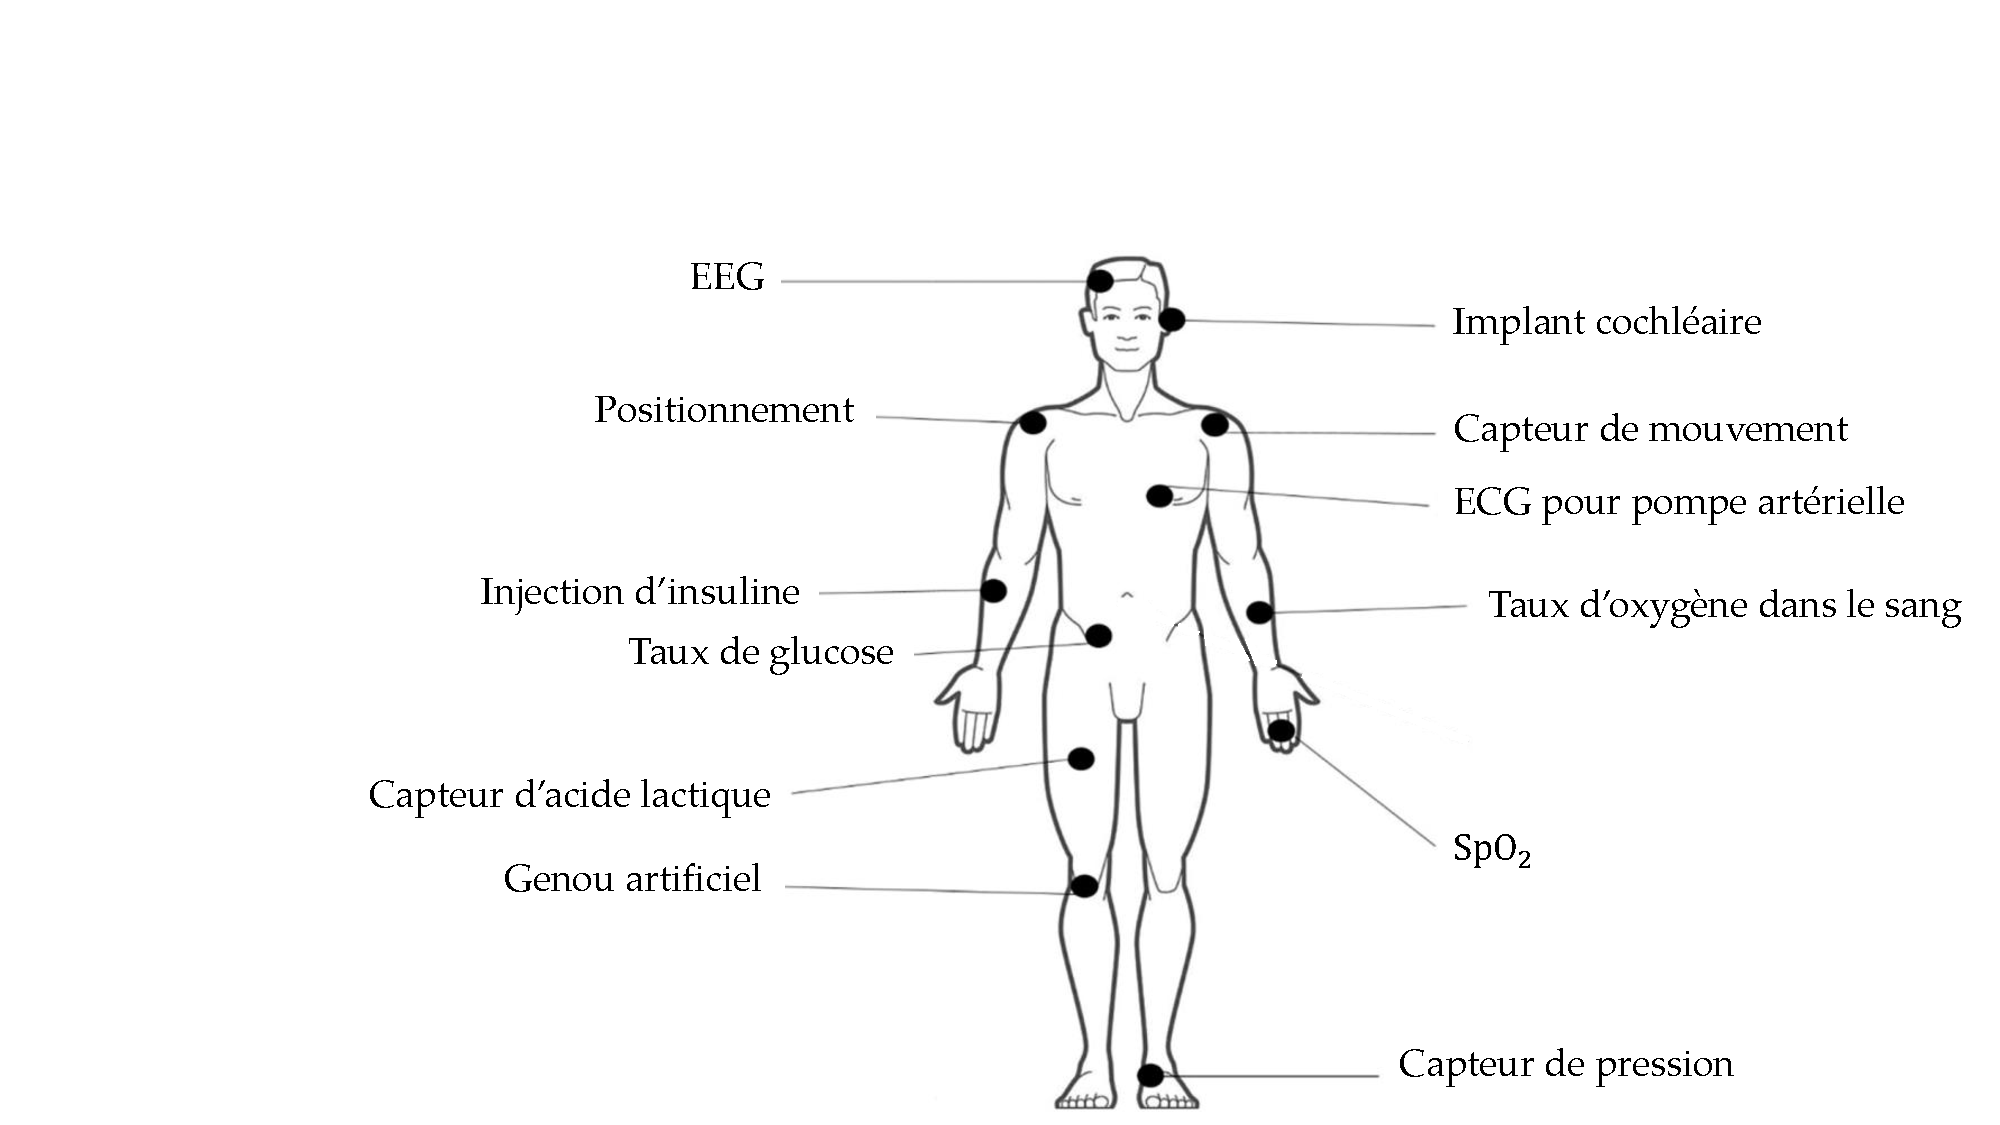
\includegraphics[trim={6cm 0cm 0cm 4cm},clip, width=0.8\textwidth]{../Chap1/Figure/capteurs_corps_humain.pdf}
	\caption{Exemple de WBAN pour la télémédecine \cite{Abidi2020}.}
	\label{fig:capteurs_corps_humain}
\end{figure}
%%%%%%%%%%%%%%%%%%%%%%%%%%%%%%%%%%%%%%%

Enfin, une troisième catégorie d'applications des appareils nomades bio-intégrables est le confort et l'assistance à la personne. Les travaux de Oriowo \emph{et al.} s'inscrivent dans cette catégorie par le développement de lentilles de contact permettant à son porteur de corriger les déficits de reconnaissance des couleurs \cite{Oriowo2011}. Des travaux ont été réalisés par ailleurs sur le développement de gants intelligents, implémentant un réseau de gyroscopes et une intelligence artificielle pour la reconnaissance du langage des signes en arabe \cite{Qaroush2021}. D'autres études encore ont appuyé les avancées sur les développements de prothèses de hanches instrumentées pour l'étude de la charge en compression subie par ces-dernières en fonction des chaussures portées par le patient \cite{Palmowski2021}. Il existe aussi des dispositifs moins invasifs comme les appareils d'aide à l'audition \cite{Qiao2011}. Enfin, le confort et la performance sportive ont motivé la mise en \oe{}uvre et la constante amélioration des accessoires tels que les montres, les bracelets ou les bagues connectés, avec des applications très variées comme la surveillance des constantes vitales, la reconnaissance génétique, ou bien encore les paiements bancaires \cite{Cornelius2014,Kurz2021,VISA2022,FITBIT2022}.

Le tableau \ref{tab:biocapteurs} donne quelques exemples de biocapteurs, ainsi que leurs fonctions et la gamme de puissance. On considère que les puissances élevées sont au-dessus de la dizaine de milliwatts et les puissances très faibles en dessous de la centaine de microwatts. Ces dispositifs peuvent fonctionner simultanément et constituent alors un WBAN sur le corps humain. On présente sur la figure \ref{fig:capteurs_corps_humain} un exemple de configuration de WBAN constitué de divers capteurs et appareils, invasifs et non invasifs, sur l'intégralité du corps humain. Le réseau de transfert de données doit être étudié afin de supprimer toute interférence entre les différents n\oe{}uds communicants.

Le contexte applicatif du corps humain induit alors de la complexité sur plusieurs aspects dans le processus de développement des dispositifs. Certains défis rencontrés sont généralisables et d'autres sont spécifiques à chaque application et sont, en premier lieu, dépendant du caractère invasif du dispositif. Nous allons donc passer en revue la littérature pour identifier ces difficultés avec les réponses qui y ont été apportées et mettre en évidence les défis futurs.
%%%%%%%%%%%%%%%%%%%%%%%%%%%%%%%%%%%%%%
\begin{table}[!htbp]
	\centering
	\resizebox{\textwidth}{!}{%
	\begin{tabular}{l l m{2.1cm} }
\toprule
\rowcolor{blue!10}
\textbf{Capteur}		&	\textbf{Fonction}	& 		\textbf{Consommation de puissance} \\
\midrule
\rowcolor{black!8} 
Température				&Mesurer la température														& Élevée \\ 
Taux de glucose			&Surveiller en continu du taux de glucose dans le sang						& Très faible \\ 
\rowcolor{black!8} 
Électrocardiographe		&(ECG) Mesure le potentiel électrique généré par le c\oe{}ur				& Faible \\
Électromyogramme		&(EMG) Surveiller l'activité musculaire										& Faible \\ 
\rowcolor{black!8} 
Pression sanguine		&Mesurer une pression minimale diastolique et maximale systolique			& Élevée \\ 
Accéléromètre			&Mesurer l'accélération sur tous les axes dans un espace tridimensionnel	& Élevée \\ 
\rowcolor{black!8} 
Visuel					&Traite et fusionne les images d'une scène à partir d'une variété de points de vue		& Élevée \\ 
Gaz CO$_2$				&Surveille les changements des taux de CO$_2$ dans la respiration d'organismes vivants	& Faible \\ 
\rowcolor{black!8} 
Gyroscope				&Mesure l'orientation à l'aide du moment cinétique							& Élevée \\ 
Électroencéphalographie	&(EEG) Surveille l'activité électrique dans le cerveau						& Élevée \\ 
\rowcolor{black!8} 
SpO$_2$					&Mesure la saturation en oxygène pulsé dans le sang						 	& Faible \\
Implant cochléaire		&Aide à l'audition en transposant le son ambiant en signaux électriques		& Faible \\
\bottomrule
		\end{tabular}}
        \caption{Liste non exhaustive de biocapteurs avec leurs fonctions et besoins énergétiques \cite{Abidi2020}}
        \label{tab:biocapteurs}
\end{table}
%/!\/!\/!\/!\/!\/!\/!\/!\/!\/!\/!\/!\/!\/!\/!\/!\/!\/!\/!\/!\/!\/!\/!\/!\%
\section{Mécanique et matériaux pour les applications bio-intégrées}
\label{sec:1.2_Mecanique et materiaux pour les applications bio-integrees}
%/!\/!\/!\/!\/!\/!\/!\/!\/!\/!\/!\/!\/!\/!\/!\/!\/!\/!\/!\/!\/!\/!\/!\/!\%
L'intégration directe des capteurs aux surfaces souples du corps humain impose l'utilisation de matériaux souples, mécaniquement résistants, conducteurs et biocompatibles. Les matériaux les plus développés sont inorganiques. En revanche, leur comportement mécanique fragile et leur module d'élasticité élevé sont intrinsèquement mal adaptés à la bio-intégration \cite{Rogers2010}. De vastes efforts de recherche visent à palier ces problèmes, sans pour autant sacrifier les performances des dispositifs. La flexibilité est un critère primordial. Elle peut être obtenue dans n'importe quel matériau, simplement par des réductions d'épaisseur \cite{Kim2010}. De plus, les textures complexes de la peau et ses mouvements naturels doivent être pris en compte par la grande déformation des matériaux souples. Cette dernière caractéristique mécanique nécessite des matériaux et des conceptions avancés, au-delà de ceux qui reposent simplement sur la réduction de l'épaisseur.

Les stratégies les plus efficaces pour obtenir des matériaux fonctionnels étirables reposent sur des matériaux/composites synthétiques spécialisés ou sur des assemblages hétérogènes de micro/nanostructures de matériaux. La première fait appel à des matériaux intrinsèquement étirables basés sur le dopage au moyen de produits chimiques organiques ou inorganiques spécialement formulés. La seconde, exploite des composites qui combinent des fils, des membranes, des rubans ou des plaquettes ultra-minces, typiquement à l'échelle nanométrique, de matériaux établis de haute performance (par exemple, le silicium, les métaux) avec des substrats mous pour produire des systèmes avec une extensibilité efficace \cite{Ray2019}. Des articles de synthèse récents donnent des informations complémentaires et plus détaillés à ce sujet \cite{Lee2017,Lou2018}. 

La littérature propose trois stratégies principales pour l'optimisation des performances et de l'intégrabilité des applications nomades sur le corps humain : matériau ; topologie et structure ;système. Les sous-sections qui suivent présentent un résumé des avancées et défis majeurs rencontrés en fonction de la stratégie adoptée.
    %/////////////////////////////////////////////
	\subsection{Stratégie d'optimisation matériau}
	\label{subsec:1.2.1_Strategie materiau}
	%////////////////////////////////////////////
Dans la catégorie de la synthèse de matériaux adaptée aux applications bio-compatibles et bio-intégrables on retrouve trois classifications que sont :
\begin{itemize}[label=$\bullet$]
	\item Les polymères intrinsèquement extensibles.
 	\item Les hydrogels et gels ioniques.
 	\item Les mélanges hétérogènes de matériaux élastiques isolants et de matériaux conducteurs, ou bien l'assemblage laminaire de ces derniers, ou bien encore de structures élastomères diélectriques (\emph{DE}).
\end{itemize}

Comparé aux matériaux inorganiques à module d'élasticité élevé, les matériaux organiques tels que les polymères conducteurs et semi-conducteurs combinent la souplesse et la biocompatibilité, avec des caractéristiques optiques, mécaniques et électriques intéressantes. La conductivité et la souplesse de ces matériaux peuvent être augmentées par le biais d'additifs ioniques, mais ces derniers augmentent la toxicité du matériau, ce qui limite leur emploi pour des applications bio-intégrées. Aussi, la copolymérisation \cite{Muller2007} et l'introduction d'éléments chimiques dans les mailles cristallines \cite{Wang2016b} constituent deux méthodes supplémentaires pour l'amélioration de leur souplesse.

Les hydrogels et les gels ioniques constituent une deuxième catégorie de matériaux actifs étirables, remarquables par leur étroite imitation des propriétés mécaniques, chimiques et optiques des tissus biologiques. Les principaux défis posés par les hydrogels consistent à obtenir une forte adhésion à d'autres matériaux et à éviter les changements progressifs de propriétés dus à l'évaporation de l'eau. Des travaux récents ont été réalisés pour l'amélioration de l'adhésion chimique \cite{Tang2016}. Des approches avancées remplacent par ailleurs l'eau par des liquides ioniques à température ambiante, plus stables par rapport au séchage par évaporation \cite{Xie2018}.

Les composites représentent la troisième catégorie de la stratégie d'optimisation matériau \cite{Li2007}. Le défi principal est la proportionnalité inverse entre la conductivité et la souplesse des composites. Les \emph{DE} sont un cas particulier de l'assemblage de ces éléments. Ce sont des transducteurs composés d'une membrane de polymère en sandwich entre deux électrodes. Les études récentes sur l'optimisation des \emph{DE} montrent des améliorations notables sur leurs performances électro-mécaniques \cite{Lu2020}. Cependant, les limites de leur utilisation se trouvent dans les fortes tensions d'actionnement, les faibles résistances au claquage électrique, le fort hystérésis, mais aussi la faible fiabilité \cite{Zhao2010,Lv2018}.
    %////////////////////////////////////////////
	\subsection{Stratégie d'optimisation topologique et structurelle}
	\label{subsec:1.2.2_Strategie numerique}
	%////////////////////////////////////////////
Lorsque les limites de l'optimisation physico-chimique des matériaux sont atteintes, la solution peut être de se tourner vers des conceptions adaptées aux applications afin d'améliorer l'intégrabilité et les performances des dispositifs bio-intégrables. Deux outils majeurs sont considérés dans la littérature afin de répondre à la problématique : l'optimisation topologique et l'optimisation structurelle.

L'optimisation topologique des dispositifs bio-intégrables consiste à adapter leur interface de liaison avec les tissus mous du corps humain afin de faciliter leur intégrabilité, augmenter leurs performances ou bien améliorer le confort de l'utilisateur. L'optimisation structurelle, quant à elle, consiste à adapter la structure générale du dispositif avec les mêmes objectifs. Ces procédés se divisent généralement en trois phases. La première phase passe par la numérisation tri-dimensionnelle(3D) de la surface d'intérêt sur le corps humain et la seconde consiste à modifier de façon numérique la surface du dispositif pour l'adapter. Enfin, la troisième phase se concentre sur la fabrication au moyen de la technologie de fabrication additive comme le moulage, l'impression 3D ou bien les dépôts de couches minces \cite{Mennad2015}. Les principales techniques de numérisation 3D ont été résumées dans les travaux de thèse de Coudert \cite{Coudert2005}. L'optimisation topologique consiste ensuite à générer des algorithmes de calcul capables de transformer un jeu de paramètres multiphysiques et un jeu de contraintes associé, en une géométrie topologique ou structurelle favorisant les performances et l'intégrabilité du dispositif \cite{Liu2018}.

Les principaux défis de la phase de numérisation et optimisation algorithmique 3D reposent sur la fiabilité de la reconstitution. Les algorithmes d'optimisation trouvent par ailleurs leurs limites dans la faisabilité de la géométrie résultante qui nécessite généralement une correction sur la densité structurelle \cite{Zegard2016} ou bien sa définition implicite \cite{Vogiatzis2017} afin de rendre possible sa fabrication. 
    %////////////////////////////////////////////
	\subsection{Stratégie d'optimisation système}
	\label{subsec:1.2.3_Strategie systeme}
	%////////////////////////////////////////////
L'optimisation matériau est un processus qui requière généralement une très grande durée de développement, car la synthèse de matériaux est un domaine qui met en évidence des phénomènes encore non expliqués par la communauté de chercheurs concernés. En outre, l'optimisation numérique de la topologie ou des structures trouve ses limites entre la faisabilité et les performances offertes par la géométrie résultante. Une approche alternative pour l'optimisation des dispositifs visant la bio-intégration est d'adopter une vision système. En ce sens, la solution peut être de s'appuyer sur une combinaison innovante de sous-systèmes dont le fonctionnement et les performances intéressantes ont déjà pu être démontrés dans la littérature. Cette démarche apporte un nouveau champ de réalisations possibles pour des applications dont la fonction primaire devient une fonction secondaire dans un ensemble plus large répondant à un besoin spécifique. De nombreuses études entrent dans cette stratégie d'approche, sans pour autant la mettre en évidence. Voici trois exemples d'applications permettant d'illustrer cette méthode de développement.
\begin{figure}[!htbp] 
\centering
\captionsetup{justification=centering}
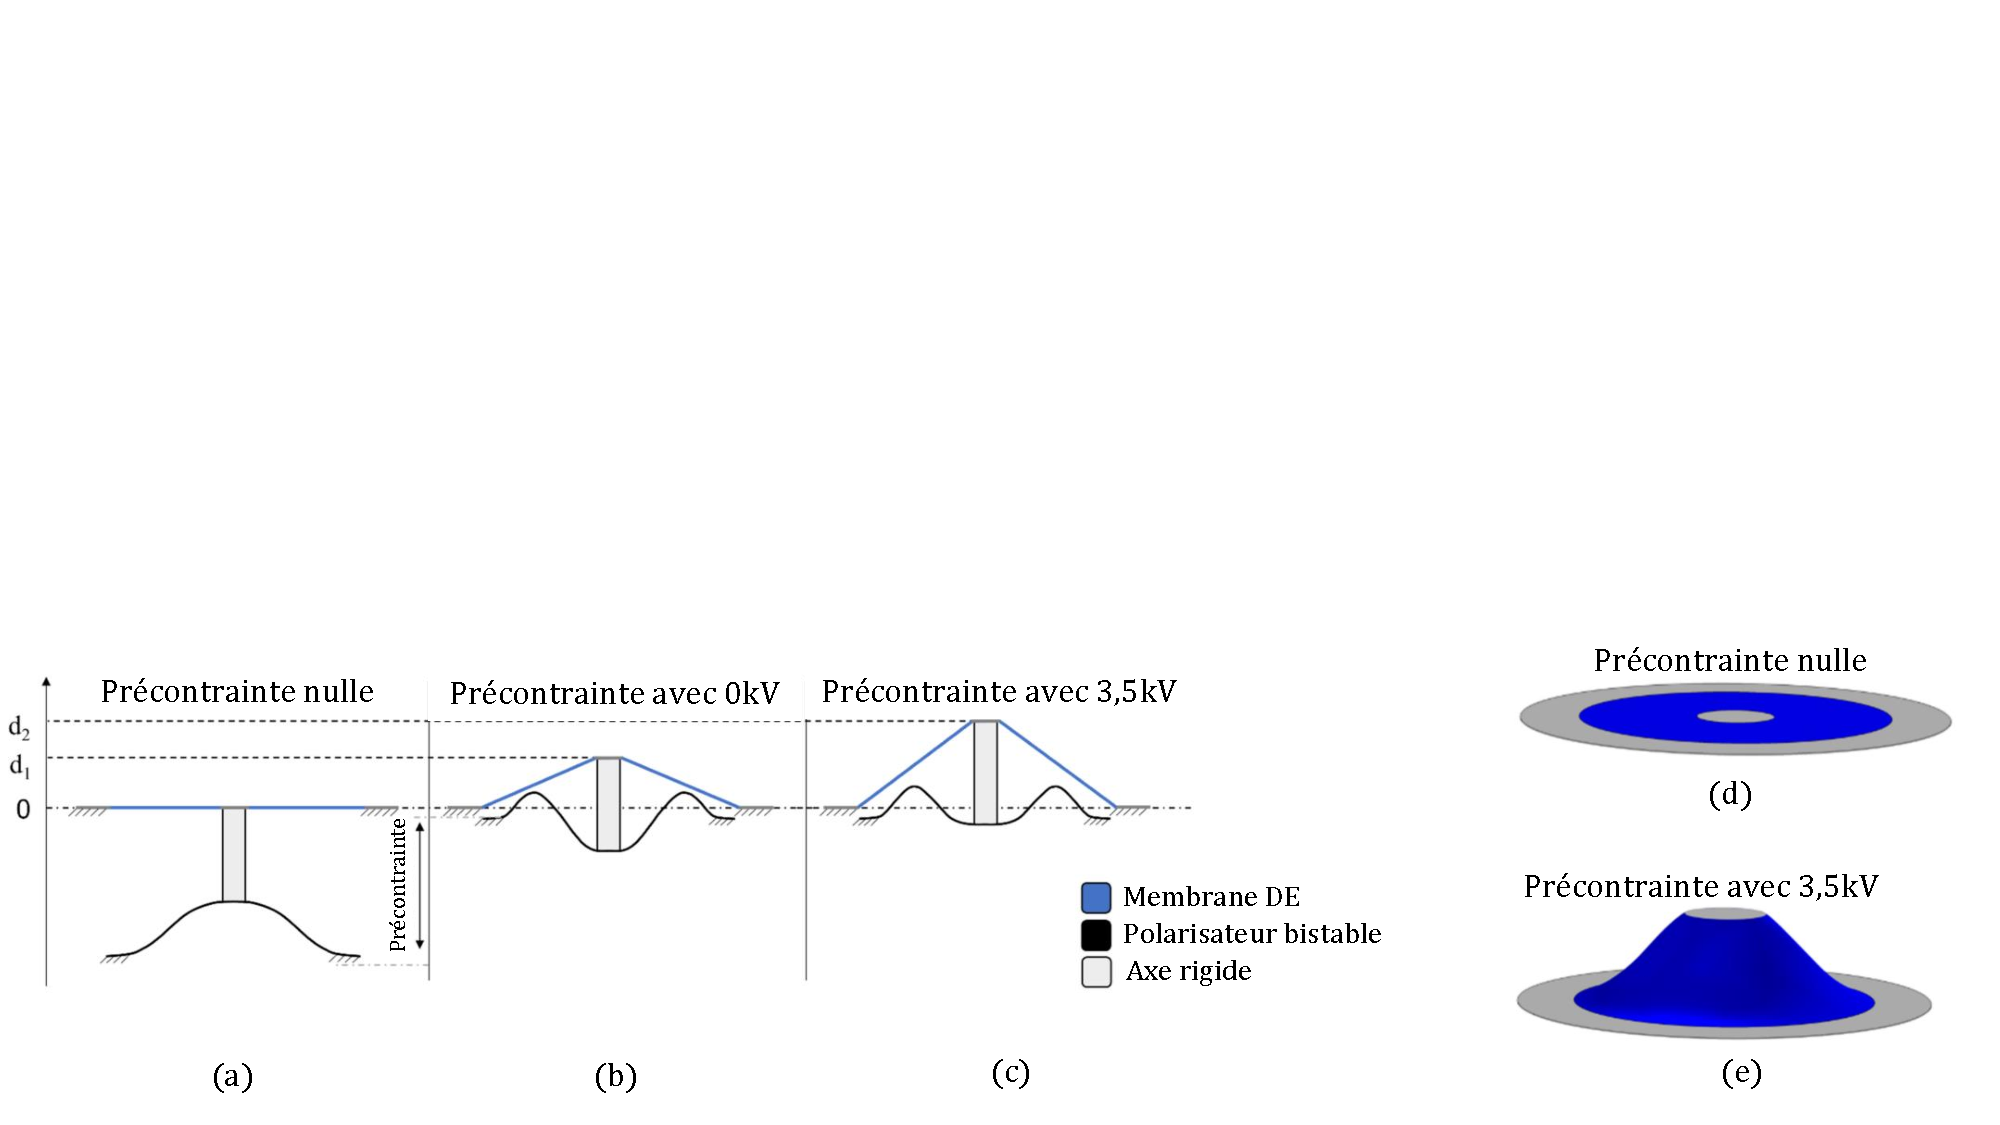
\includegraphics[trim={0cm 0cm 0cm 10cm},clip, width=\textwidth]{../Chap1/Figure/DEA.pdf}
\caption{Prorotype d'actionneur \emph{DE} mécaniquement optimisé \cite{Croce2021}.\\
		 (a,b,c) Schématisation de trois positions stables en fonction de la précontrainte et de la tension entre les électrodes. (d,e) Vue 3D du prototype avec la membrane \emph{DE} non déformée et déformée}
\label{fig:DEA}
\end{figure}

Croce \emph{et al.} ont récemment travaillé sur l'optimisation des performances d'actionneurs à base de \emph{DE} \cite{Croce2021}. La simple implémentation d'un ressort non linéaire, composé de lames d'acier dans une architecture bistable, a permis d'obtenir des courses d'actionneur plus intéressantes que les solutions classiques à ressort linéaire. La figure \ref{fig:DEA} montre une vue schématisée des trois positions stables de l'actionneur. 
% Plus en lien avec la récupération d'énergie, Izadgoshasb \emph{et al.} ont travaillé sur l'optimisation d'un récupérateur piézoélectrique pour l'exploitation de l'énergie cinétique de marche \cite{Izadgoshasb2018}. La figure \ref{fig:PEH_tibia_photo} montre un aperçu du prototype. Ce dernier est composé d'une poutre en porte à faux implémentant une masse dynamique à l'extrémité libre et un patch piézoélectrique à l'extrémité encastrée. Ce travail a notamment permis d'estimer l'orientation optimale de la poutre (\ang{70}) pour maximiser la puissance de sortie du générateur (fig. \ref{fig:PEH_tibia_schema}). L'intégration sur le corps humain est réalisé grâce à un simple bandage avec une partie rigide où vient se fixer la poutre. Il ne serait pas possible d'exploiter la résonance de telles structures oscillantes avec un interfaçage cutané. En effet, l'idée principale exploitée ici est d'utiliser le bandage comme interface de transfert d'énergie pour déporter celle-ci. Ainsi, il devient possible d'intégrer des structures oscillantes telle que celle présentée ici. Les performances pourraient néanmoins être améliorées au moyen d'optimisations électromécaniques diverses pour une récupération large bande. Ces dernières seront explicitées en section \ref{subsec:1.3.4_Solutions technologiques pour l amelioration des recuperateurs}.
% %%%%%%%%%%%%%%%%%%%%%%%%%%%%%%
% \begin{figure}[!htbp]
% 	\begin{center}
% 		\begin{subfigure}[t]{0.4\textwidth}
% 			\captionsetup{justification=centering}
% 			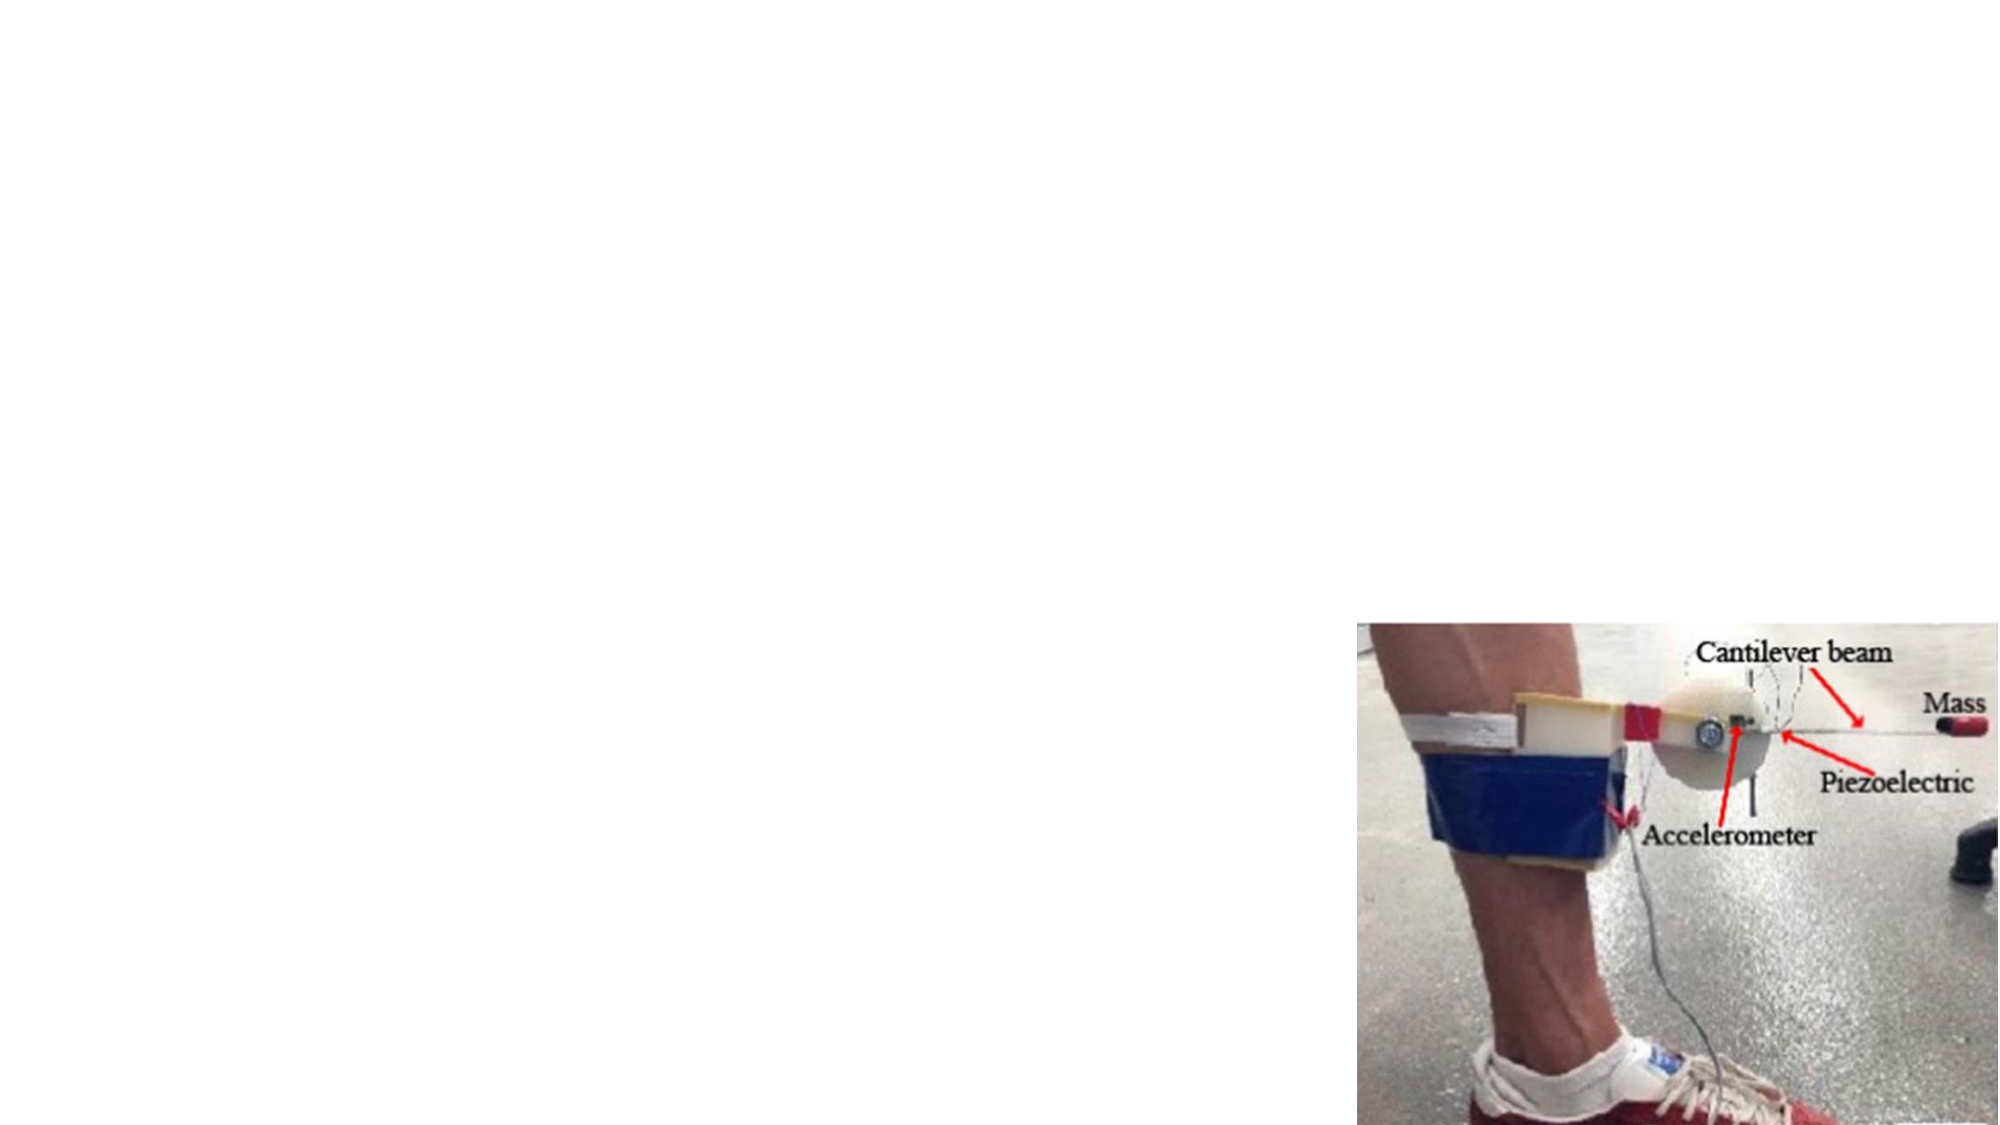
\includegraphics[trim={23cm 0cm 0cm 10.5cm},clip,width=\textwidth]{../Chap1/Figure/PEH_tibia_photo.pdf}
% 			\caption{Illustration du prototype accroché sur un tibia}
% 			\label{fig:PEH_tibia_photo}
% 		\end{subfigure}
% 		\hfillx
% 		\begin{subfigure}[t]{0.3\textwidth}
% 			\captionsetup{justification=centering}
% 			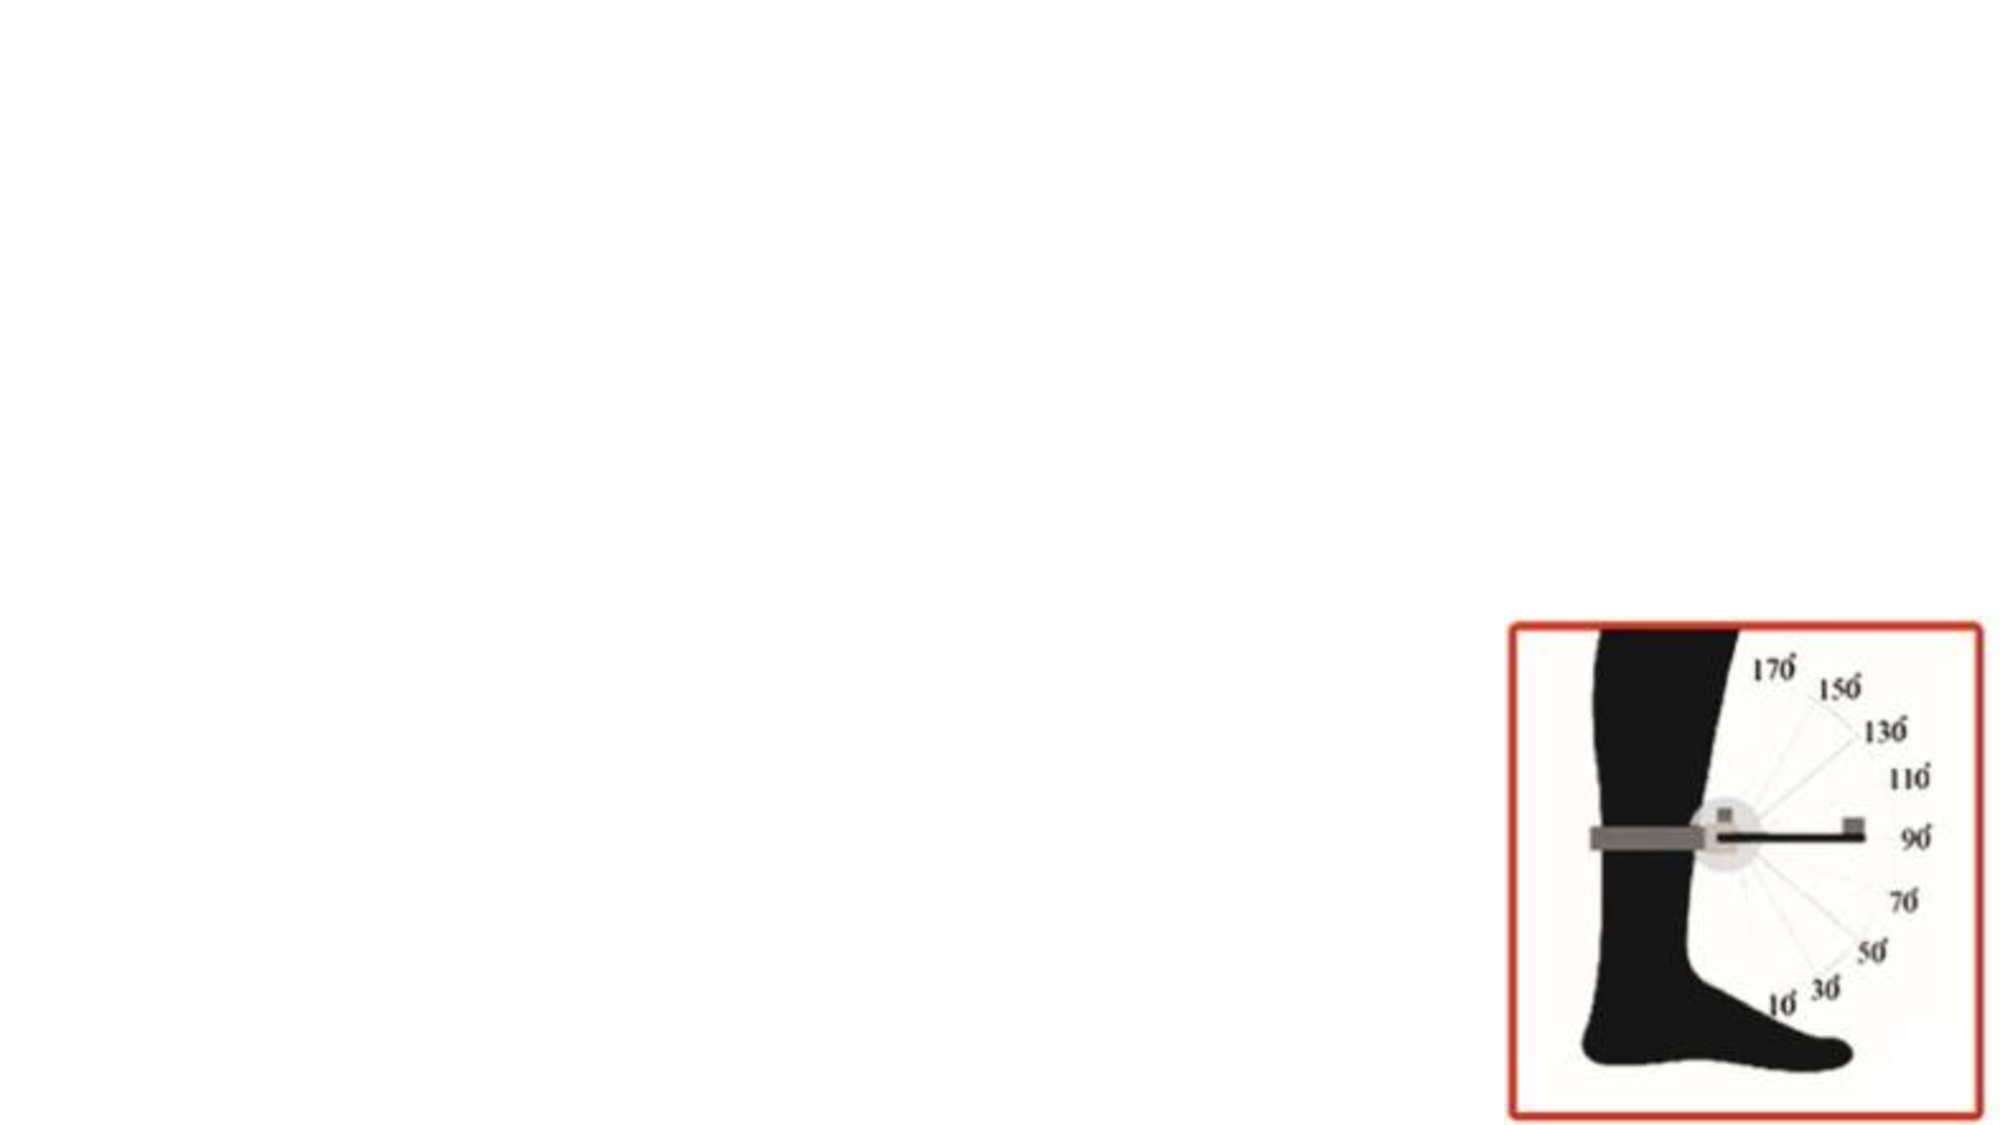
\includegraphics[trim={25.3cm 0cm 0cm 10.5cm},clip,width=\textwidth]{../Chap1/Figure/PEH_tibia_schema.pdf}
% 			\caption{Orientation du générateur piézoélectrique}
% 			\label{fig:PEH_tibia_schema}
% 		\end{subfigure}
% 		\caption{Dispositif de récupération de l'énergie cinétique de marche \cite{Izadgoshasb2018}}
% 		\label{fig:PEH_tibia}
% 	\end{center}
% \end{figure}
% %%%%%%%%%%%%%%%%%%%%%%%%%%%%%%

Un autre exemple, en rapport direct avec ce sujet de thèse, est illustré sur la figure \ref{fig:earplug}. Les chercheurs de l'École de Technologie Supérieure de Montréal ont  mené des travaux visant à améliorer le contact entre la paroi du conduit auditif (CA) et celle d'un bouchon intra-auriculaire \cite{Voix2002}. Ces travaux visent à améliorer la qualité du son, le confort et le maintien en position d'écouteurs intra-auriculaires dans des environnements très bruyants comme celui des porte-avions ou des chantiers de construction. La figure \ref{fig:earplug} montre un aperçu du concept ainsi développé pour répondre à la problématique. Ce dernier consiste à mouler un dispositif adapté à chaque individu de façon intra-auriculaire. Le procédé consiste à injecter du silicone liquide sous pression entre un élément rigide et une enveloppe souple extensible. Deux microphones sont alors placés, respectivement à l'extérieur et à l'intérieur du CA, afin de caractériser la réduction de bruit. La bio-intégrabilité du dispositif a été perfectionnée dans ces travaux pas le moyen de procédé de moulage avec l'utilisation de matériaux souples classiques. La géométrie variable des tissus mous de la paroi du CA pourrait nécessiter une optimisation numérique de la topologie d'un dispositif visant à maximiser la surface de contact avec la peau. La grande conformité géométrique est obtenue dans ce cas précis par thermoformage direct sur le sujet humain. C'est à la suite de ces travaux que la source d'énergie, exploitée dans ces travaux de thèse, a pu être mise en évidence et partiellement caractérisée.
%%%%%%%%%%%%%%%%%%%%%%%%%%%%%%
\begin{figure}[!htbp]
	\centering
	\captionsetup{justification=centering}
	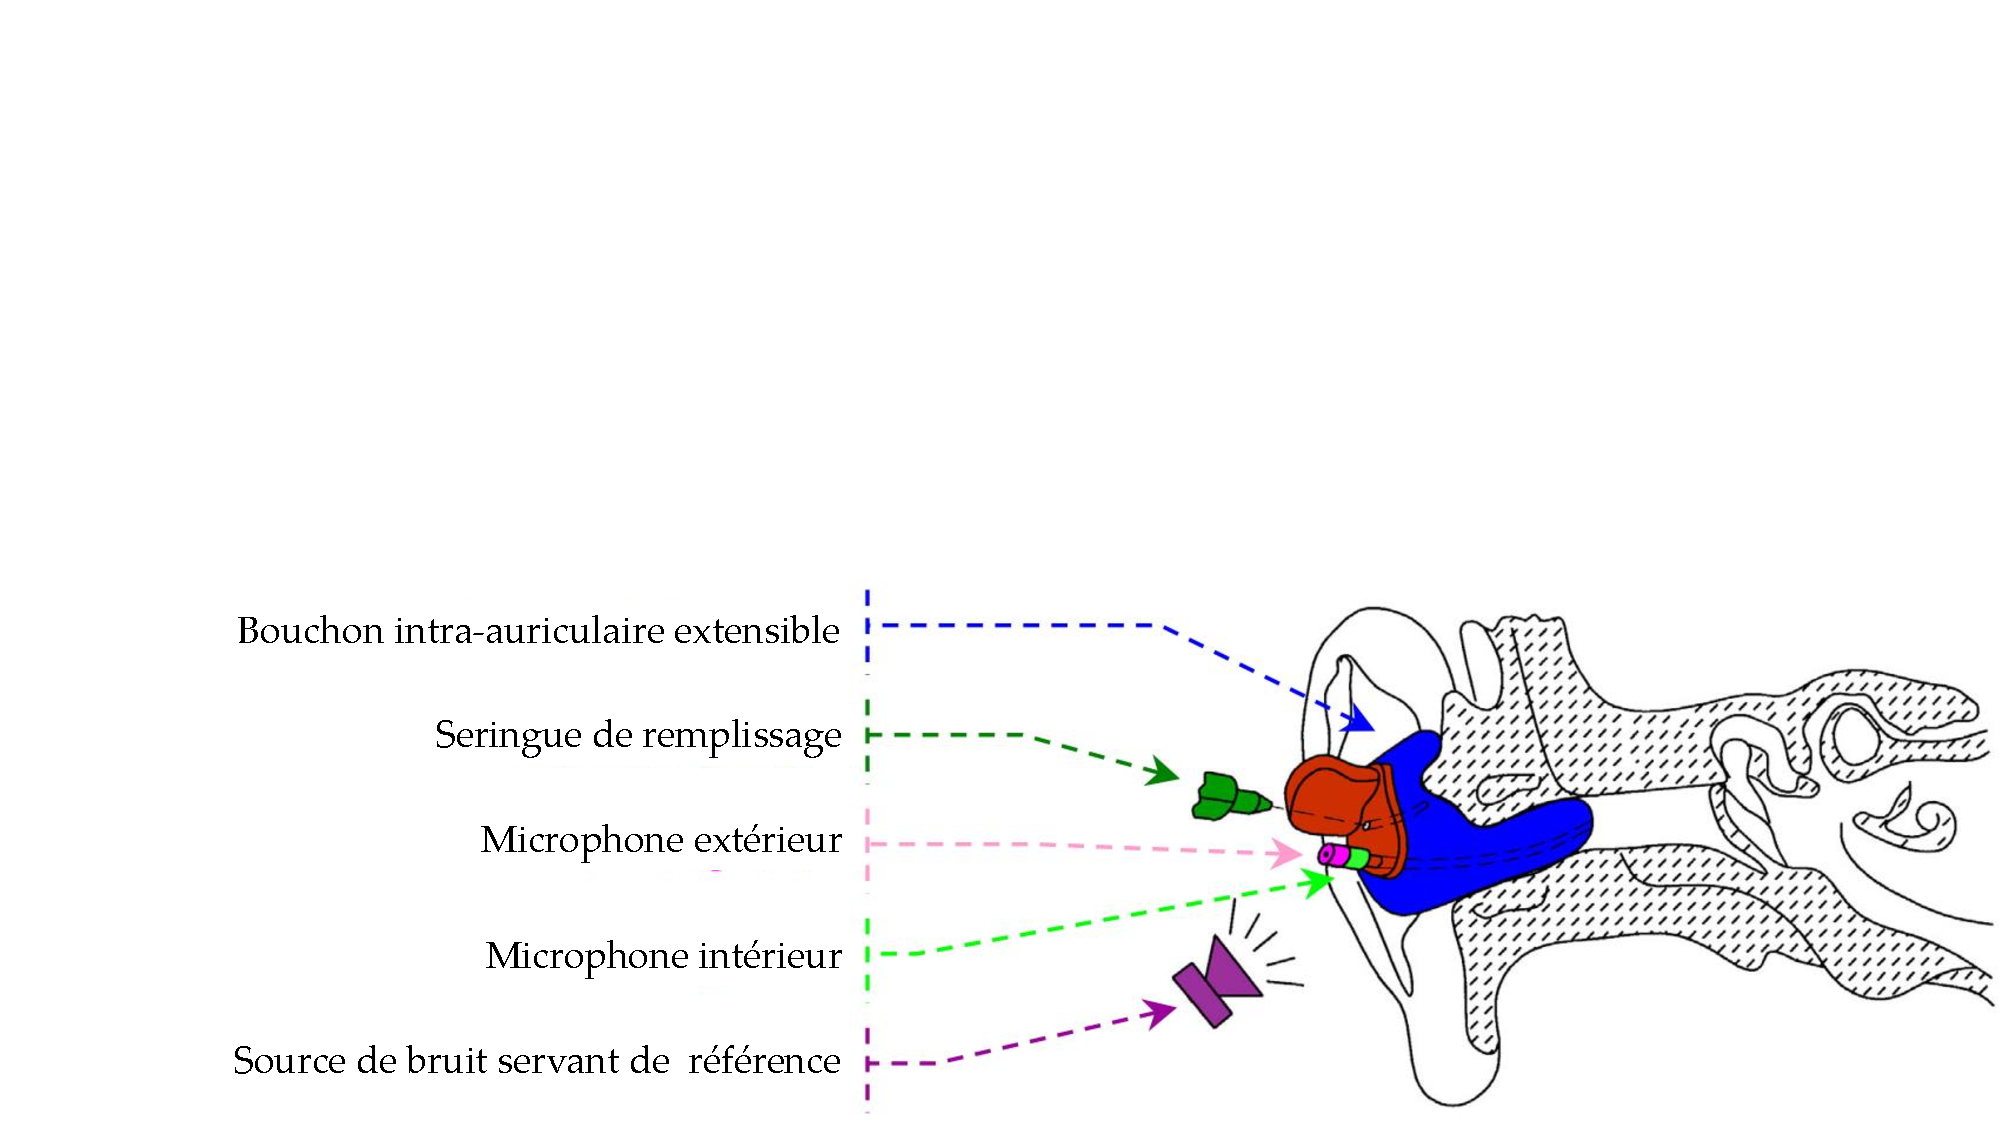
\includegraphics[trim={3.8cm 0cm 0cm 10cm},clip, width=\textwidth]{../Chap1/Figure/earplug.pdf}
	\caption{Concept de bouchon d'oreille proposé par Voix et Laville \cite{Voix2002}}
	\label{fig:earplug}
\end{figure}
%%%%%%%%%%%%%%%%%%%%%%%%%%%%%%
% fait partie des moyens d'alimentation alternatifs en électricité pour les  la transition dans travaux de cette thèse sur le même principe, et plus en lien avec le sujet de la thèse, on retrouve les travaux de Smilek fait partie des moyens d'alimentation alternatifs en électricité pour les  la transition dans travaux de cette thèse sur le même principe, et plus en lien avec le sujet de la thèse,

Ce dernier exemple entre dans le cadre de la récupération d'énergie et pourra servir d'introduction à la section qui suit. Smilek \emph{et al.} ont travaillé sur un récupérateur électromagnétique visant l'exploitation de l'énergie cinétique de la marche \cite{Smilek2016}. Le dispositif est présenté sur la figure \ref{fig:kinetic_energy_head_head}. Le système est conçu pour s'intégrer au niveau de la tête afin d'alimenter des appareils nomades de type implant cochléaire. Il serait difficile d'exploiter la résonance de telles structures avec un interfaçage cutané à cause de la souplesse de la peau qui absorbe naturellement l'énergie cinétique de marche. En effet, l'idée principale exploitée ici est d'utiliser le bandage comme interface de transfert d'énergie pour déporter celle-ci. Ainsi, cela simplifie le développement et l'implémentation de structures oscillantes telle que celle présentée ici. La densité de puissance récupérée sur 5 sujets varie de 30µW/cm$^3$ à 119µW/cm$^3$ en marche normale et de 50µW/cm$^3$ à 239µW/cm$^3$ en marche rapide.
%%%%%%%%%%%%%%%%%%%%%%%%%%%%%%
\begin{figure}[!htbp]
	\centering
	\captionsetup{justification=centering}
	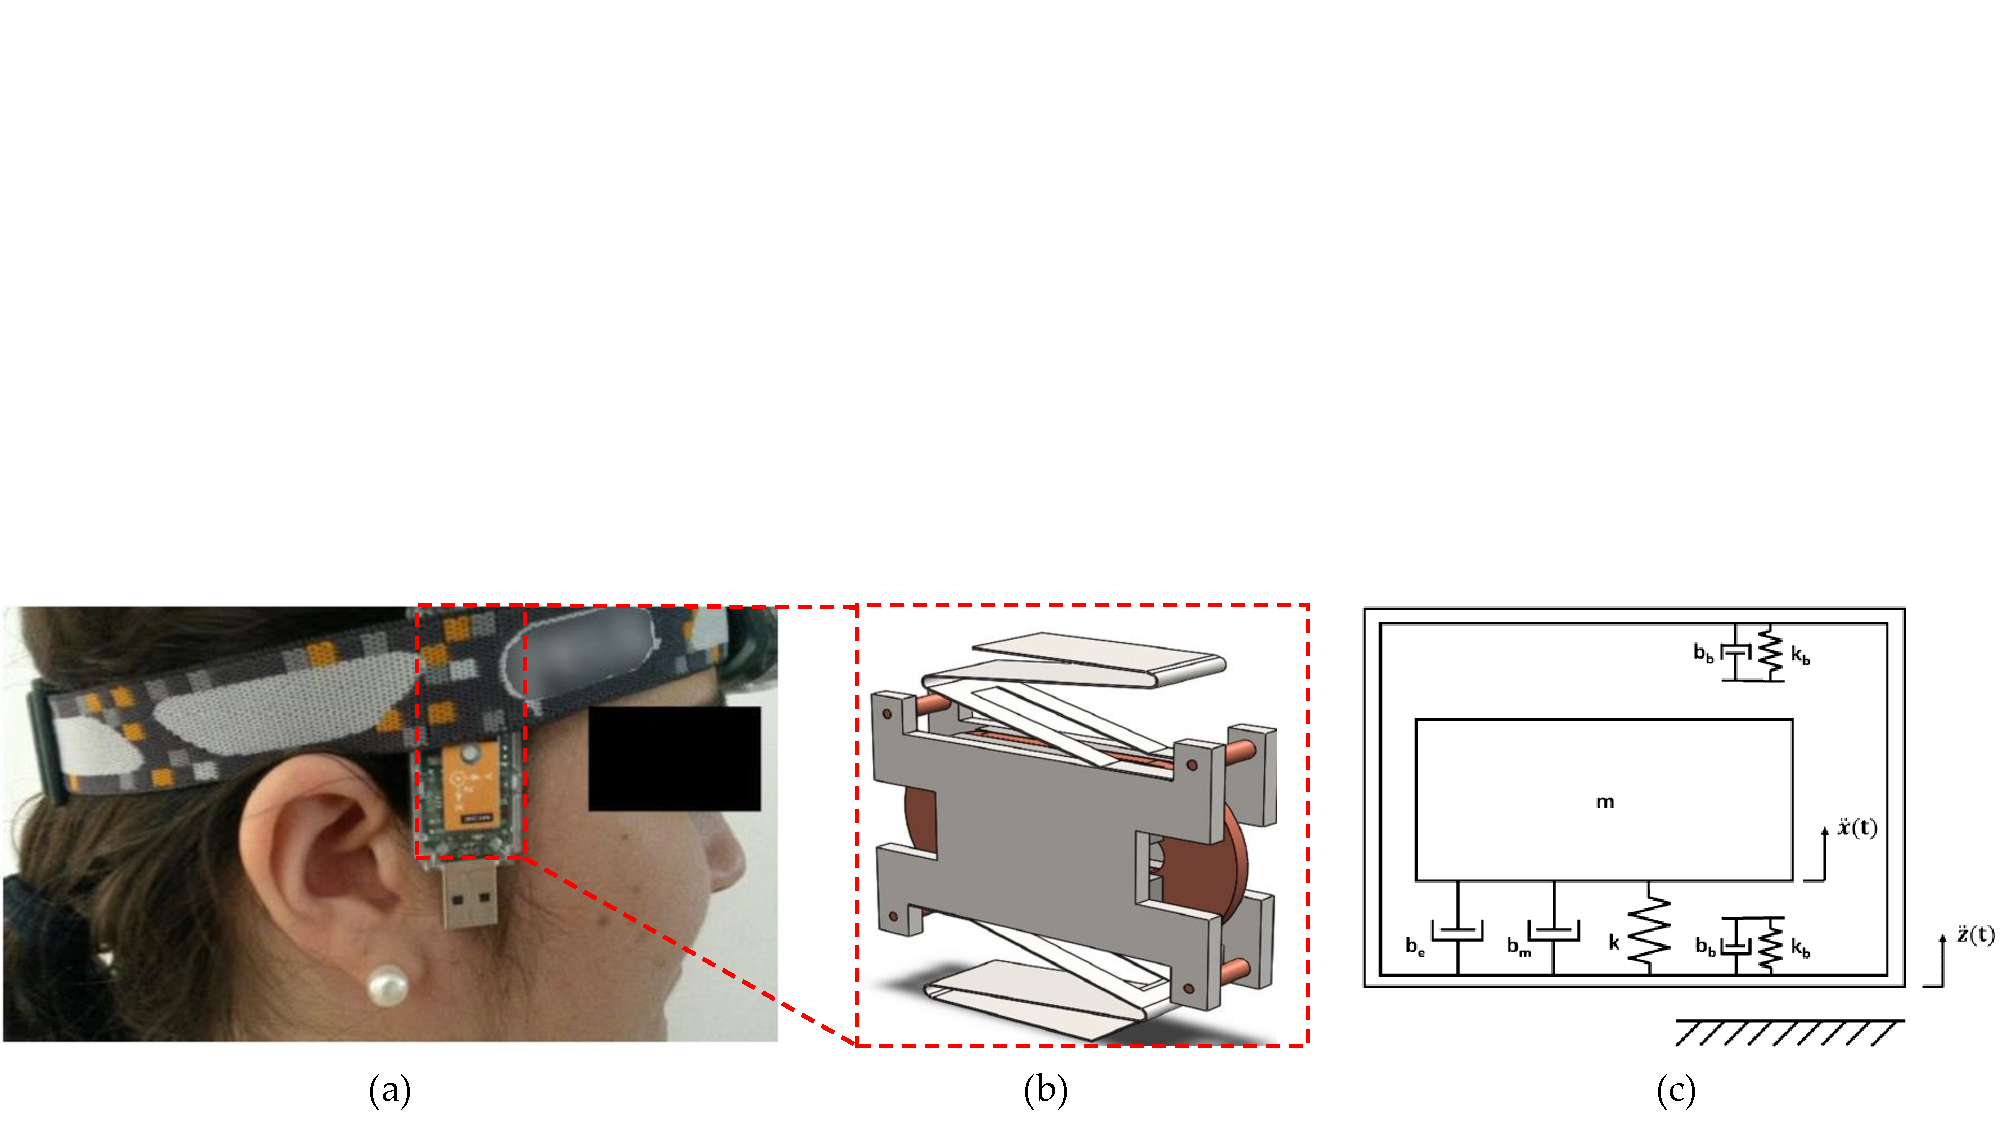
\includegraphics[trim={0cm 0cm 0cm 10cm},clip,width=\textwidth]{../Chap1/Figure/kinetic_energy_head.pdf}
	\caption{(a) : Image du prototype encapsulé installé sur un crâne. (b) : Vue 3D du convertisseur. (c) : Schéma de modélisation du convertisseur \cite{Smilek2016}}
	\label{fig:kinetic_energy_head_head}
\end{figure}
%%%%%%%%%%%%%%%%%%%%%%%%%%%%%%

Ces trois exemples montrent que le développement des nouvelles technologies performantes pour les applications électromécaniques bio-intégrées apparaît possible par l'implémentation ingénieuse de matériaux spécifiques au sein de processus mécaniques simples. L'intérêt majeur réside dans les performances intrinsèques de ces-derniers, qui ont généralement été démontrées à de multiples reprises dans la littérature. Le travail de cette thèse s'inscrit dans cette catégorie d'optimisation, dans une certaine mesure qui sera explicitée dans le chapitre \ref{ch:2_Modelisation et simulation du systeme}.

La section qui suit entre plus en détails sur les aspects énergétiques des appareils nomades.
%/!\/!\/!\/!\/!\/!\/!\/!\/!\/!\/!\/!\/!\/!\/!\/!\/!\/!\/!\/!\/!\/!\/!\/!\%
\section{Gestion de puissance et efficacité énergétique}
\label{sec:1.3_Gestion de puissance et efficacite energetique}
%/!\/!\/!\/!\/!\/!\/!\/!\/!\/!\/!\/!\/!\/!\/!\/!\/!\/!\/!\/!\/!\/!\/!\/!\%
Le besoin énergétique pour le fonctionnement des applications nomades, intégrables sur/dans le corps humain, motive la recherche dans le développement de systèmes à faible consommation d'énergie. De plus, l'émergence de technologies de récupération d'énergie de plus en plus performantes permet d'améliorer l'autonomie des dispositifs, et dans certains cas, de les rendre entièrement autonomes. 
    %////////////////////////////////////////////
	\subsection{Architecture des appareils nomades}
	\label{subsec:1.3.1_Architecture des appareils nomades}
	%////////////////////////////////////////////
L'architecture générale des dispositifs nomades est présentée sur la figure \ref{fig:noeud_capteur-actionneur} et les fonctions respectives de chacun des composants sont décrites dans le tableau \ref{tab:fonctions_compsantes_architecture_IOT}. Ces-derniers ne sont pas tous indispensables au fonctionnement du dispositif, car leur présence est conditionnée par les tâches à réaliser. En ce sens, les invariants dans l'architecture sont : le microprocesseur, le circuit de gestion de puissance et de stockage, ainsi que le(s) unité(s) de stockage d'énergie. Trois configurations classiques comprenant les composants essentiels sont les suivantes :
\begin{itemize}[label=$\circ$]
	\item \emph{Le capteur autonome} : composants essentiels + élément sensible + conditionneur + transmetteur. Ex., bracelet capable de capter de présence de gaz spécifique \cite{Choi2016}.
	\item \emph{L'actionneur autonome} : composants essentiels + transducteur. Ex., un muscle artificiel à base de matériaux électro-élasto-cinématiques microstructurés \cite{Lee2016}. 
	\item \emph{Le dispositif hybride} : Composants du capteur + composants de l'actionneur. Ex, un implant cochléaire capable de capter le son ambiant et de générer des signaux électriques interprétables par le cerveau. \cite{Yip2015}
\end{itemize}
Le caractère autonome des dispositifs fait ici référence à leur fonctionnement général qui est piloté par le programme contenu dans le microcontrôleur. On parle par ailleurs d'autonomie énergétique lorsque le sous-système de récupération d'énergie génère, à lui seul, suffisamment de puissance pour maintenir leur fonctionnement.
%%%%%%%%%%%%%%%%%%%%%%%%%%%%%%%%%%%%%%
\begin{figure}[!htbp]
\centering
\captionsetup{justification=centering}
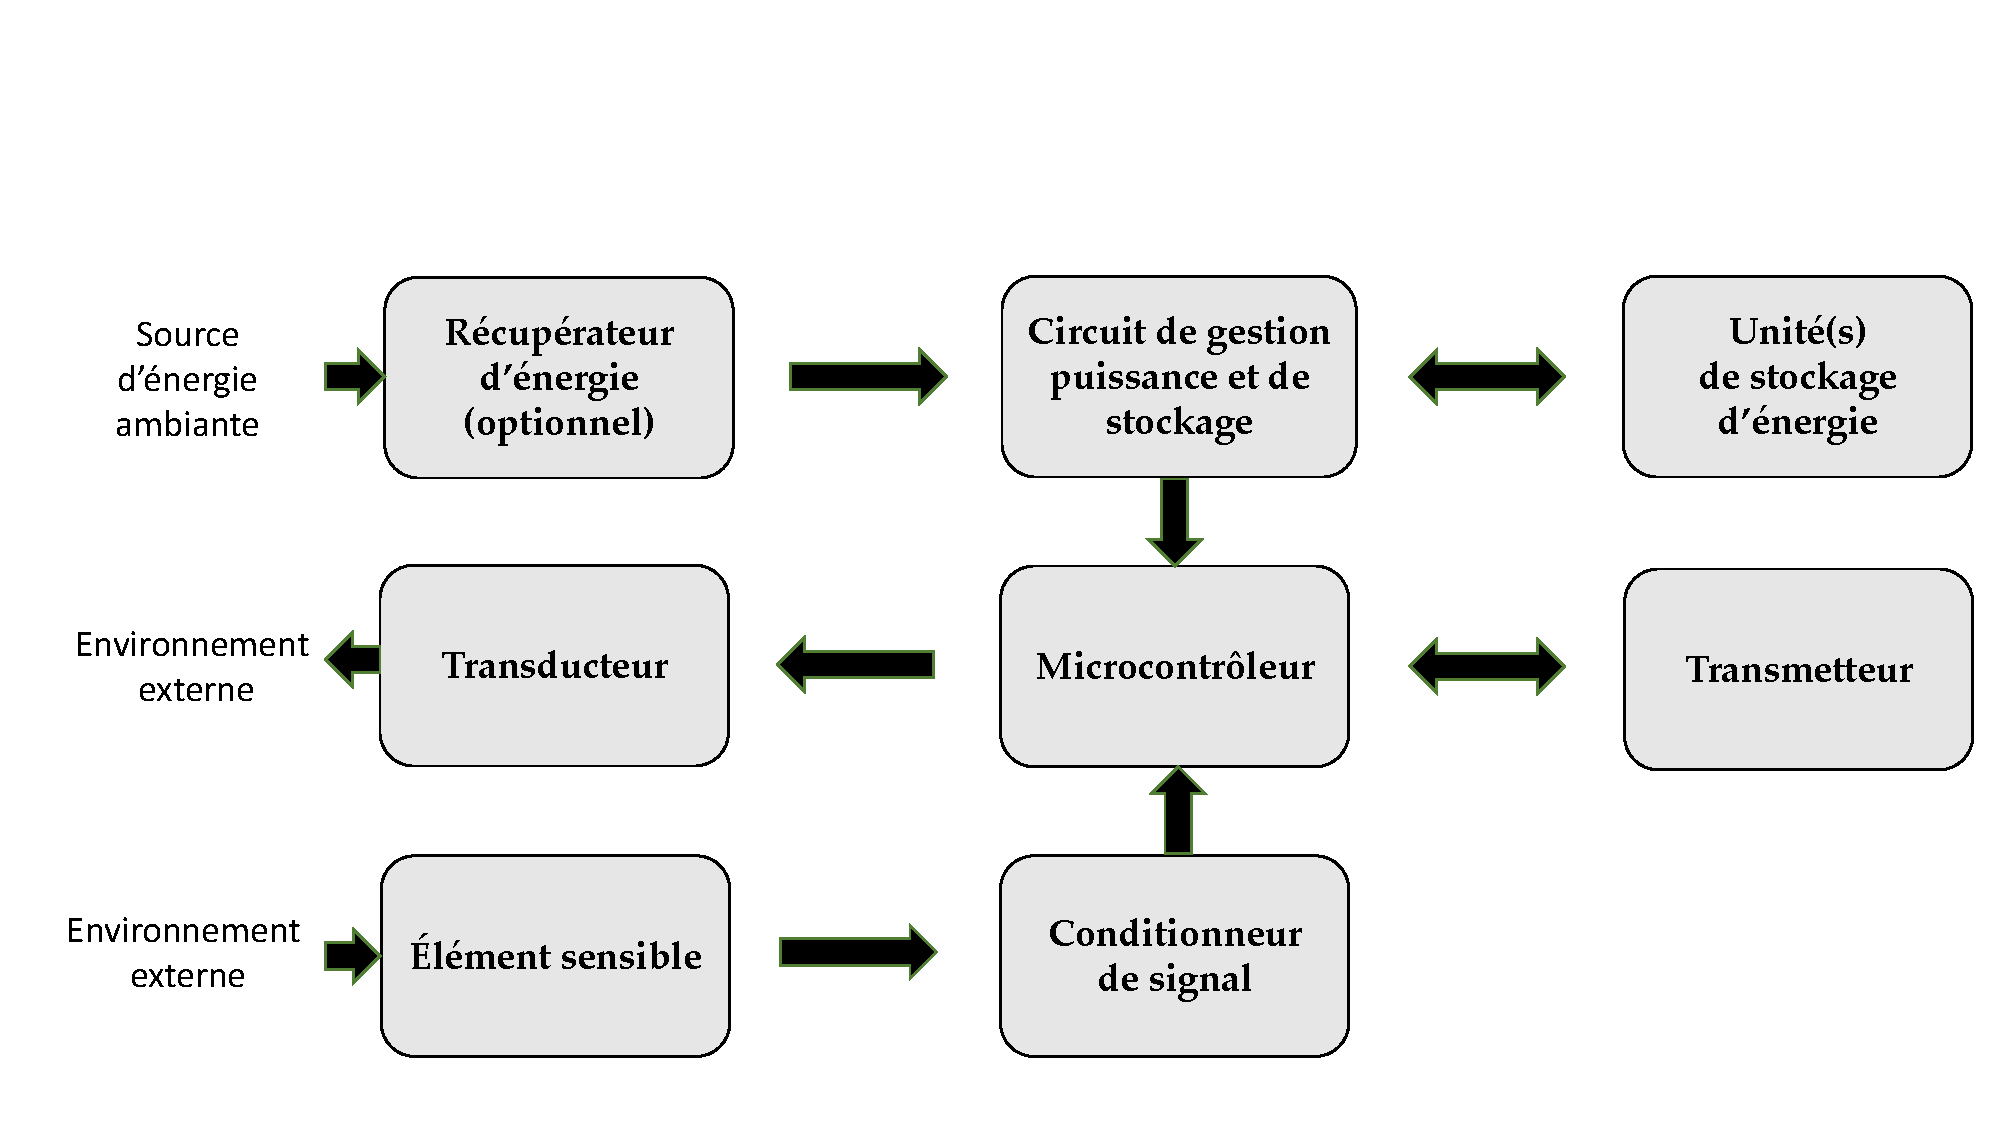
\includegraphics[trim={0.7cm 0cm 0cm 3.5cm},clip, width=0.9\textwidth]{../Chap1/Figure/noeud_capteur-actionneur.pdf}
\caption{Architecture de dispositif nomade \cite{Borole2021}}
\label{fig:noeud_capteur-actionneur}
\end{figure}
%%%%%%%%%%%%%%%%%%%%%%%%%%%%%%%%%%%%%%%
\begin{table}[!htbp]
	\centering
	\resizebox{\textwidth}{!}{%
	\begin{tabular}{m{2.5cm} m{12cm} }
\toprule
\rowcolor{blue!10}
\textbf{Composant}		&	\textbf{Fonction}\\
\midrule
\rowcolor{black!8} 
Microcontrôleur									&
Le microcontrôleur est un circuit intégré programmable incluant généralement un processeur, une mémoire et des entrées/sorties sur une même puce électronique. Il coordonne et traite les informations des composants environnants. \\ 
Circuit de gestion de puissance et de stockage		& 
Le circuit de gestion de puissance et de stockage va permettre, d'une part, de réguler et contrôler la puissance consommée par les différents composants. D'autre part, il va redresser et stabiliser l'énergie transmise par le récupérateur, afin de la stocker dans une batterie rechargeable. \\
\rowcolor{black!8} 
Récupérateur d'énergie 							& 
Le récupérateur d'énergie va exploiter l'énergie disponible dans l'environnement du dispositif afin de la convertir en électricité.\\
Unité(s) de \mbox{stockage}							&
Composés d'une ou plusieurs unités, les supercondensateurs et les batteries remplissent ce rôle par leur capacité à stocker l'énergie. Ils peuvent être rechargeables en fonction de la présence ou non d'un système de récupération d'énergie. \\
\rowcolor{black!8} 
Transducteur										&
Le transducteur génère un signal physique et/ou chimique dans le but d'agir sur l'environnement extérieur en fonction des commandes envoyées par le microcontrôleur. En convertissant l'énergie électrique en une énergie de nature différente, il a un rôle opposé au récupérateur. \\
Conditionneur de signal							&
Le conditionneur de signal reçoit les informations analogiques en provenance de l'élément sensible et les convertit en signaux numériques afin qu'ils soient interprétables par le microcontrôleur. \\
\rowcolor{black!8} 
Élément sensible							&
Cet organe est sensible à la variation des paramètres physiques et/ou chimiques de l'environnement extérieur. Cette sensibilité engendre une modification des propriétés physiques et/ou chimiques de cet élément et l'information est alors transmise au conditionneur de signal. \\
\bottomrule
		\end{tabular}}
        \caption{Liste non exhaustive de biocapteurs avec leurs fonctions et besoins énergétiques \cite{Abidi2020}}
        \label{tab:fonctions_compsantes_architecture_IOT}
\end{table} 
    %////////////////////////////////////////////
	\subsection{Gestion de puissance}
	\label{subsec:1.3.2_gestion de puissance}
	%////////////////////////////////////////////
Les systèmes nomades se distinguent également par leurs fonctionnements passifs ou actifs. Les capteurs autonomes de lecture de température ou de potentiel bio-électrique rentrent dans la première catégorie. La seconde catégorie de dispositifs rassemble des technologies plus complexes et se prêtant donc plus difficilement aux intégrations cutanées et sous-cutanées. La tension nécessaire pour leur alimentation est de nature stable et continue, ce qui induit la nécessité d'utiliser une unité de stockage, ainsi qu'un circuit de gestion de puissance. Dans les systèmes électromécaniques miniaturisés, le stockage d'énergie se fait dans des batteries ou bien des supercondensateurs.

Les supercondensateurs proposent des caractéristiques intéressantes telles qu'une densité de puissance élevée, des cycles de charge et décharge rapides, ainsi qu'une durabilité importante face à nombre important de cycles de fonctionnement \cite{Gonzalez2016}. Leur utilisation est généralement pertinente pour les applications à interface cutanée, car leur miniaturisation est simple à réaliser, comparativement aux batteries. Leur utilisation est par conséquent courante dans les capteurs passifs.

Les technologies de batteries les plus récentes montrent aussi des avantages considérables pour les applications miniaturisées. On relève notamment des densités énergétiques élevées, des capacités de recharge rapides ainsi que des cycles de décharge stables. Ces développements découlent des progrès constants dans le domaine des matériaux pour batteries, mais ces derniers sont généralement rigides et peu adaptables pour des applications directement interfacées avec la peau \cite{Wang2015}. Ils seront le plus souvent utilisés dans les dispositifs nomades aux fonctionnements les plus énergivores et complexes, nécessitant ainsi un volume effectif plus important.

Les éléments qui consomment la part la plus importante de l'énergie disponible sont les composants de transmission d'information. Les protocoles de communication tels que \emph{ZigBee} ou \emph{Bluetooth Low Energy} ont permis de simplifier l’intégration des dispositifs sans-fil communicants \cite{Gibus2020}. Cependant, l'optimisation de la consommation énergétique ne suffit pas toujours à maintenir une autonomie énergétique suffisante pour une application souhaitée. Ce besoin a alors motivé les progrès dans le développement de systèmes de grappillage énergétique sur le corps humain afin d'augmenter l'autonomie des dispositifs, ou bien dans certains cas, de les rendre énergétiquement autonomes.
    %////////////////////////////////////////////
	\subsection{La récupération d'énergie sur le corps humain}
	\label{subsec:1.3.3_La recuperation d energie sur le corps humain}
	%////////////////////////////////////////////
Un schéma bloc simple de système de récupération d'énergie est présenté sur la figure \ref{fig:diagramme_bloc_recuperateur}. L'électricité générée est d'abord convertie en une source continue et stabilisée avant de pouvoir être stockée dans une unité temporaire et consommée par les composants du dispositif. Le microcontrôleur permet alors de répartir l'énergie en fonction des besoins \cite{Kumari2020}.
%%%%%%%%%%%%%%%%%%%%%%%%%%%%%%%%%%%%%%
\begin{figure}[!htbp]
	\begin{center}
		\captionsetup{justification=centering}
		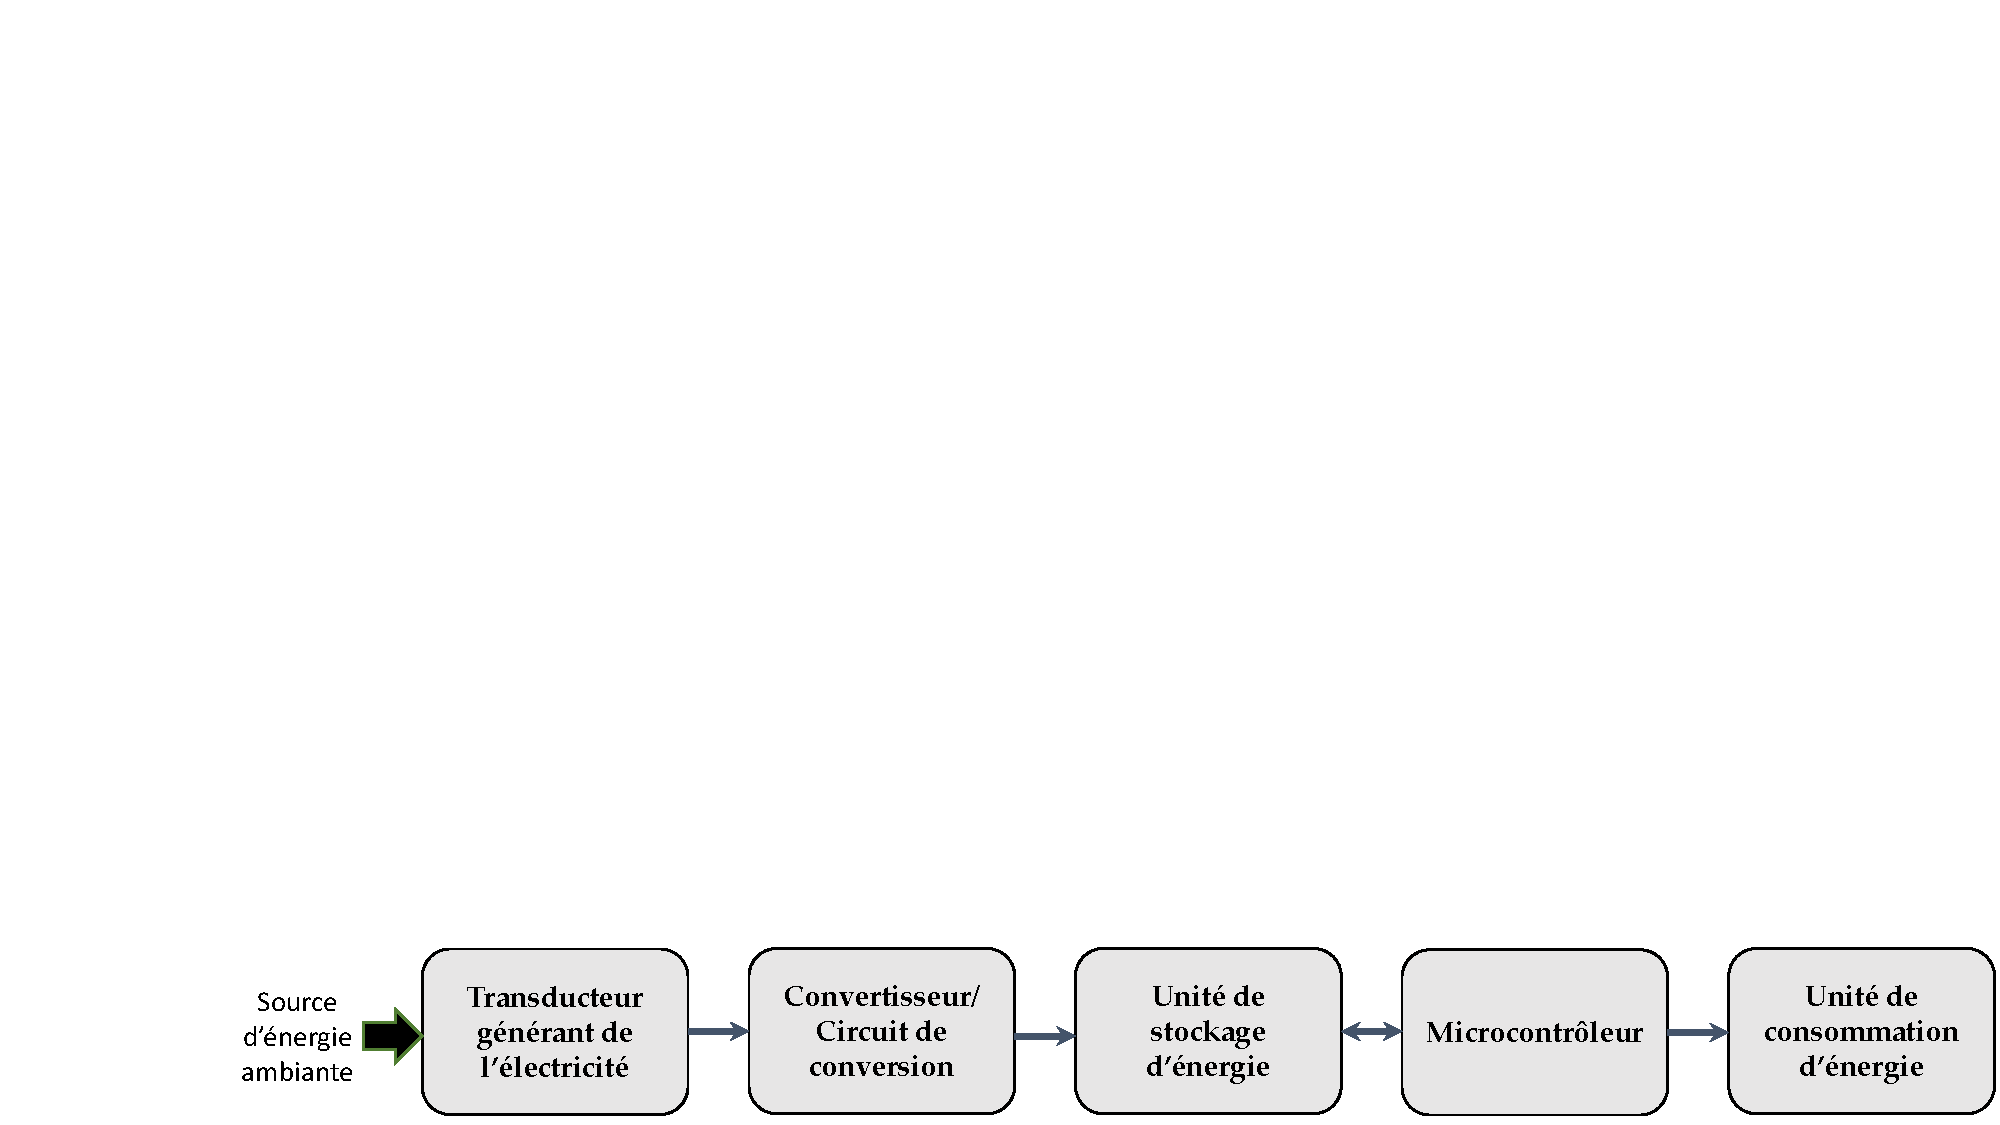
\includegraphics[trim={4cm 0cm 0cm 16cm},clip, width=\textwidth]{../Chap1/Figure/diagramme_bloc_recuperateur.pdf}
		\caption{Diagramme bloc centré sur un système de récupération d'énergie.}
		\label{fig:diagramme_bloc_recuperateur}
	\end{center}
\end{figure}

Les activités du corps humain génèrent un montant considérable d'énergie de différentes natures comme les activités musculaires physiques et chimiques, les mouvements des membres, la marche, les battements du c\oe{}ur, la chaleur corporelle, ou bien encore, la déformation des tissus mous. Une partie de cette énergie est perdue par dissipation. Par conséquent, diverses méthodes de conversion d'énergie ont été développées pour les valoriser. Le tableau \ref{tab:Technos conversion d energie} donne une explication qualitative du fonctionnement des différentes technologies de conversion existantes, ainsi que leurs avantages et inconvénients majeurs.
%%%%%%%%%%%%%%%%%%%%%%%%%%%%%%%%%%%%%%%
\begin{table}[!htbp]
\centering
\resizebox{\textwidth}{!}{%
\begin{tabular}{ m{2.5cm} | m{9cm} | m{3.5cm} | m{3.5cm} }
\toprule
\rowcolor{blue!10}
\textbf{Méthode}		&	\textbf{Description}	 &	\textbf{Avantages}	&	\textbf{Inconvénients}	\\
\midrule
\rowcolor{black!8} 
\mbox{Thermoélectricité}						&%%%%%%%%%%%%%%%%%%%%%%%%%%%%%%%%%%%%%
Les matériaux thermoélectriques permettent de convertir l'énergie thermique en énergie électrique. L'effet Seebeck, à l'origine de ce phénomène, permet la génération de différence de potentiel électrique lorsqu'un gradient de température subsiste entre deux matériaux thermoélectriques.
&	Conformité \mbox{géométrique} élevée, \mbox{miniaturisable} simple, faible coût.	
&	Efficacité de conversion d'énergie faible, développement lent, nécessite une source de chaleur constante. \\ 
Piles \mbox{à combustibles} \mbox{microbiennes}	& %%%%%%%%%%%%%%%%%%%%%%%%%%%%%%%%%%%%%
Aussi appelées biopiles, elles utilisent les bactéries pour convertir directement en électricité une partie de l’énergie disponible dans un substrat biodégradable. Les biopiles peuvent être alimentées par une diversité de molécules organiques simples (sucres, protéine, etc.) ou directement avec des eaux usées à traiter.
& Utilisable dans les applications invasives avec l'oxydation du glucose &	Faible efficacité, durée de vie et densité de puissance. \\
\rowcolor{black!8} 
\mbox{Photovoltaïque}							& %%%%%%%%%%%%%%%%%%%%%%%%%%%%%%%%%%%%%
La cellule photovoltaïque est un matériau, semi-conducteur ou organique, capable de générer de l'électricité à partir de lumière, grâce à l'effet photovoltaïque. Les cellules peuvent être bio-intégrés, mais on les trouve aussi sur des dispositifs nomades non invasifs.
&	Bio-compatibilité, conformité géométrique, miniaturisable.
&	Coût élevé des semi-conducteurs, durée de vie faible des cellules organiques, source d'énergie faible en intérieur, efficacité faible. \\
\mbox{Électro-statisme}							& %%%%%%%%%%%%%%%%%%%%%%%%%%%%%%%%%%%%%
L'électrostatisme consiste à exploiter la variation de capacité d'un système capacitif chargé, afin de produire de l'énergie électrique. On distingue deux familles. La première rassemble les matériaux actifs type électrets, exploitant la variation de capacité créée par variation de distance entre les deux électrodes. La seconde exploite la génération de charges à partir de frottements avec les matériaux triboélectriques. 
& 	Densité de puissance élevée, conformité géométrique, fabrication simple et économique.
&	Tension de fonctionnement élevée, nécessité de polarisation, efficacités faibles, courant de sortie faible. \\
\rowcolor{black!8} 
Induction \mbox{électromagnétique}				& %%%%%%%%%%%%%%%%%%%%%%%%%%%%%%%%%%%%%
L'induction électromagnétique est la génération de courant dans un circuit électrique suite à la variation de champ magnétique générée par le déplacement relatif entre un aimant et celui-dernier.
&	Réalisation simple et faible coût, robuste et durée de vie élevée
&	Miniaturisation difficile, tension de sortie et capacité faible, efficacité faible aux petites échelles \\
\mbox{Piézoélectricité}							& %%%%%%%%%%%%%%%%%%%%%%%%%%%%%%%%%%%%%
La piézoélectricité se produit au sein des matériaux piézoélectriques qui ont la particularité de se polariser électriquement sous l'action d'une contrainte. Deux électrodes inversement polarisées permettent la génération de tension entre leurs bornes respectives.
& Utilisation simple, tension de sortie et capacité élevée
& Fragilité des céramiques piézoélectriques, efficacité faible des polymères piézoélectriques. \\
\bottomrule
\end{tabular}}
\caption{Les technologies de conversion d'énergie et leur pertinence dans le cadre de la récupération d'énergie sur le corps humain}
\label{tab:Technos conversion d energie}
\end{table} 
%%%%%%%%%%%%%%%%%%%%%%%%%%%%%%%%%%%%%%

Le tableau \ref{tab:Technologies de recuperation d'energie sur le corps humain} rassemble par ailleurs quelques exemples de  sources d'énergie disponibles autour du corps humain, ainsi que les technologies de récupération d'énergie mises en \oe{}uvre pour leur grappillage. Des articles de synthèse récents donnent de nombreux d'exemples supplémentaires \cite{Khalid2019,Kumari2020}. Les densités énergétiques récupérables sur le corps humain se situent généralement dans l'ordre de grandeur du microwatt par unité de surface ou bien par unité de volume, quelle que soit la technologie de conversion envisagée. La notion de densité est par ailleurs relativement vague dans la littérature lorsqu'elle concerne la récupération. En effet, un dispositif, dès lors qu'il est encapsulé, voit généralement ses performances diminuer (réduction de 22$\micro$W/cm$^3$ à 2.82$\micro$W/cm$^3$ pour \cite{Azimi2021}). De plus, les définitions du volume efficace du dispositif et de l'environnement de test restent parfois discutables. Néanmoins, l'ordre de grandeur des puissances récupérables est comparable aux consommations des divers appareils nomades dans l'environnement du corps humain, comme, un stimulateur cardiaque moderne qui nécessite une puissance de 0.3$\micro$W pour un fonctionnement normal \cite{Kumari2020}.
%%%%%%%%%%%%%%%%%%%%%%%%%%%%%%%%%%%%%%
\begin{table}[!htbp]
\centering
\resizebox{\textwidth}{!}{%
\begin{tabular}{ l l m{7cm} l}
\toprule
\rowcolor{blue!10}
\textbf{Source d'énergie} 	& \textbf{Méthode de transduction}	& \textbf{Applications} & \textbf{Densité de puissance}	\\	 
\midrule
%%%%%%%%%%%%%%%%
\rowcolor{black!8} 
Chaleur corporelle			&	Thermoélectricité				&
Capteurs autonomes cutanés \cite{Kim2014}						& 15$\micro$W/cm$^3$ à \ang{15}C ambiant \\	
%%%%%%%%%%%%%%%%
Lumière ambiante			&	Photovoltaïque					&
Dispositifs sous cutanés \cite{Zhao2020}						& 4$\micro$W/cm$^2$  \\			
%%%%%%%%%%%%%%%%
\rowcolor{black!8} 
Glucose						& 	Biopile enzymatique 			&
Dispositifs sous-cutanés	\cite{Wang2009}						& [0.3-1.38]$\micro$W/cm$^2$ \\	
%%%%%%%%%%%%%%%%
Déformation tissus			&Électromagnétique/piézoélectrique	&
Dispositifs nomades déformables  \cite{Kwon2017}				& NA \\						
%%%%%%%%%%%%%%%%
\rowcolor{black!8} 
Marche						&	Céramiques piézoélectriques		&
Électronique pour un implant de genou \cite{Almouahed2016}		& NA \\
%%%%%%%%%%%%%%%%
Marche						&	Électro-statisme (variation de distance + triboélectricité)				&
Dispositifs nomades \cite{Yang2013}								& 3$m$W/cm$^2$ \\	
%%%%%%%%%%%%%%%%
\rowcolor{black!8} 																	
Marche						&	Triboélectricité 				&
Simulateur cardiaque auto-rechargeable \cite{Ryu2021}						& 4.9$\micro$W/cm$^3$\\
%%%%%%%%%%%%%%%%
Battements cardiaques		 &	Polymère piézoélectrique		&
Simulateur cardiaque auto-rechargeable \cite{Azimi2021}					& 2.82$\micro$W/cm$^3$ \\
%%%%%%%%%%%%%%%%
\bottomrule
\end{tabular}}
\caption{Technologies de récupération d'énergie sur le corps humain}
\label{tab:Technologies de recuperation d'energie sur le corps humain}
\end{table} 
%%%%%%%%%%%%%%%%%%%%%%%%%%%%%%%%%%%%%%%

Des défis majeurs sont cependant inhérents au contexte applicatif peu commun qu'est le corps humain.

Les générateurs thermoélectriques sont capables de prendre des formes géométriques complexes et constituent de ce fait une solution intéressante pour l'exploitation de la chaleur constante produite naturellement par le corps humain. Cependant, malgré leur longue durée de vie et leur grande fiabilité, ces dispositifs souffrent de coûts élevés et d'une faible efficacité de conversion liée à la nécessité de gradients de température importants et continus.

Les convertisseurs triboélectriques se démarquent sur une majorité des solutions d'alimentations alternatives des appareils nomades cutanés et sous-cutanés grâce à leur forte densité de puissance, forte efficacité de conversion et leur conformité géométrique à très faible échelle. Ils sont cependant désavantagés par leur durabilité et leur robustesse, ainsi que leur comportement physique parfois difficile à prédire à cause des lacunes de compréhension dans le domaine. Cette solution est néanmoins couramment étudiée, car elle présente l'avantage d'être facilement intégrable pour les applications sous-cutanés \cite{Ryu2021}.

Les convertisseurs électromagnétiques sont des dispositifs générant un maximum de puissance lorsque la source d'excitation externe est synchronisée avec leur fréquence de résonance propre \cite{Razek2020}. Cette caractéristique est d'ailleurs vraie pour tous les systèmes à conversion mécano-électrique. La récupération sur une large bande de fréquences est difficile à atteindre sur les générateurs électromagnétiques à l'échelle de dispositifs bio-intégrables. Ils sont de ce fait rarement utilisés, car les déformations mécaniques et les mouvements du corps humain sont lents et généralement acycliques. De surcroît, les faibles tensions de sortie des générateurs électromagnétiques rendent leur redressement difficile.

Les céramiques piézoélectriques se démarquent par leur tension de sortie élevée et leur fort coefficient de couplage électromécanique, mais leur bio-intégration est complexe à cause de leur rigidité importante. Les polymères piézoélectriques sont des matériaux composites constitués d'un mélange de résine et de céramiques. Ils peuvent être une approche intéressante pour améliorer l'intégrabilité de cette solution de conversion, mais leur coefficient de couplage électromécanique est inversement proportionnel à leur souplesse. Les générateurs piézoélectriques en céramiques, comme les générateurs électromagnétiques, sont généralement des éléments résonnants et leur puissance de sortie est donc d'autant plus importante que leur fréquence est proche de l'excitation externe.

L'énergie de déformation mécanique des tissus mous, ainsi que l'énergie cinétique liée aux mouvements des différentes parties du corps, sont les sources d'énergie prépondérantes sur le corps humain. Cela motive d'autant plus le développement des technologies de conversion électromécaniques. On constate cependant que la faible fréquence de ces sources constitue un frein pour l'efficacité de production d'énergie des transducteurs électromécaniques conventionnels. De plus, le caractère mou des tissus humains rend difficile l'intégration directe d'interfaces mécaniques rigides pour la captation de l'énergie. Des solutions sont proposées dans la littérature pour l'amélioration des rendements de conversion des récupérateurs d'énergie électromécaniques, ainsi que pour l'amélioration de leur bio-intégrabilité.
    %////////////////////////////////////////////
	\subsection{Solutions technologiques pour l'amélioration des récupérateurs électromécaniques}
	\label{subsec:1.3.4_Solutions technologiques pour l amelioration des recuperateurs}
	%////////////////////////////////////////////
Un travail important a été réalisé au cours des dernières années pour améliorer les systèmes de récupération d'énergie mécanique en utilisant les différents types de transduction présentés, combinés à de nombreuses techniques d'optimisation et de conception. Ces approches ont été étudiées théoriquement et mises en \oe{}uvre expérimentalement pour tirer parti, autant que possible, des excitations externes en maximisant l'énergie récoltée. En considérant une source unidirectionnelle, on retrouve deux méthodes d'optimisation majeures que sont la récupération d'énergie large bande et la conception de systèmes non résonnants.

L'élargissement de la bande passante des récupérateurs d'énergie électromécaniques vise à améliorer la réponse du système face à la source. Elle peut être obtenue par les moyens suivants :
\begin{itemize}[label=$\circ$]
	\item Régler la fréquence du système en modifiant les paramètres géométriques \cite{Jang2011} ou bien sur le paramètre de masse \cite{Karadag2017}. Ces techniques permettent d'ajuster la fréquence de résonance du système sans impacter son amortissement. Cependant, cette approche de réglage est très difficile à appliquer aux systèmes de récupération basés sur les microsystèmes électro mécaniques (\emph{MEMS en anglais}), mis à part pour les applications électrostatiques.
	\item Régler la fréquence du système en appliquant une raideur négative par le biais de systèmes piézoélectriques, électrostatiques, ou bien électromagnétiques additionnels. La dernière a cependant le désavantage de complexifier les systèmes en rendant difficile leur intégration \cite{Tang2013,Yildirim2017}.
   	\item Exploiter les éléments piézoélectriques sur leur mode 33, plutôt que le 31 \cite{Morris2008}. Cela se fait notamment grâce à des structures de type flextenseur, capables de transmettre des efforts dans une direction orthogonale à celle de leur provenance.
    \item Utiliser des systèmes à multifréquence de résonance, composés de l'assemblage de plusieurs sous-systèmes de fréquences propres différentes, comme des poutres piézoélectriques de dimensions différentes \cite{Sari2008}.
    \item Utiliser des systèmes à réponse fréquentielle multimodale. Ils sont généralement composés de plusieurs masses dynamiques \cite{Toyabur2018}.
\end{itemize}
%%%%%%%%%%%%%%%%%%%%%%%%%%
\begin{figure}[!htbp]
	\begin{center}
		\captionsetup{justification=centering}
		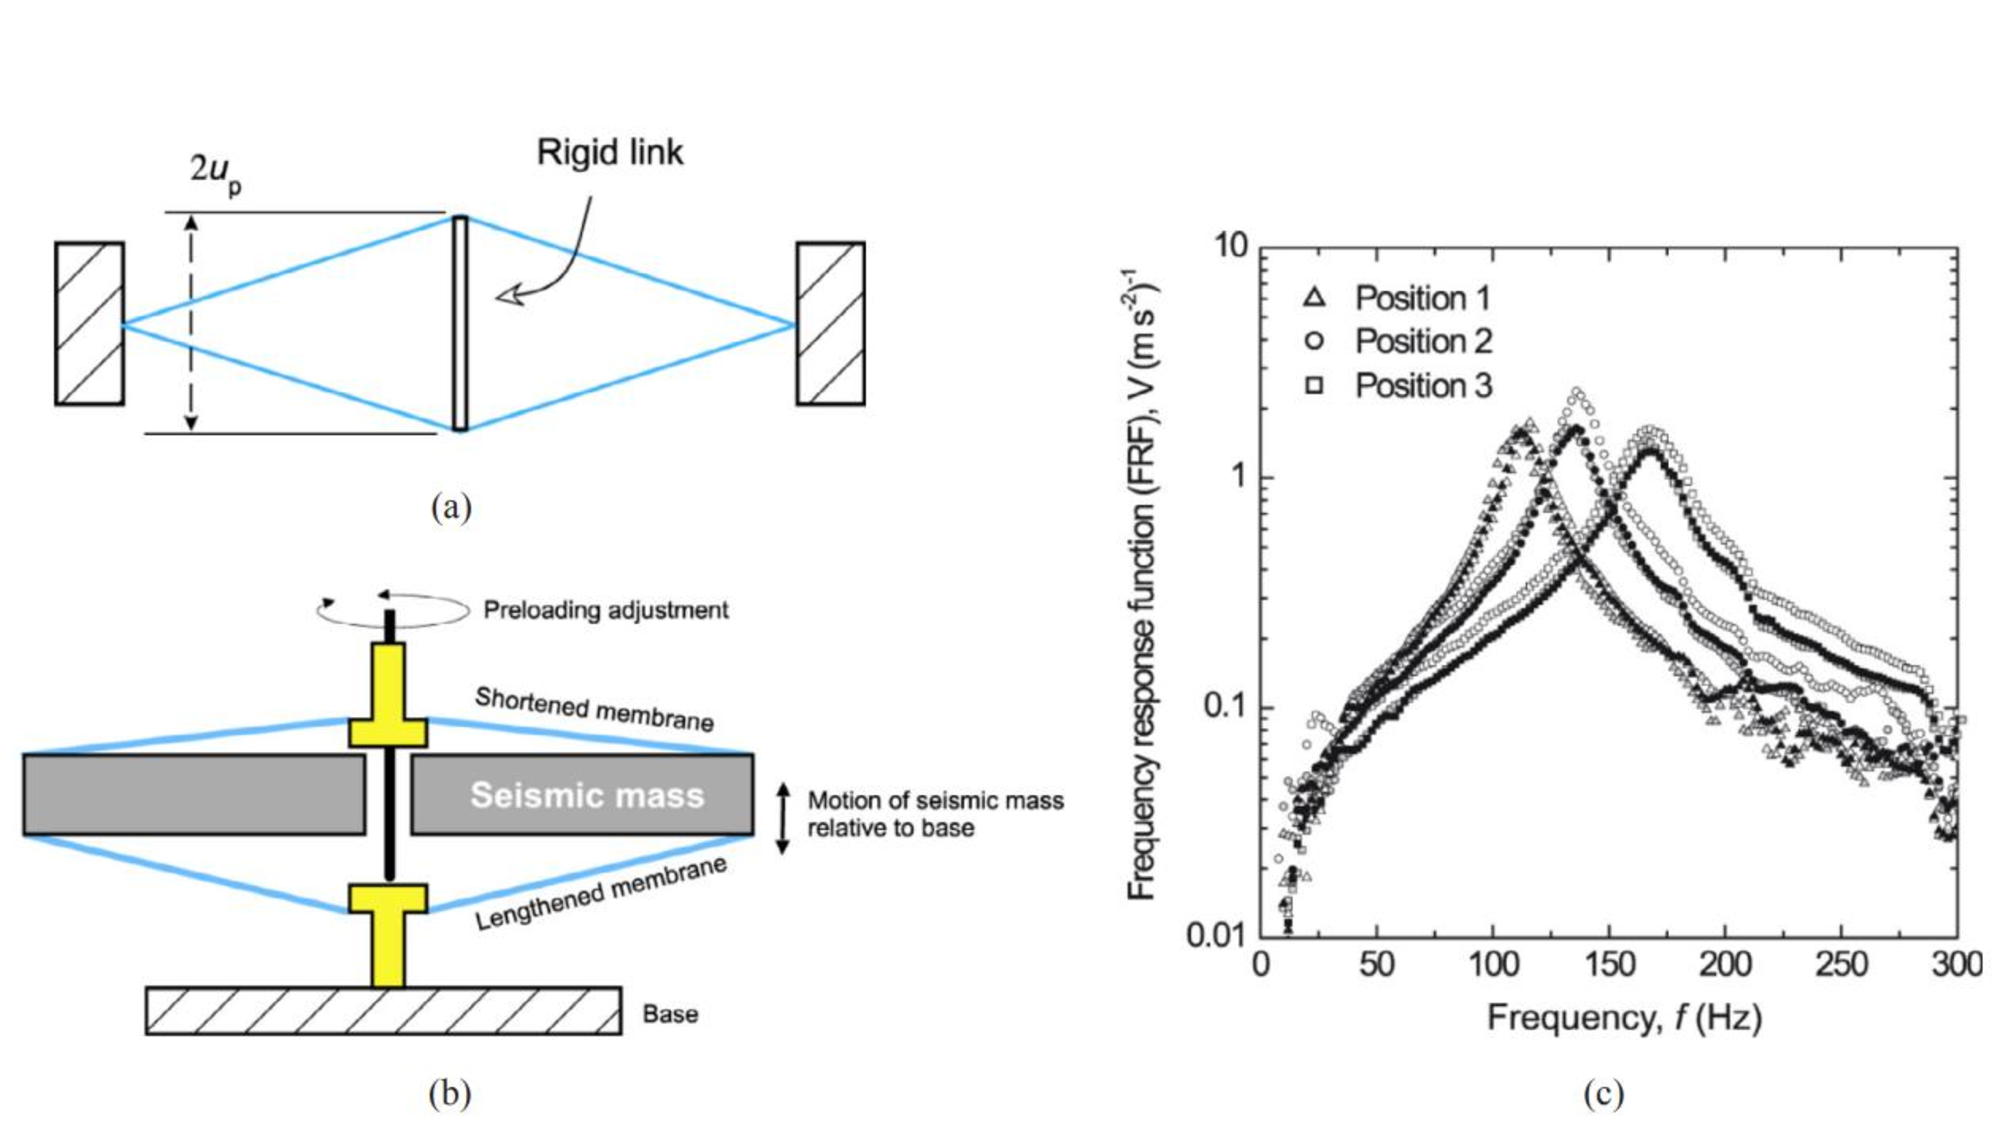
\includegraphics[trim={0cm 0cm 0cm 2cm},clip,width=0.8\textwidth]{../Chap1/Figure/flextenseur.pdf}
		\caption{Récupérateur piézoélectrique accordable en fréquence proposé par Morris \emph{et al.} \cite{Morris2008}: (a) Concept de base (sans masse sismique), (b) Schéma en coupe transversale lorsqu'entraîné par une excitation de la base(c) Réponse fréquentielle pour différentes positions de précontrainte initiale.}
		\label{fig:flextenseur}
	\end{center}
\end{figure}
%%%%%%%%%%%%%%%%%%%%%%%%%%	
Des articles de synthèses présentent d'autres méthodes supplémentaires répondant à la problématique, tels que le réglage actif en fréquence au moyen de circuits d'extraction non linéaires dans le cas des systèmes fortement couplés, ou bien la récupération large bande au moyen d'oscillateurs bistables \cite{Yildirim2017,Maamer2019}. Ces méthodes sont utiles dans le cadre de la récupération d'énergie à partir de sources ambiantes vibratoires (fréquence supérieure à 50Hz). L'énergie générée par l'activité humaine est cependant de fréquence faible (inférieure à 10Hz), voire acyclique. Il est alors pertinent de relever les solutions de développements de systèmes de récupérations de sources non résonantes. Ces-derniers peuvent être obtenus par les moyens suivants :
\begin{itemize}[label=$\circ$]	% LTeX: language=fr
	\item La conversion \emph{frequency-up} classique permettant d'amplifier la fréquence de la source d'énergie. Elle combine un système basse fréquence (BF) et un autre haute fréquence (HF). L'excitation externe est captée par le système BF, puis transférée au système HF pour la phase de conversion en électricité. Une amplitude importante est cependant nécessaire afin que l'interaction entre les deux systèmes puisse avoir lieu. Cette méthode est adaptée aux convertisseurs électromagnétiques, comme aux convertisseurs piézoélectriques. Les figures \ref{fig:frequency-up electromag} et \ref{fig:frequency-up piezo} montrent respectivement deux exemples de mécanismes \emph{frequency-up} pour des récupérateurs électromagnétiques et deux pour des récupérateurs piézoélectriques. Cette méthode d'optimisation des systèmes de récupération induit généralement du frottement au contact des deux systèmes BF et HF. Cela affecte le rendement de conversion et peut amener une usure prématurée des dispositifs et réduire ainsi leur durée de vie. Des solutions ingénieuses impliquant l'utilisation de systèmes mécaniques bistables comme absorbeur BF permettent de s'affranchir de ces frottements \cite{Galchev2009}.
	\item La conversion \emph{frequency-up} à bille libre permettant de récupérer l'énergie générée par la collision entre un objet en mouvement libre (système BF) et le système HF. Un exemple d'application est proposé par Halim \emph{et al.} et illustré sur la figure \ref{fig:frequency-up free_ball} \cite{Halim2015}.
\end{itemize}
%%%%%%%%%%%%%%%%%%%%%%%%%%
\begin{figure}[!htbp]
	\begin{center}
		\captionsetup{justification=centering}
		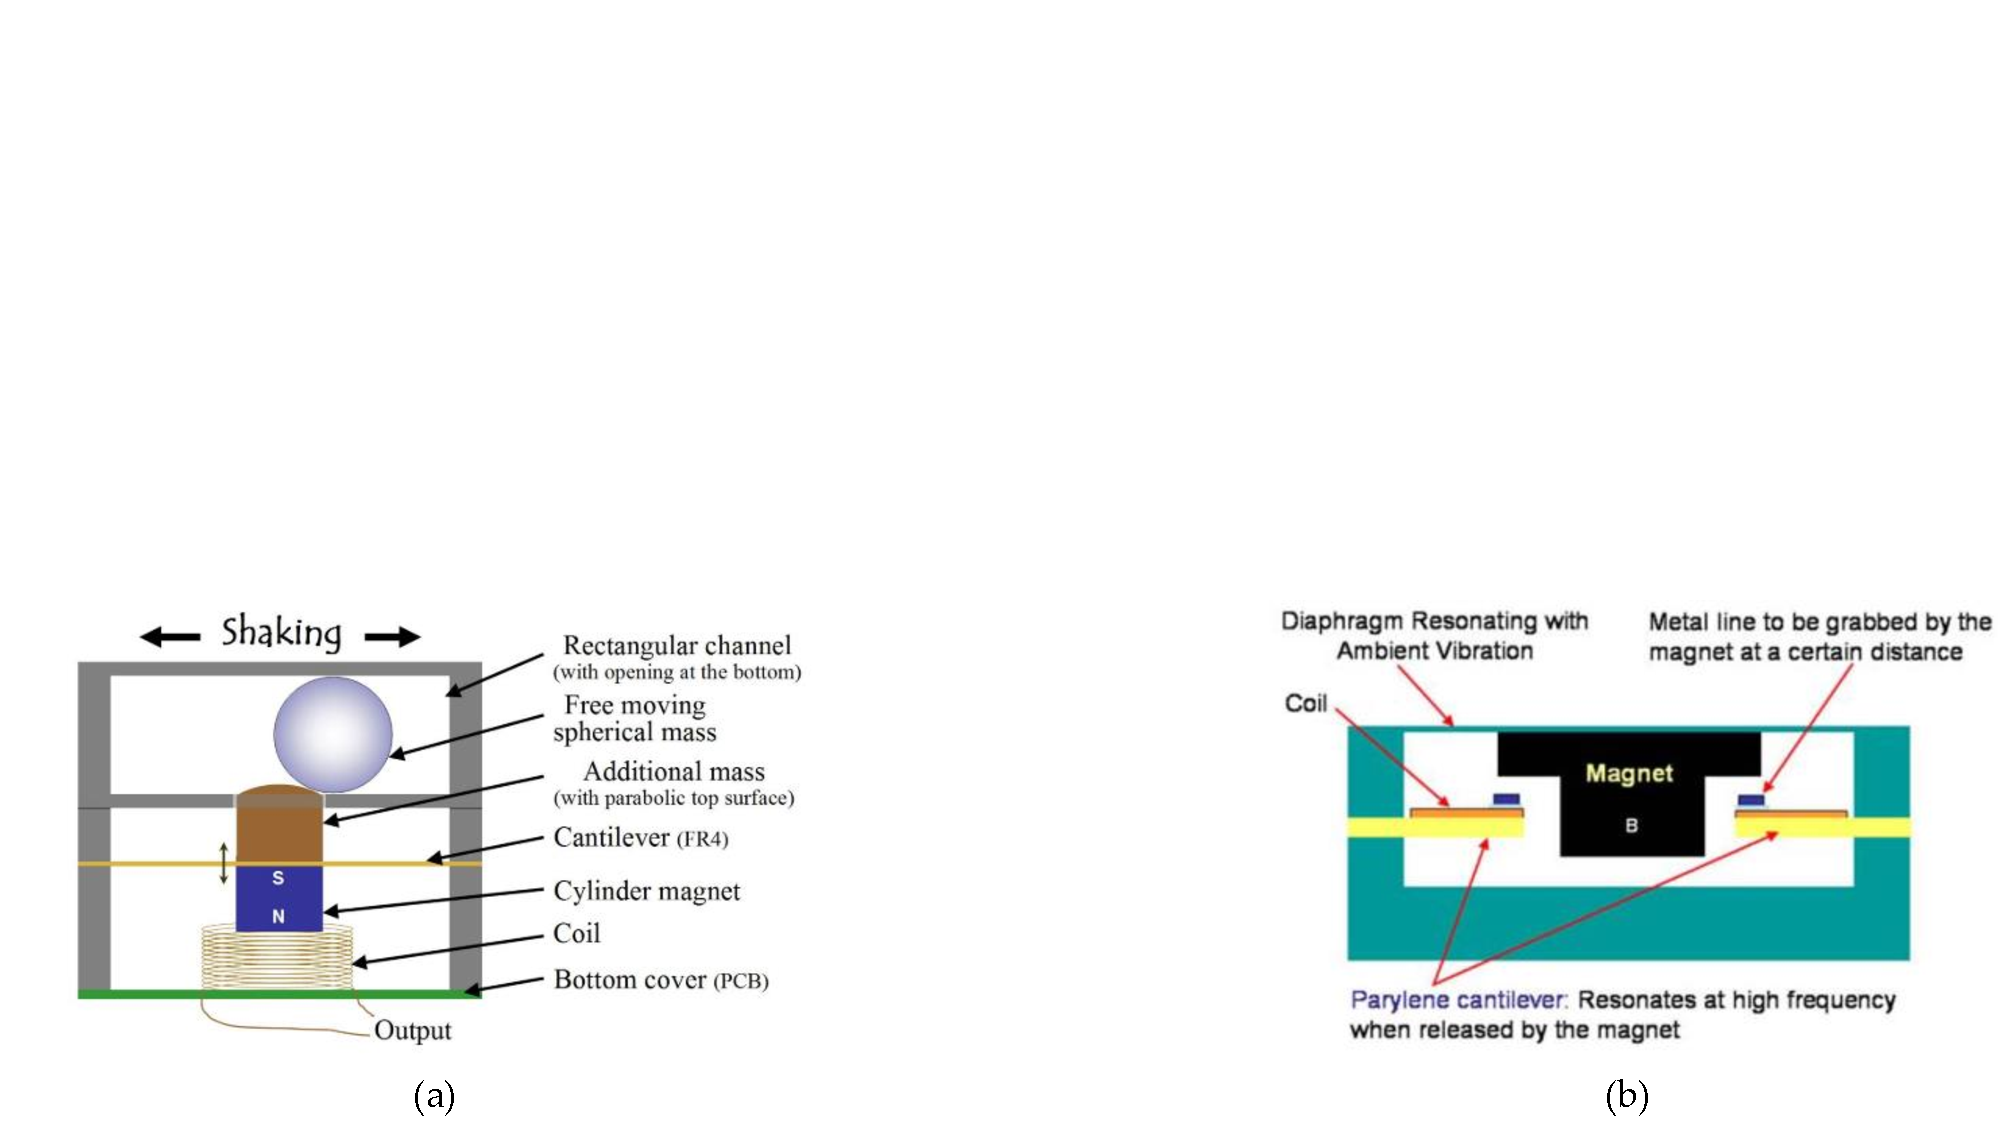
\includegraphics[trim={1cm 0cm 0cm 10cm},clip, width=\textwidth]{../Chap1/Figure/frequency-up_EM.pdf}
		\caption{Exemples de mécanismes de conversion \emph{frequency-up} pour des générateurs électromagnétiques. (a) \cite{Halim2013}, (b) \cite{Sari2010}}
		\label{fig:frequency-up electromag}
	\end{center}
\end{figure}
%%%%%%%%%%%%%%%%%%%%%%%%%%
%%%%%%%%%%%%%%%%%%%%%%%%%%
\begin{figure}[!htbp]
	\begin{center}
		\captionsetup{justification=centering}
		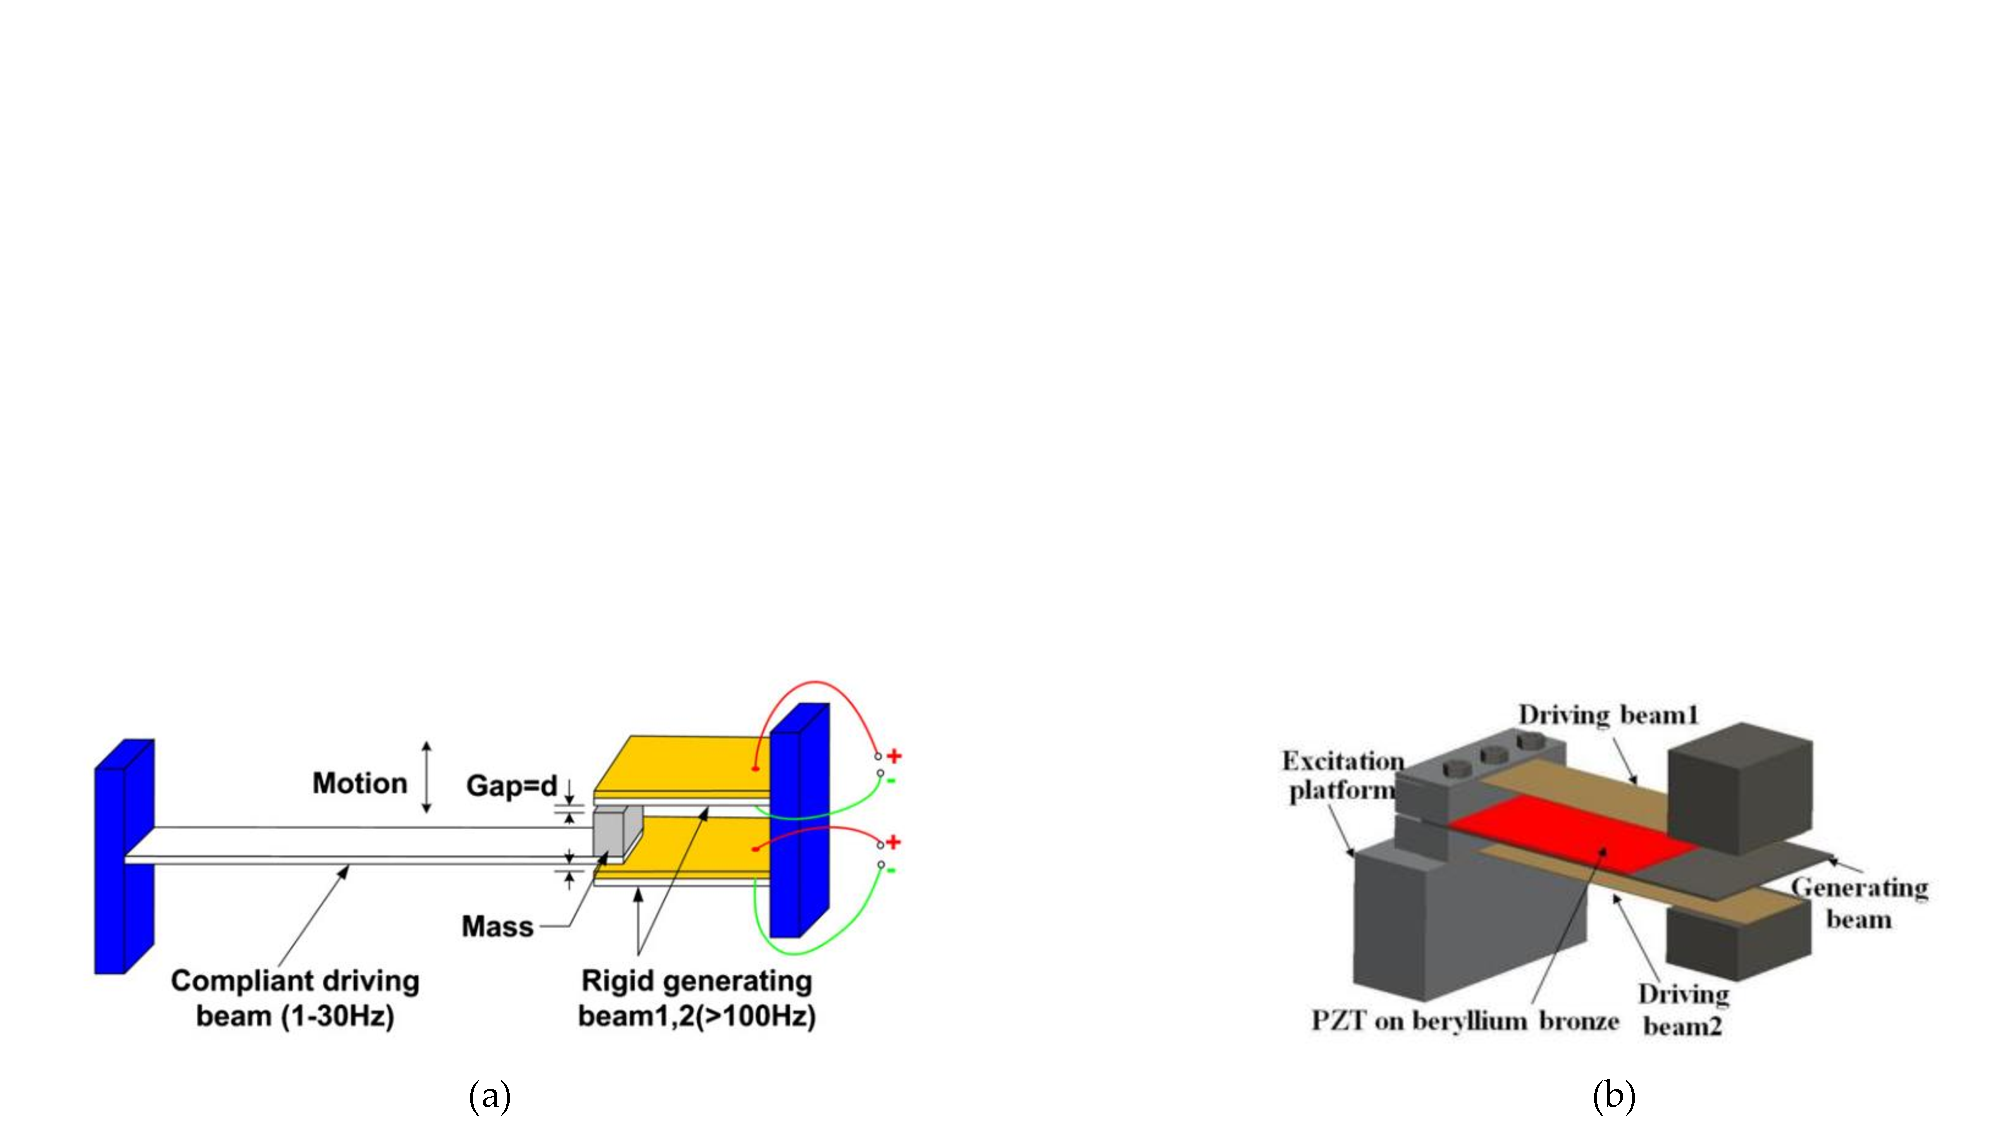
\includegraphics[trim={1cm 0cm 0cm 10cm},clip, width=\textwidth]{../Chap1/Figure/frequency-up_piezo.pdf}
		\caption{Exemples de mécanismes de conversion \emph{frequency-up} pour des générateurs piézoélectriques. (a) \cite{Gu2011}, (b) \cite{Zhang2018}}
		\label{fig:frequency-up piezo}
	\end{center}
\end{figure}
%%%%%%%%%%%%%%%%%%%%%%%%%%
%%%%%%%%%%%%%%%%%%%%%%%%%%
\begin{figure}[!htbp]
	\begin{center}
		\captionsetup{justification=centering}
		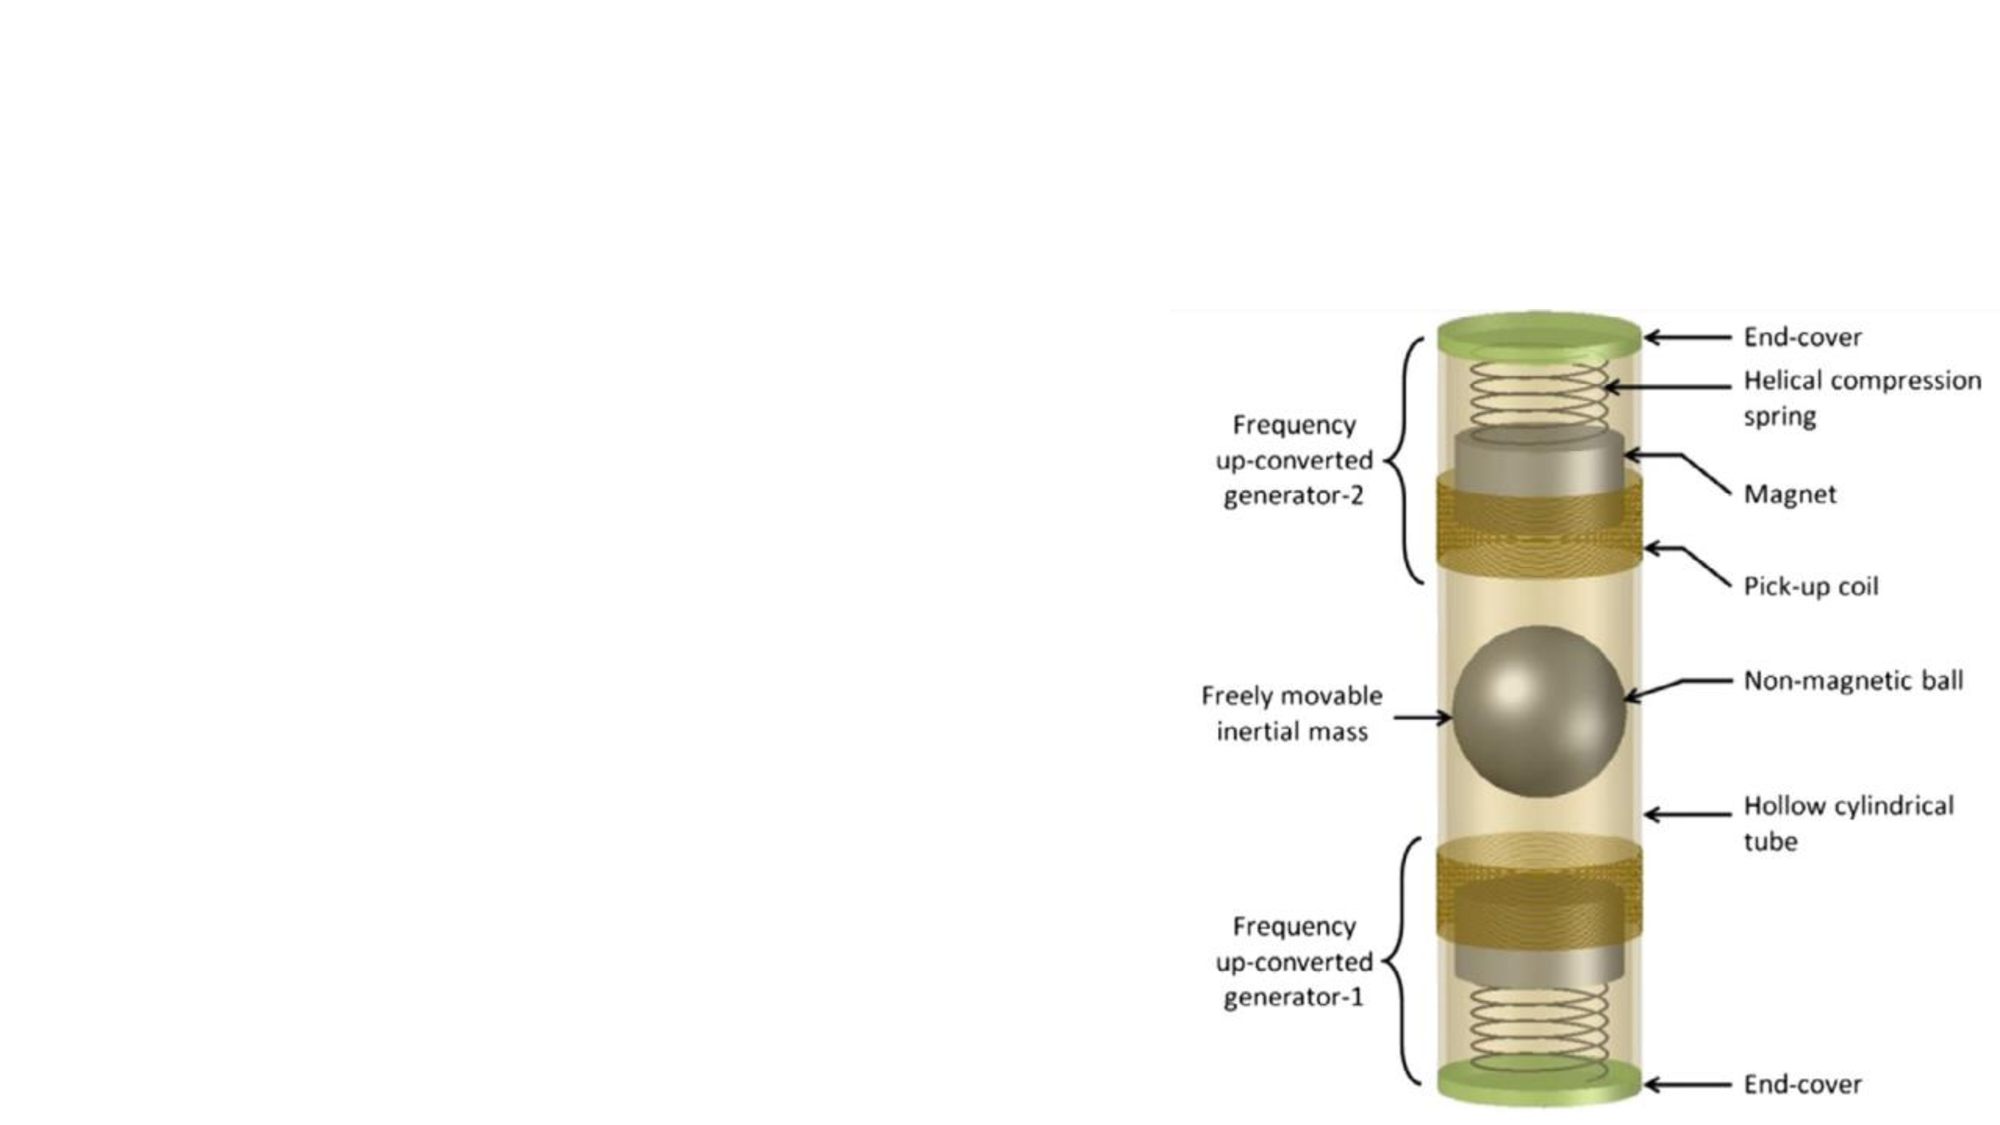
\includegraphics[trim={20cm 0cm 0cm 5cm},clip, width=0.5\textwidth]{../Chap1/Figure/free_ball.pdf}
		\caption{Exemples de mécanismes de conversion \emph{frequency-up} à bille libre \cite{Halim2015}}
		\label{fig:frequency-up free_ball}
	\end{center}
\end{figure}
%%%%%%%%%%%%%%%%%%%%%%%%%%

L'optimisation des systèmes de récupération d'énergie piézoélectriques et électromagnétique présente une grande variété de solutions dont les quelques exemples pertinents ont été énoncés dans cette section. La solution piézoélectrique est celle qui semble privilégiée dans la littérature, offrant la meilleure approche pour l'exploitation de l'énergie mécanique sur le corps humain. Cet aspect sera développé plus en détail dans la section \ref{subsec:1.4.3_Etat de l art sur les recuperateurs existants}. De plus, les techniques \emph{frequency-up} classiques implémentant un système BF absorbeur et un système HF convertisseur sont les choix d'améliorations de performances les plus récurrents grâce à leur conception simple et leur réponse large bande. Ils présentent cependant le désavantage d'implémenter des pièces d'usure et nécessitent un volume total plus important qu'une majorité de récupérateurs non optimisés. Leur utilisation sera pertinente dans les applications allouant un volume de travail conséquent, typiquement, les appareils auditifs ou bien les implants cochléaires.

    %////////////////////////////////////////////
	\subsection{Synthèse sur la récupération d'énergie sur le corps humain}
	\label{subsec:1.3.5_Synthese sur la recuperation d energie sur le corps humain}
	%////////////////////////////////////////////

Le besoin énergétique a été mis en évidence pour les applications nomades autour et dans le corps humain. La consommation énergétique des dispositifs les plus récents est optimisée au travers d'architectures et technologies favorisant le fonctionnement à faible puissance. Ces améliorations sont développées avec l'optique de ne pas altérer la bio-intégrabilité du système. Lorsque les limites de l'optimisation de la consommation énergétique sont atteintes, il est possible de se tourner vers les technologies de récupération de l'énergie naturellement dissipée par les activités du corps humain. Différentes sources d'énergie y subsistent et ont été mises en évidence dans cette section. De nombreuses technologies de récupération d'énergie sont proposées dans la littérature pour exploiter l'énergie du corps humain et permettent, dans certains cas, d'atteindre l'autonomie énergétique pour les applications peu énergivores. L'énergie disponible en plus grande quantité sur le corps humain est de source mécanique, ce qui explique la diversité importante dans les familles de récupérateurs électrostatiques, piézoélectriques et électromagnétiques. Les avantages et inconvénients de chacune d'elles ont été soulignés et les récupérateurs piézoélectriques montrent les résultats les plus intéressants pour les applications miniaturisées. La littérature propose aussi différentes méthodes d'optimisation pour amplifier les performances des récupérateurs électromécaniques. Ceux-ci consistent notamment en l'élargissement de la bande fréquentielle de réponse du système de récupération, ou bien en l'augmentation de la fréquence de l'énergie source par le biais du couplage de sous-systèmes BF et HF pour l'exploitation de sources d'énergie acycliques et/ou BF (inférieur à 10Hz).

Dans la suite des travaux, nous allons nous intéresser au cas particulier de la récupération d'énergie dans le conduit auditif pour l'alimentation des appareils nomades intra-auriculaires tels que les appareils auditifs ou bien les implants cochléaires.
%/!\/!\/!\/!\/!\/!\/!\/!\/!\/!\/!\/!\/!\/!\/!\/!\/!\/!\/!\/!\/!\/!\/!\/!\%	
\section{Cas particulier de la récupération d’énergie dans le conduit \mbox{auditif}}
\label{sec:1.4_Cas particulier de la recuperation d energie dans le conduit auditif}
%/!\/!\/!\/!\/!\/!\/!\/!\/!\/!\/!\/!\/!\/!\/!\/!\/!\/!\/!\/!\/!\/!\/!\/!\%.
    %/////////////////////////////////////////////
	\subsection{Caractérisation du besoin}
	\label{subsec:1.3.1_Caracterisation la source d energie}
	%////////////////////////////////////////////
Le développement constant des appareils d'aide à l'audition a donné lieu à des améliorations considérables dans les fonctionnalités et les consommations énergétiques des appareils auditifs et des implants cochléaires. Deux des dispositifs commerciaux les plus courants sont présentés sur la figure \ref{fig:appareils_commerciaux}. La gamme de puissance requise pour leur fonctionnement, ainsi que la consommation énergétique moyenne sur un cycle de 12 heures sont extraites de leurs documentations techniques respectives et listées dans le tableau \ref{tab:appareils_commerciaux_conso}.
%%%%%%%%%%%%%%%%%%%%%%%%%
\begin{table}[!htbp]
	\begin{minipage}[c]{0.5\textwidth}
		\begin{figure}[H]
			\begin{center}
				\begin{subfigure}[t]{0.49\textwidth}
					\captionsetup{justification=centering}
					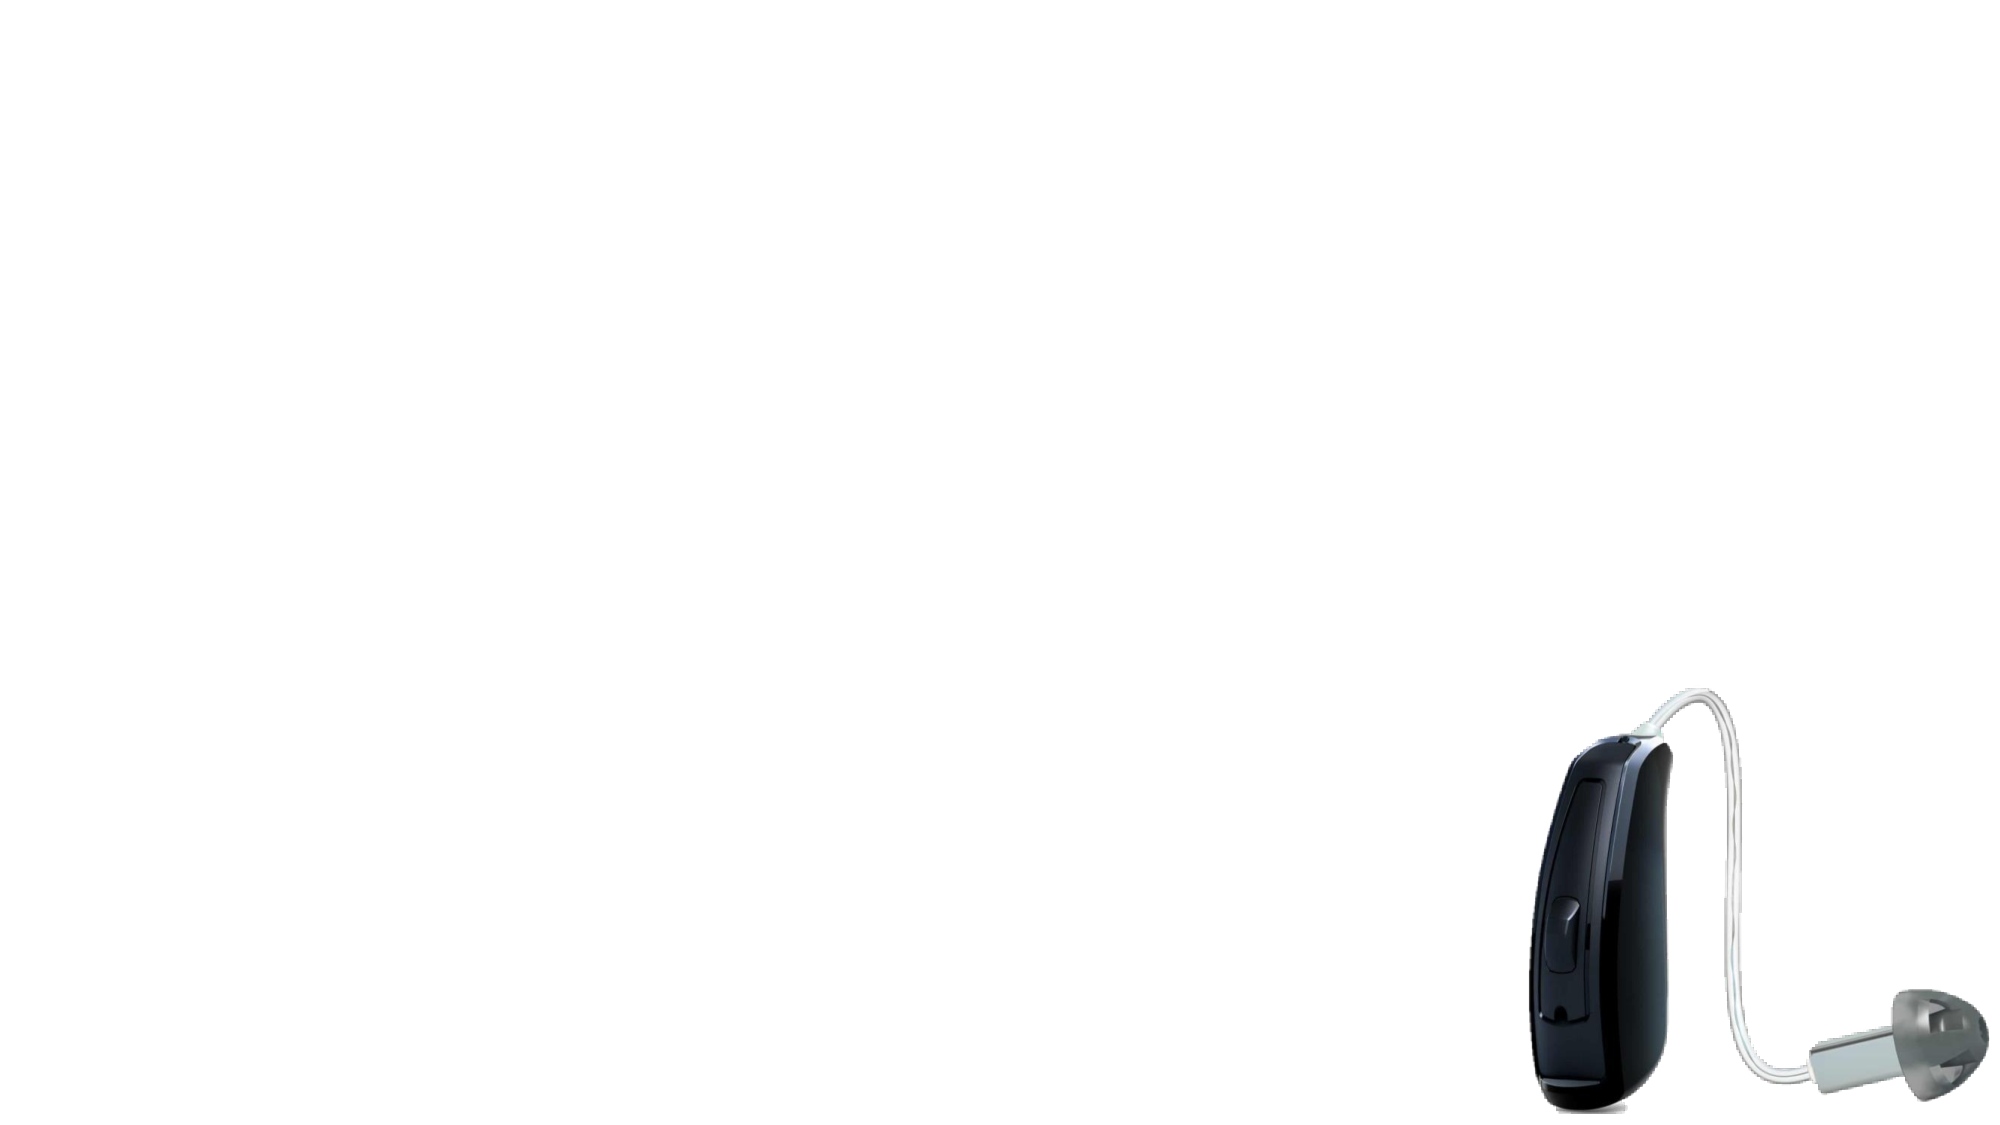
\includegraphics[trim={25cm 0cm 0cm 11cm},clip,width=\textwidth]{../Chap1/Figure/hearing_aid_Resound.pdf}
					\caption{Appareil auditif LYNX Quattro \cite{Quattro2019}}
					\label{fig:hearing_aid_Resound}
				\end{subfigure}
				\hfillx
				\begin{subfigure}[t]{0.49\textwidth}
					\captionsetup{justification=centering}
					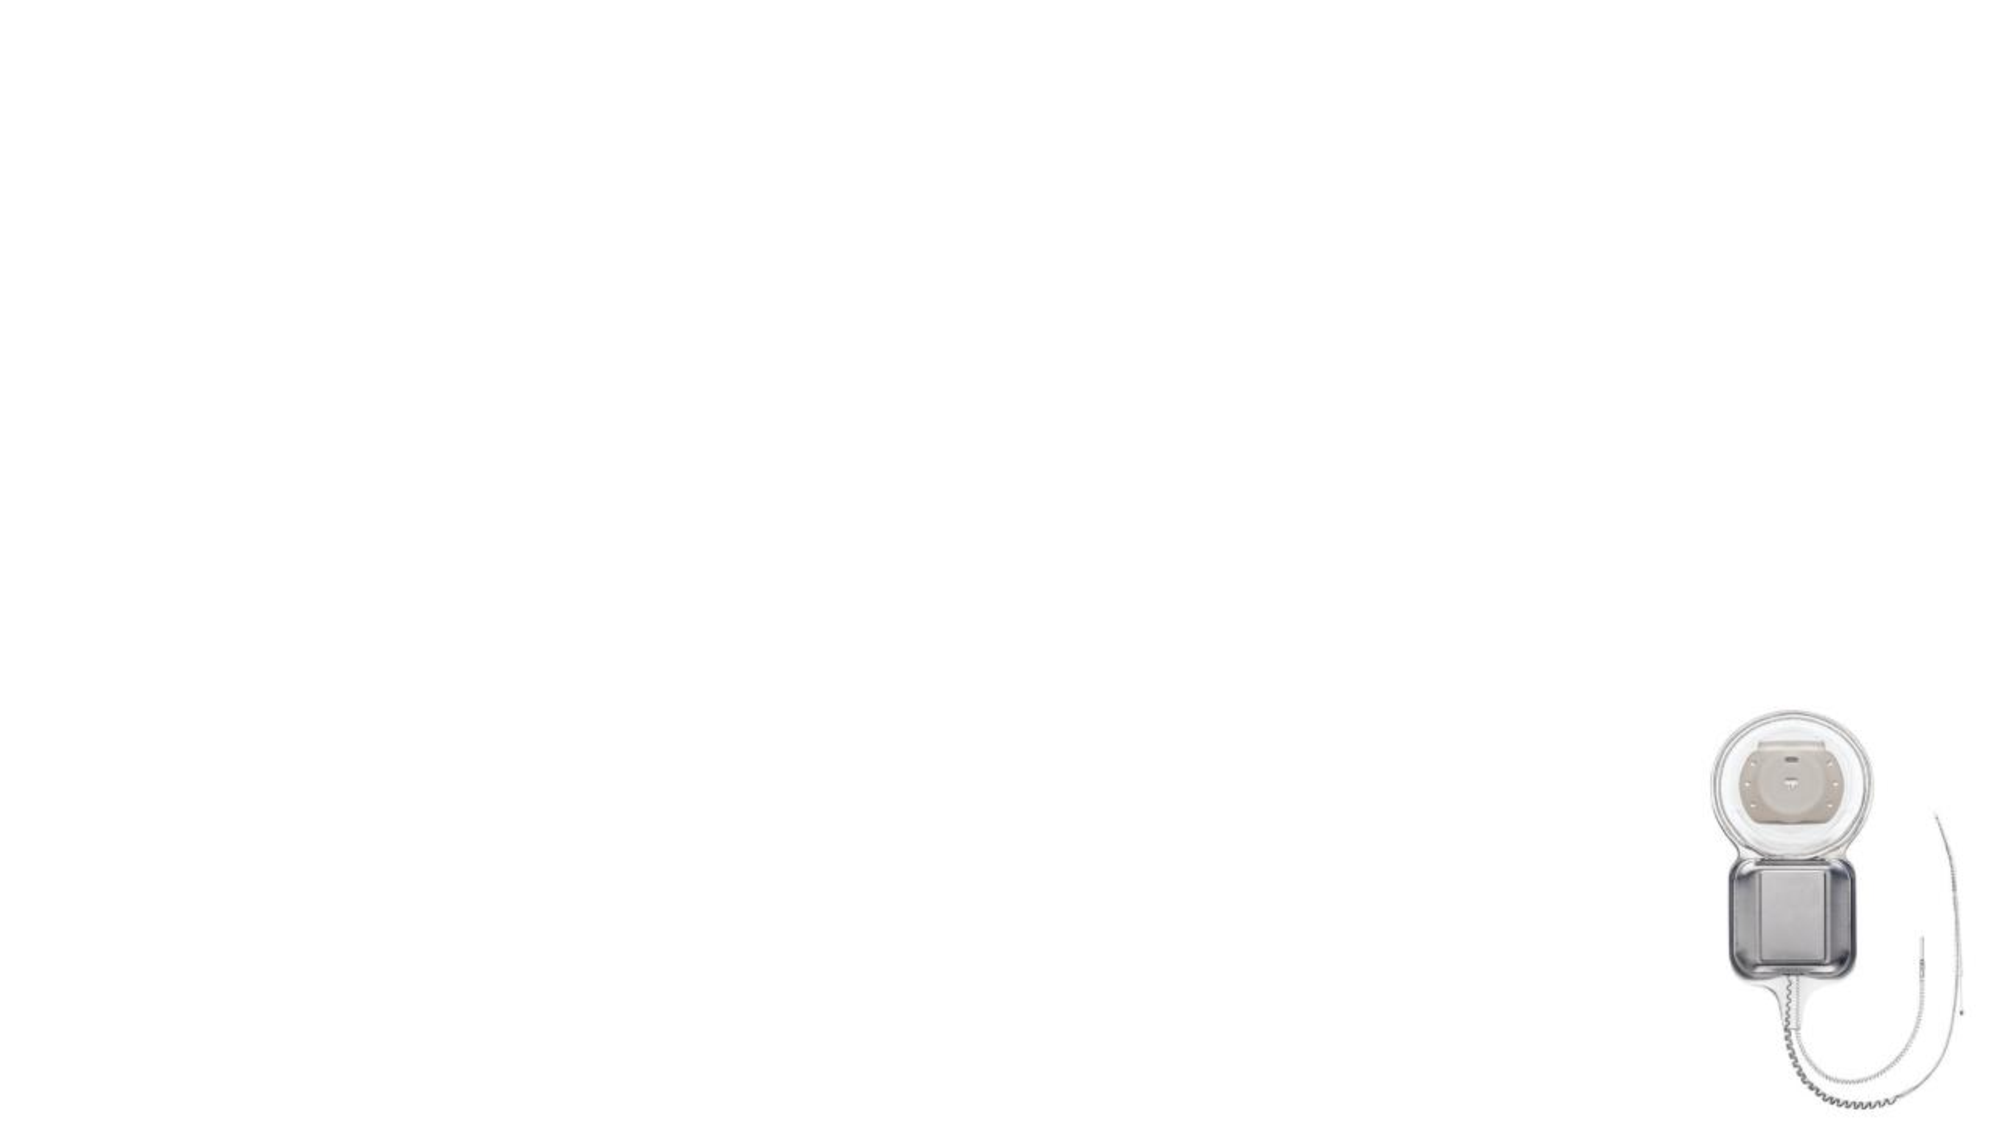
\includegraphics[trim={27cm 0cm 0cm 12cm},clip,width=\textwidth]{../Chap1/Figure/nucleus_Cochlear.pdf}
					\caption{Implant cochélaire Nucléus C1612 \cite{COCHLEAR}}
					\label{fig:implant_Cochlear}
				\end{subfigure}
				\caption{Appareils d'aide à l'audition \mbox{commerciaux}}
				\label{fig:appareils_commerciaux}
			\end{center}
		\end{figure}
	\end{minipage}
	%%%%%%%%%%%%%%%%
	\hfillx
	\begin{minipage}[c]{0.4\textwidth}
		\resizebox{\textwidth}{!}{%
			\begin{tabular}{ l l l}
				\toprule
				\rowcolor{blue!10}
				\textbf{Réf.}       & \textbf{Puissance} & \textbf{Énergie sur 12h} \\
				\midrule
				\rowcolor{black!8}
				\cite{Quattro2019}  & [1-10]mW           & [43-430]J                \\
				\cite{COCHLEAR} & [1.5-2]mW          & [65-87]J                 \\
				\bottomrule
			\end{tabular}}
		\caption{Consommation énergétique des appareils commerciaux}
		\label{tab:appareils_commerciaux_conso}
	\end{minipage}
\end{table}
%%%%%%%%%%%%%%%%	

Ces dispositifs sont très complets et intègrent des fonctions de communication wifi et/ou Bluetooth pour le confort de l'utilisateur. Ces protocoles sont cependant très énergivores d'après les constats précédents et consomment une part considérable de l'énergie fournie par l'unité de stockage. Les fonctions primaires de ces appareils sont la captation du son ambiant et la génération de signaux physiques dans l'oreille. La littérature propose des solutions à bas coût énergétique afin de satisfaire ces derniers. 

%%%%%%%%%%%%%%%%%%%%%%%%%
\begin{table}[!htbp]
	\begin{minipage}[c]{0.5\textwidth}
		\begin{figure}[H]
			\begin{center}
				\begin{subfigure}[t]{0.45\textwidth}
					\captionsetup{justification=centering}
					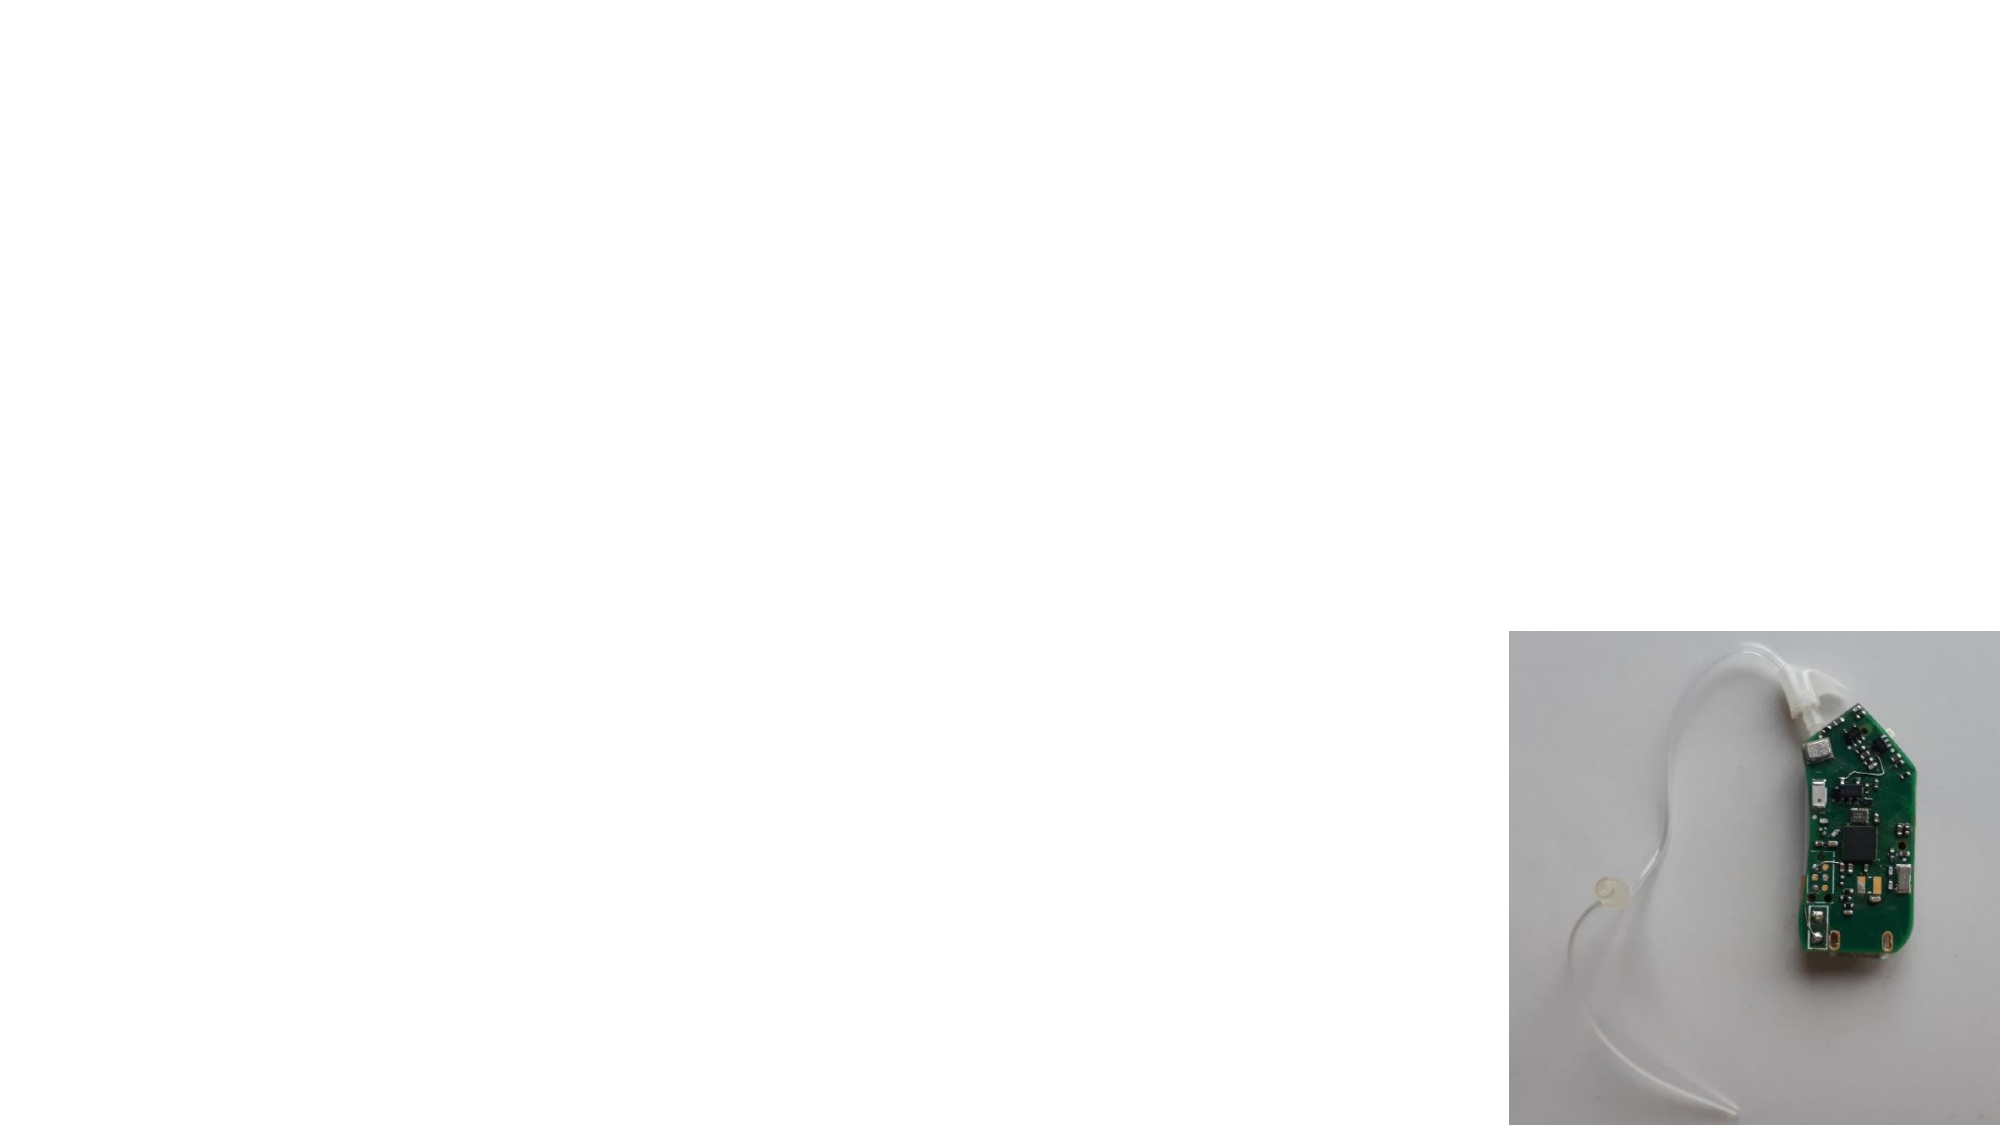
\includegraphics[trim={25.5cm 0cm 0cm 10.7cm},clip,width=\textwidth]{../Chap1/Figure/hearing_aid_Scherer2019.pdf}
					\caption{Appareil auditif \cite{Scherer2019}}
					\label{fig:hearing_aid_Resound}
				\end{subfigure}
				\hfillx
				\begin{subfigure}[t]{0.55\textwidth}
					\captionsetup{justification=centering}
					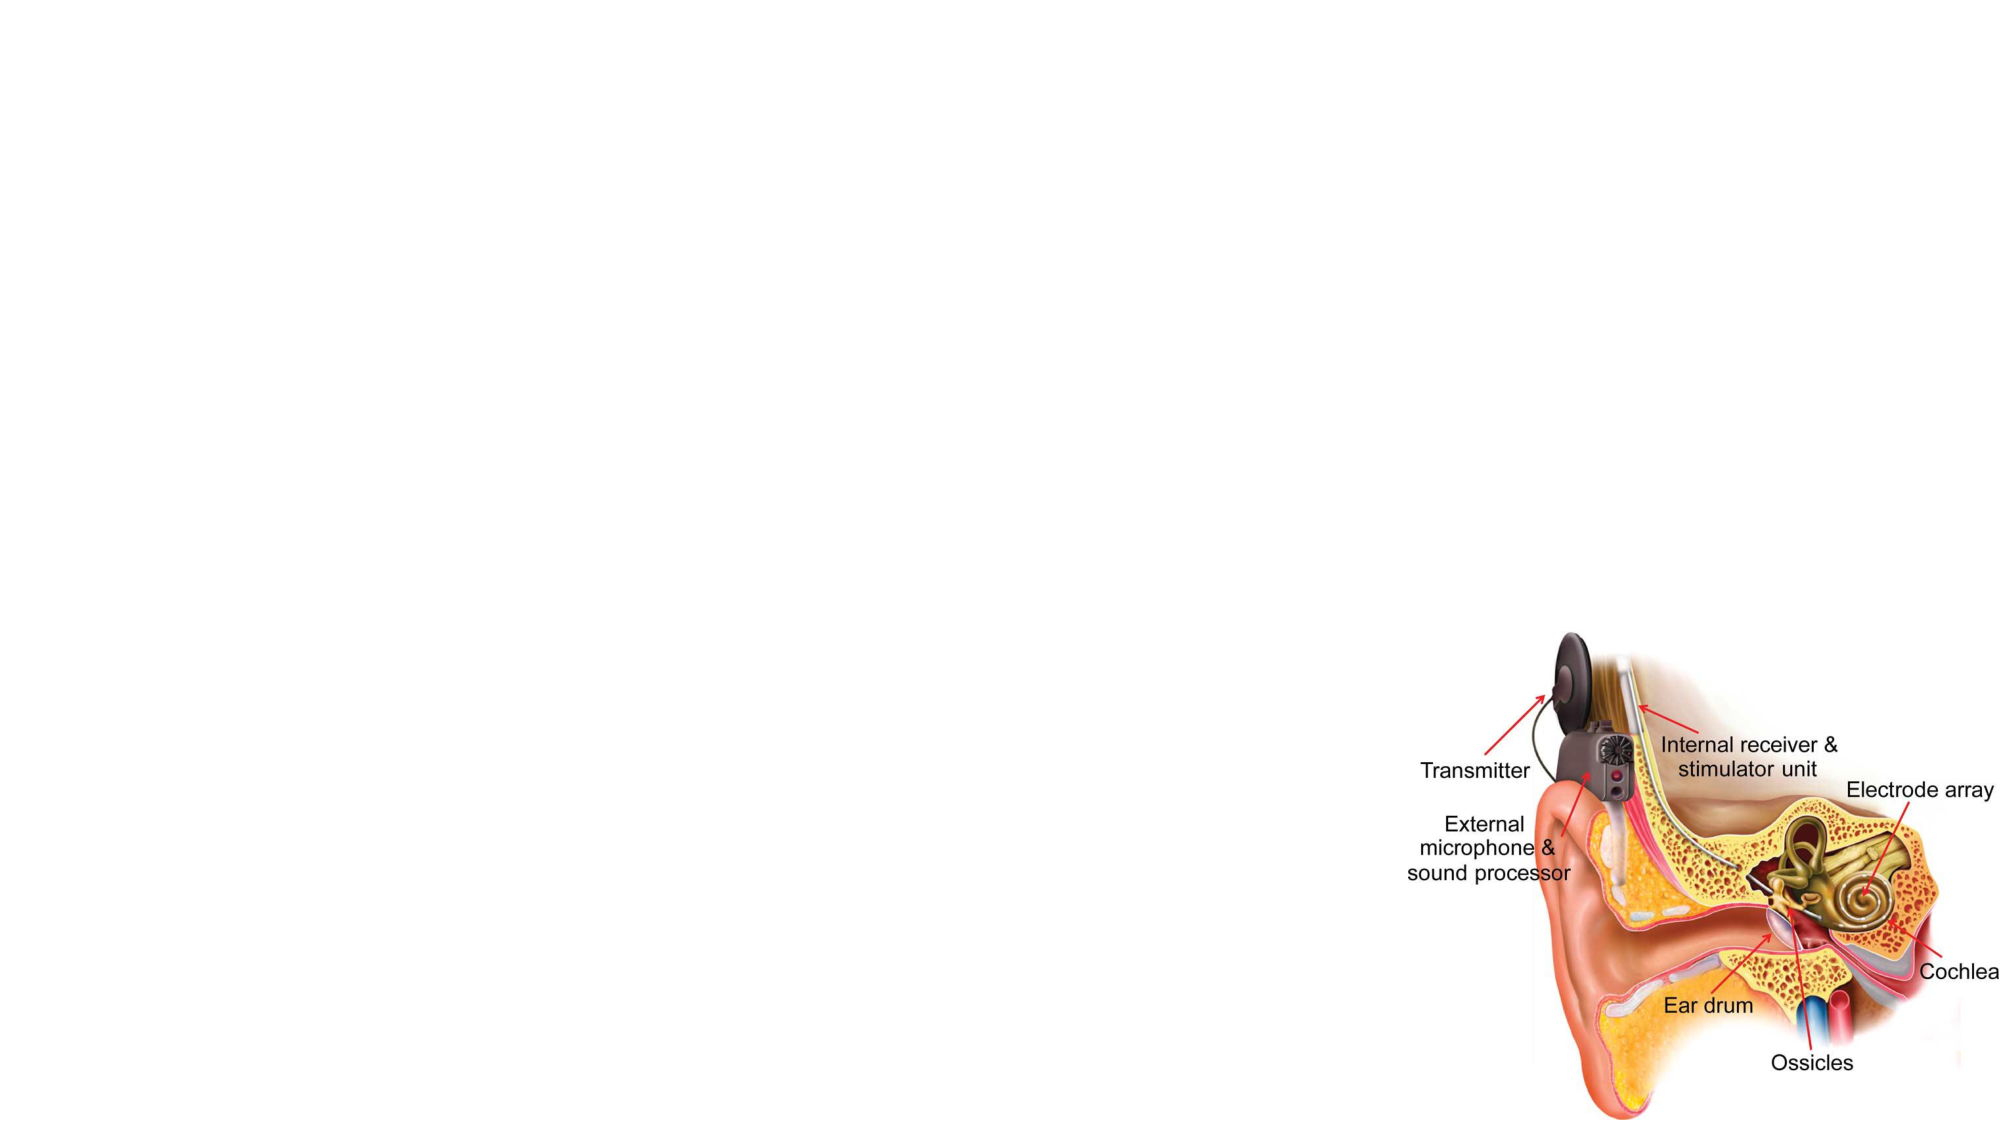
\includegraphics[trim={23.7cm 0cm 0cm 10.5cm},clip,width=\textwidth]{../Chap1/Figure/implant_cochleaire_Yip2015.pdf}
					\caption{Implant cochélaire \cite{Yip2015}}
					\label{fig:implant_Cochlear}
				\end{subfigure}
				\caption{Appareils d'aide à l'audition basse consommation proposés dans la littérature}
				\label{fig:appareils_litterature}
			\end{center}
		\end{figure}
	\end{minipage}
	%%%%%%%%%%%%%%%%
	\hfillx
	\begin{minipage}[c]{0.4\textwidth}
		\resizebox{\textwidth}{!}{%
			\begin{tabular}{ l l l}
				\toprule
				\rowcolor{blue!10}
				\textbf{Réf.}      & \textbf{Puissance} & \textbf{Énergie sur 12h} \\
				\midrule
				\rowcolor{black!8}
				\cite{Scherer2019} & [0.8-1.5]mW        & [35-65]J                 \\
				\cite{Yip2015}     & 0.572mW            & 25J                      \\
				\cite{Kulah2022}     & 0.472mW          & 20J                      \\
				\bottomrule
			\end{tabular}}
		\caption{Consommation énergétique des appareils proposés dans la littérature}
		\label{tab:appareils_litterature_conso}
	\end{minipage}
\end{table}
%%%%%%%%%%%%%%%%
Sur les figures \ref{fig:appareils_litterature} et \ref{fig:cochleaire_MEMS} sont présentés trois dispositifs d'aide à l'audition incluant simplement les fonctions primaires et le tableau \ref{tab:appareils_litterature_conso} donne leurs valeurs de consommations énergétiques.

L'appareil auditif utilise un micro pour capter le son et génère un son amplifié et filtré dans l'oreille. L'implant cochléaire possède aussi un micro extérieur pour capter le son, mais génère des signaux électriques dans la cochlée afin que le cerveau les interprète. La génération de signaux électriques dans la cochlée est un processus moins énergivore que la génération de son filtré et amplifié pour le tympan, c'est pourquoi les implants cochléaires consomment généralement moins. Une solution récente d'implant cochléaire a été proposée en 2022 par Kulah \emph{et al.} \cite{Kulah2022}. Le dispositif est capable de fonctionner à des puissances inférieures à 0.5mW et intègre par ailleurs un récupérateur d'énergie piézoélectrique dont la densité de puissance très importante a été estimée à 1.5mW/cm$^3$ pour une entrée sonore de 120dB. Le récupérateur doit être solidaire du tympan pour exploiter son énergie mécanique de vibration (fig. \ref{fig:cochleaire_MEMS}). Il est composé d'un empilement de transducteurs piézoélectriques \emph{MEMS} multifréquence et collé sur un substrat flexible pour l'interfaçage cutané.
%%%%%%%%%%%%%%%%%%%%%%%%%%%%%%%%%%%%%%
\begin{figure}[!htbp]
	\begin{center}
		\captionsetup{justification=centering}
		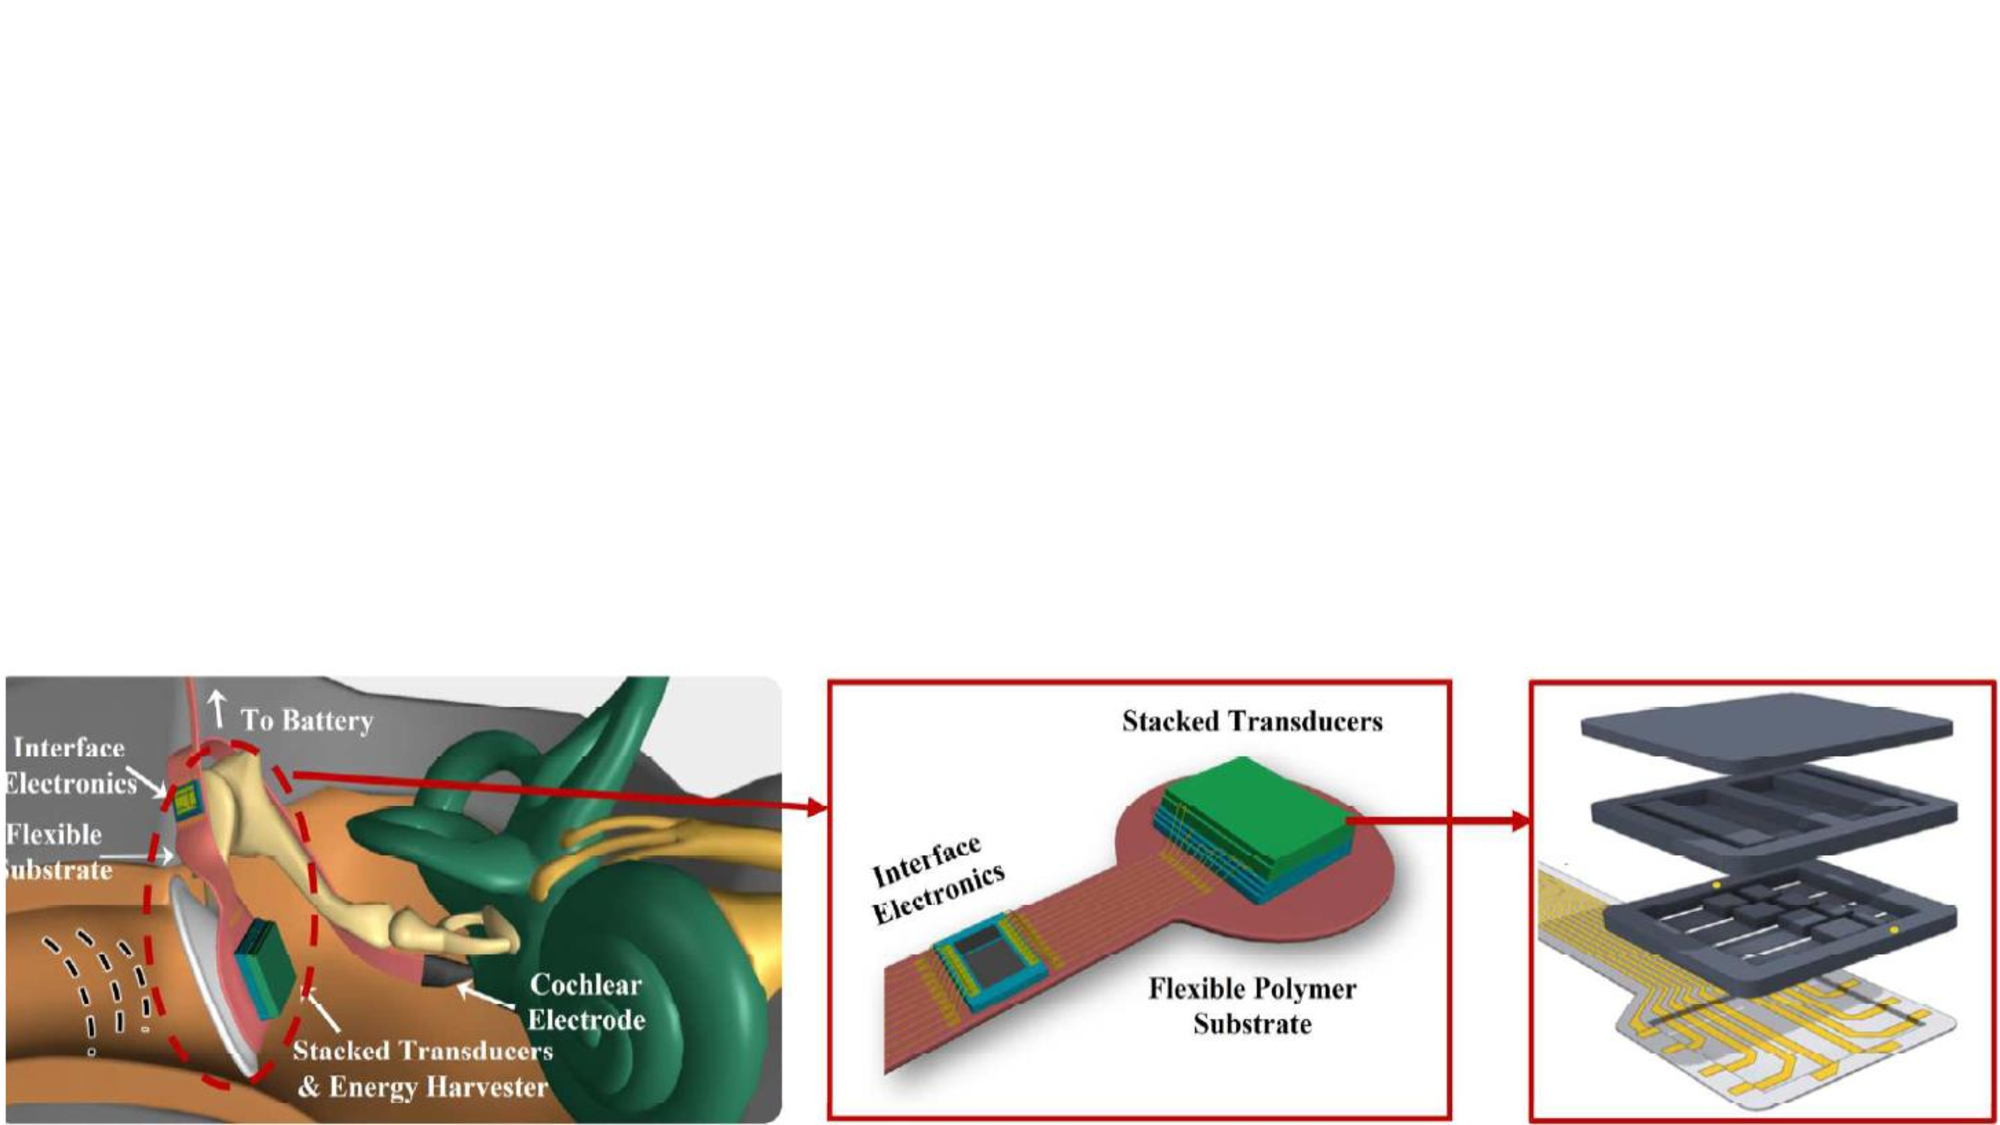
\includegraphics[trim={0cm 0cm 0cm 11.5cm},clip, width=\textwidth]{../Chap1/Figure/cochleaire_MEMS.pdf}
		\caption{Implant cochléaire bio-intégrable proposé par Kulah \emph{et al.} \cite{Kulah2022}.}
		\label{fig:cochleaire_MEMS}
	\end{center}
\end{figure}
%%%%%%%%%%%%%%%%%%%%%%%%%%%%%%%%%%%%%%

Une étude de 2019 montre un aperçu de la durée de cycle des implants cochléaires commerciaux avec les solutions d'alimentations jetables de type pile bouton ou bien avec les batteries rechargeables \cite{ASL-Kids2019}. Elle informe que l'autonomie minimum des dispositifs s'élève à 48 heures avec les solutions jetables et peut descendre à 8-9 heures avec les solutions rechargeables. La longévité des batteries est en moyenne calculée entre 365 et 500 cycles de charge/décharge, ce qui impose un remplacement de cette dernière au minimum une fois environ tous les 1,5 ans. Le vieillissement des batteries induit également des cycles de décharge de plus en plus rapides avec la dégradation de la capacité. Cela peut réduire leur autonomie à moins de 6 heures. Une étude de Woodruff \emph{et al.} parue en 2021 a montré que les patients utilisant des appareils auditifs se retrouvent parfois en difficulté pour changer et choisir les batteries de leurs dispositifs \cite{Woodruff2021}. De plus, une étude de \emph{Audiology Practices} datant de 2016 a montré que la majorité des utilisateurs d'appareils d'aide à l'audition préfère les piles jetables pour la grande autonomie, mais auraient souhaité des solutions rechargeables si l'autonomie des batteries leur permettait une utilisation journalière complète \cite{PracticesAudiology2016}. Ces arguments motivent le développement de systèmes de récupération d'énergie pour complémenter l'apport des batteries afin de prévenir une décharge prématurée des dispositifs. Il est alors intéressant de caractériser les sources d'énergie disponibles autour de l'environnement de l'oreille, et précisément dans le conduit auditif.
    %/////////////////////////////////////////////
	\subsection{Caractérisation de la source d'énergie}
	\label{subsec:1.3.1_Caracterisation la source d energie}
	%////////////////////////////////////////////
La déformation mécanique du CA, découlant des mouvements de la mâchoire, a été étudiée comme source d'énergie par les chercheurs du laboratoire CRITIAS. Carioli \emph{et al.} ont étudié  l'évolution du volume du CA en moulant deux bouchons d'oreille intra-auriculaires sur mesure \cite{Carioli2016}. Le premier a été moulé avec la mâchoire ouverte et l'autre avec la mâchoire fermée. En faisant un balayage spatial sur les géométries résultantes, ils ont pu extraire un modèle numérique 3D (fig. \ref{fig:earcanal_3D}). Ils ont alors constaté que le CA subit une flexion globale sur toute sa longueur, couplée à une compression locale, en fonction de la position de la mâchoire. Ces deux phénomènes découlent de la déformation induite par le joint temporo-mandibulaire (JTM) sur le CA. La figure \ref{fig:schema_JTM} montre une vue schématisée de la déformation mécanique du conduit auditif sous l'action du JTM.
%%%%%%%%%%%%%%%%%%%%%%%%%
\begin{figure}[!htbp]
\begin{center}
	\begin{subfigure}[b]{0.4\textwidth}
    	\captionsetup{justification=centering}
		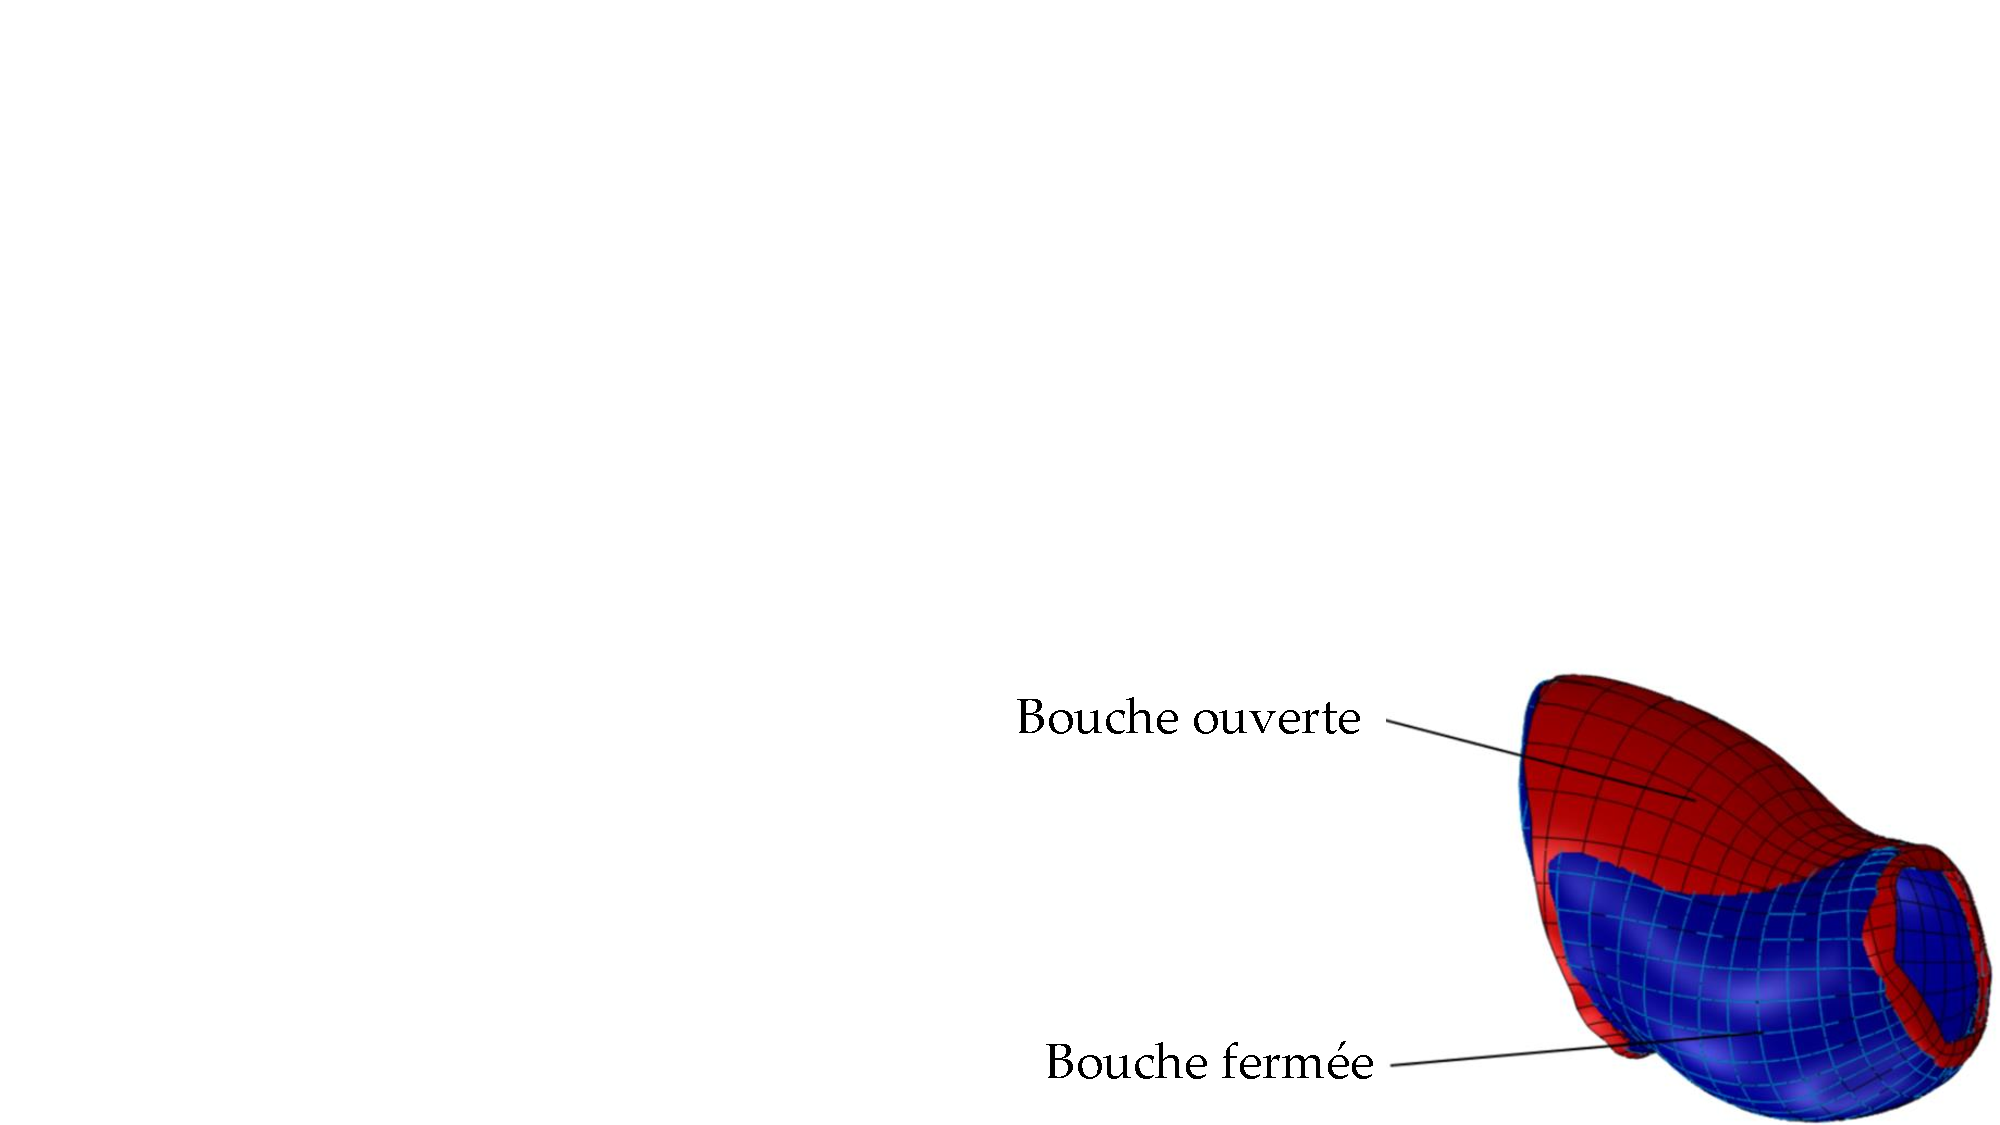
\includegraphics[trim={17cm 0cm 0cm 11cm},clip,width=\textwidth]{../Chap2/Figure/earcanal_3D_a.pdf}
		\caption{}
		\label{fig:earcanal_3D_a}
	\end{subfigure}
\hfillx
	\begin{subfigure}[b]{0.4\textwidth}
    	\captionsetup{justification=centering}
		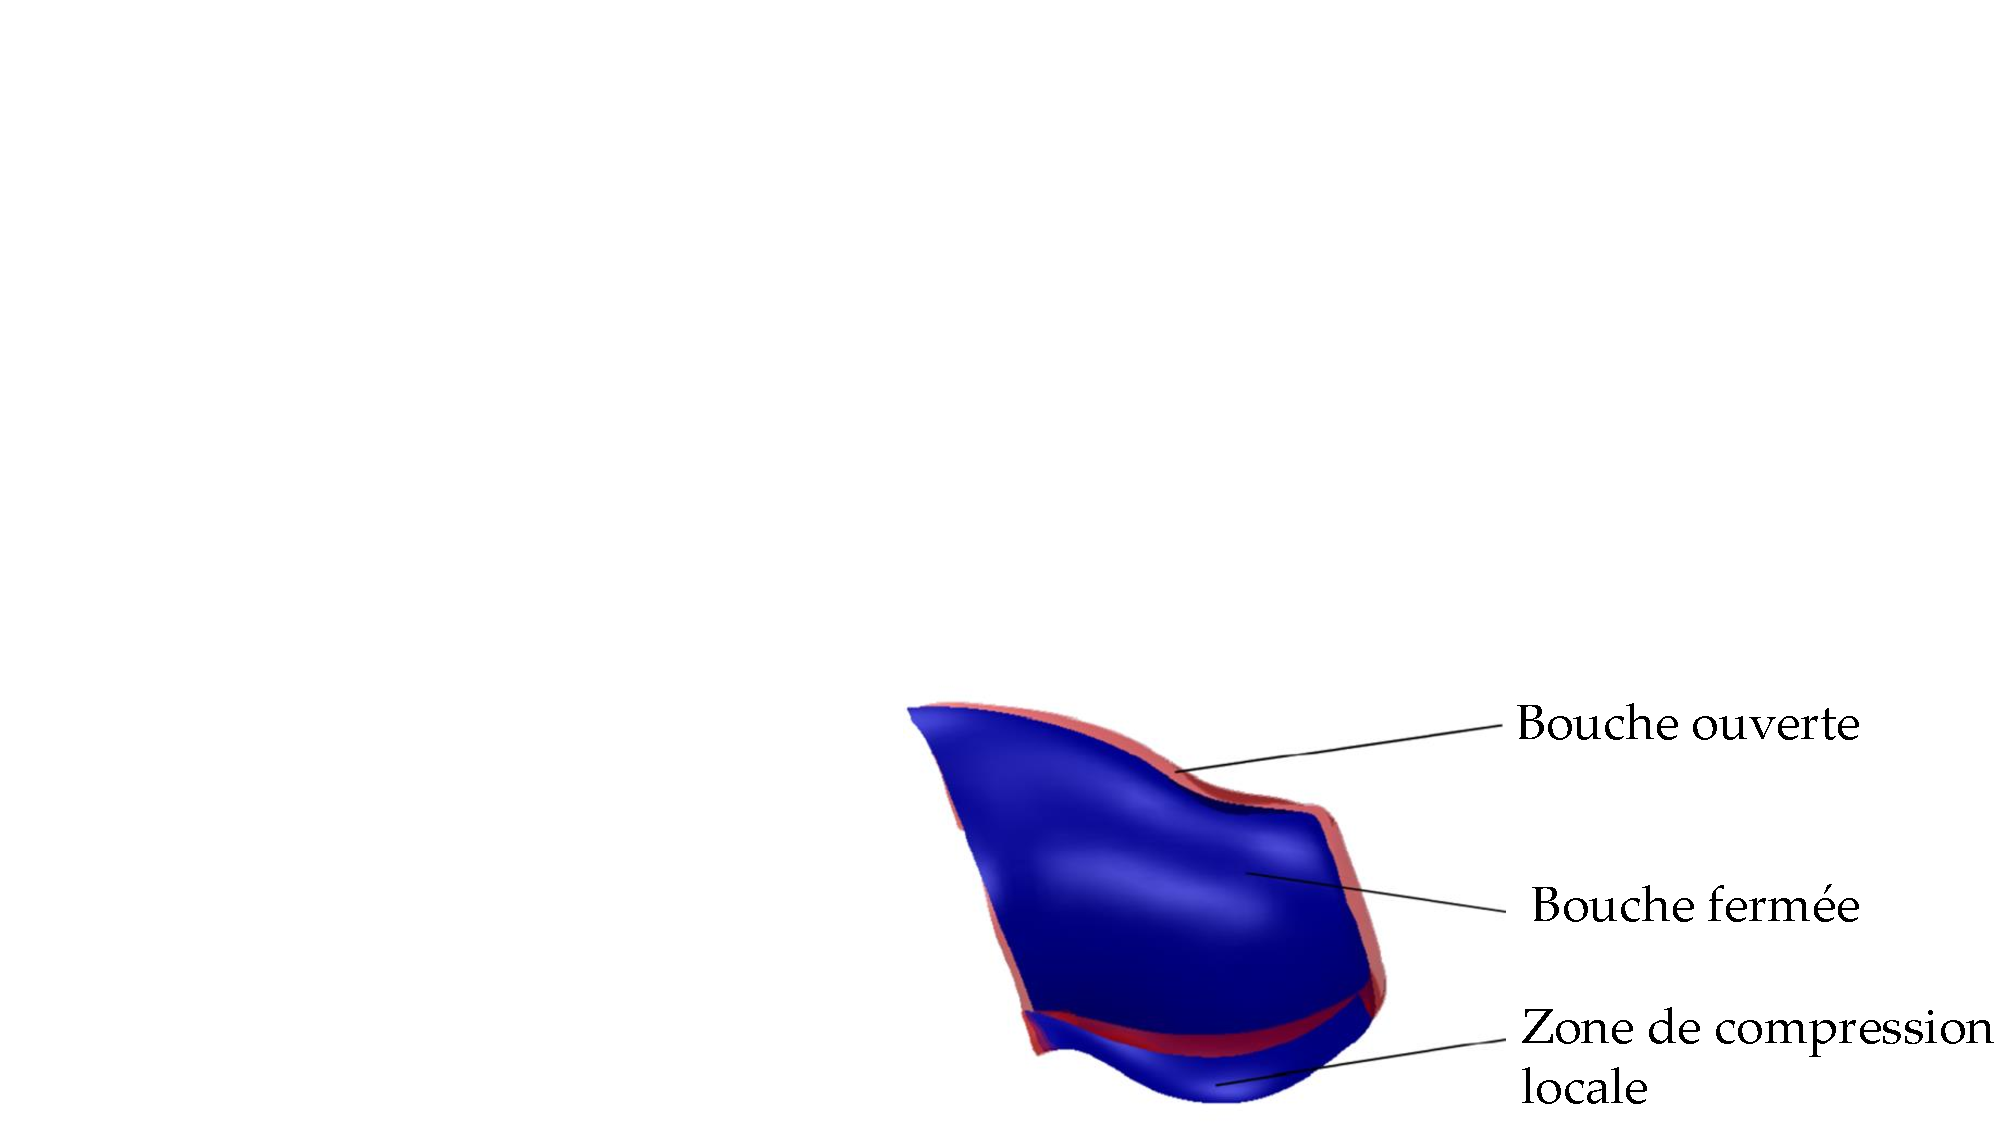
\includegraphics[trim={15cm 0cm 0cm 11cm},clip,width=\textwidth]{../Chap2/Figure/earcanal_3D_b.pdf}
		\caption{}
		\label{fig:earcanal_3D_b}  
	\end{subfigure}
	\caption{(a) CA aux deux positions extrêmes, montrant un mouvement de flexion global. (b) Vue de coupe du CA aux deux positions extrêmes, mettant en évidence une zone de compression locale \cite{Carioli2016}.}
	\label{fig:earcanal_3D}
\end{center}	
\end{figure} 
%%%%%%%%%%%%%%%%
%%%%%%%%%%%%%%%%%%%%%%%%%%%%%%%%%%%%%%
\begin{figure}[!htbp]
	\begin{center}
		\captionsetup{justification=centering}
		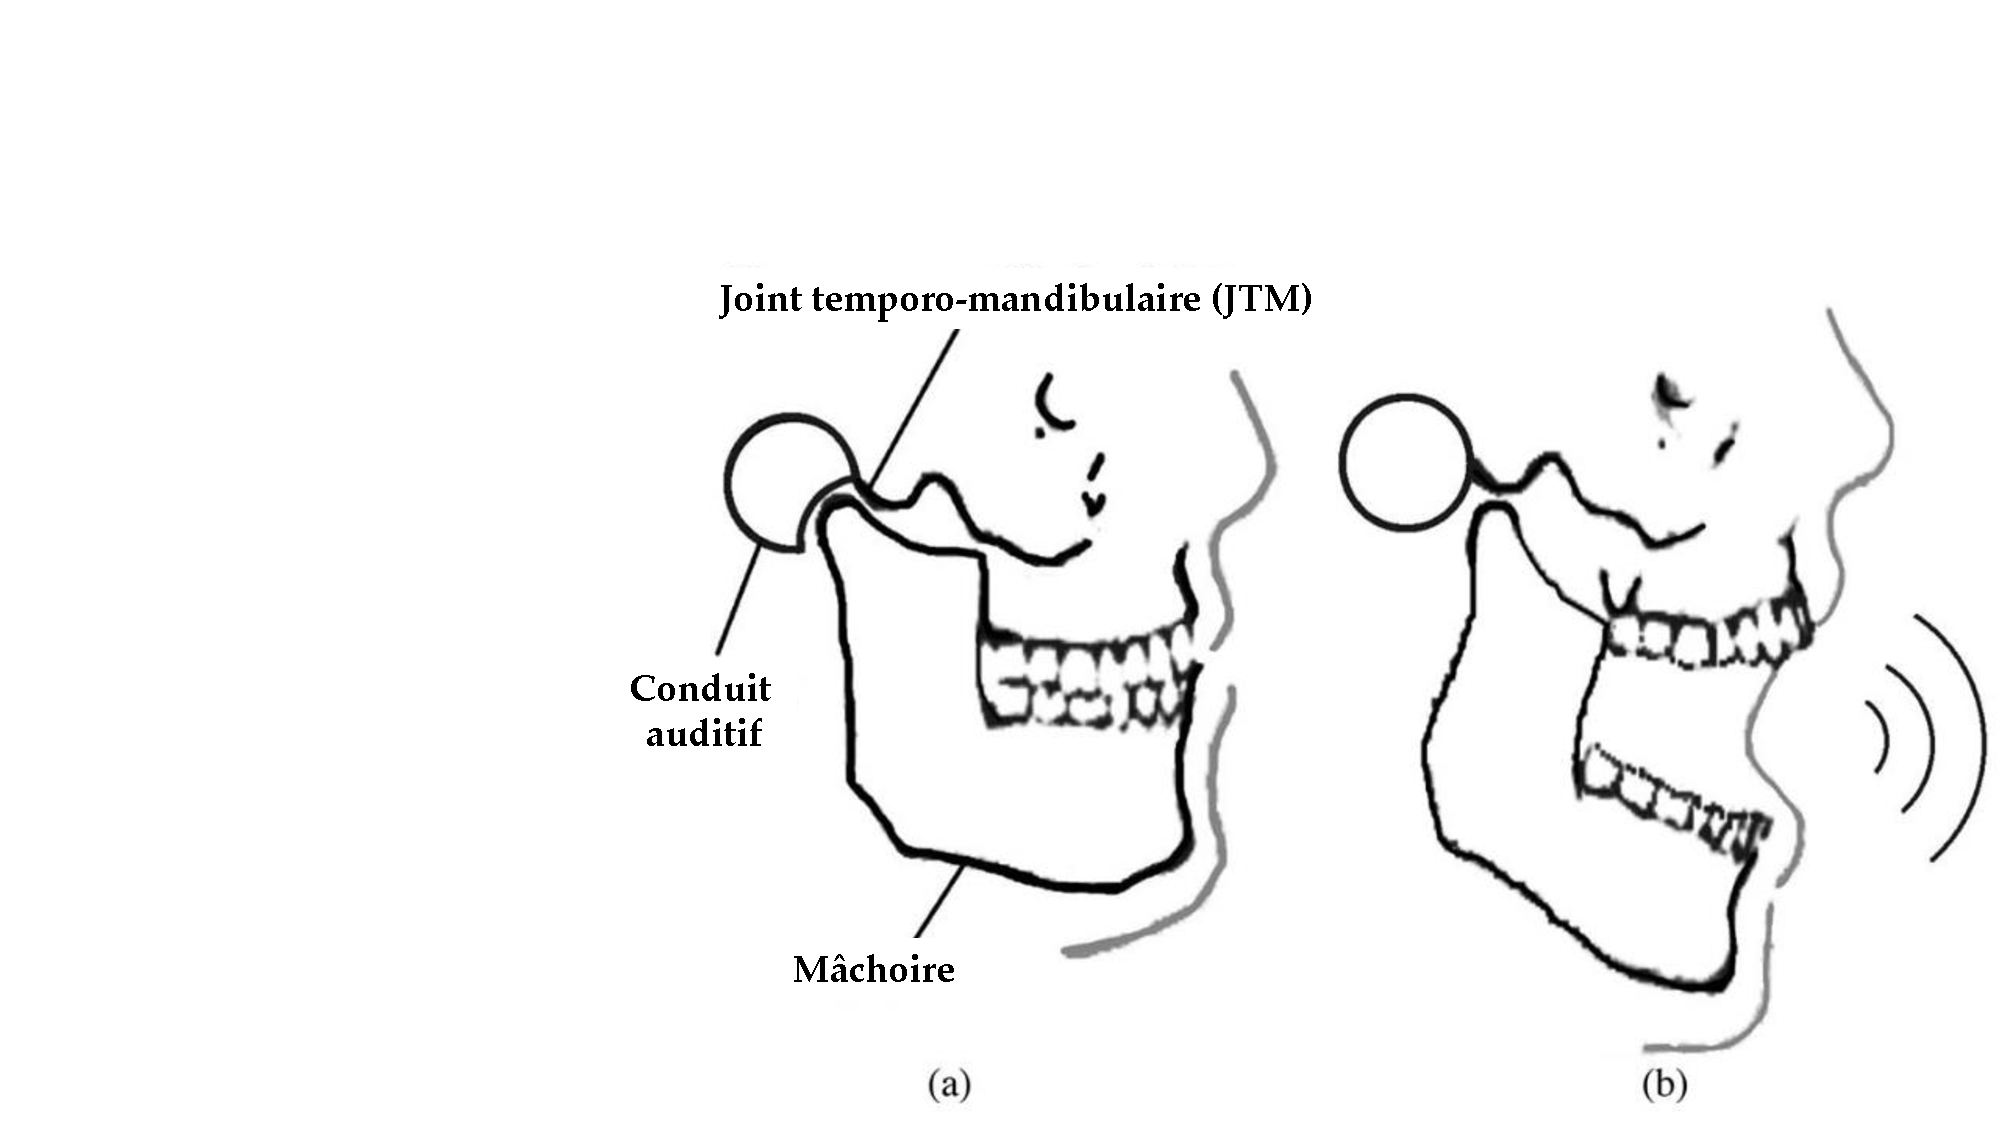
\includegraphics[trim={10.5cm 0cm 0cm 4cm},clip, width=0.6\textwidth]{../Chap1/Figure/schema_JTM.pdf}
		\caption{Schéma de la déformation mécanique du conduit auditif par le JTM \cite{Delnavaz2014}. (a) Bouche fermée. (b) Bouche ouverte.}
		\label{fig:schema_JTM}
	\end{center}
\end{figure}
%%%%%%%%%%%%%%%%%%%%%%%%%%%%%%%%%%%%%%
%\begin{equation}
%	E_{compression} = \int_{0}^{L}\ \dfrac{\pi G (d_{ouvert}(s) - d_{\text{\textit{fermé}}}(s))^2}{4}\ ds
%	\label{eq:energie_compression_earplug}
%\end{equation}
%
%\begin{equation}
%	E_{flexion} = \dfrac{\pi E L}{128}\ \sum\limits_{i=0}^N d^4_{ouvert}(i)\biggl(\kappa_{ouvert}-\kappa_{\text{\textit{fermé}}}\biggr)^2
%	\label{eq:energie_flexion_earplug}
%\end{equation}

À partir du modèle numérique de la variation de volume du CA et des \mbox{caractéristiques} du silicone composant les bouchons d'oreille, ils ont pu estimer l'énergie nécessaire à générer ces déformations. Une étude a été menée sur 12 sujets et les résultats pour chaque individu sont présentés dans le tableau \ref{tab:earcanal_energie_estimation_subjects}.
%%%%%%%%%%%%%%%%%%%%%%%%%%%%%%%%%%%%%%%%%%%
\begin{table}[!htb]
\centering
\begin{tabular}{c}
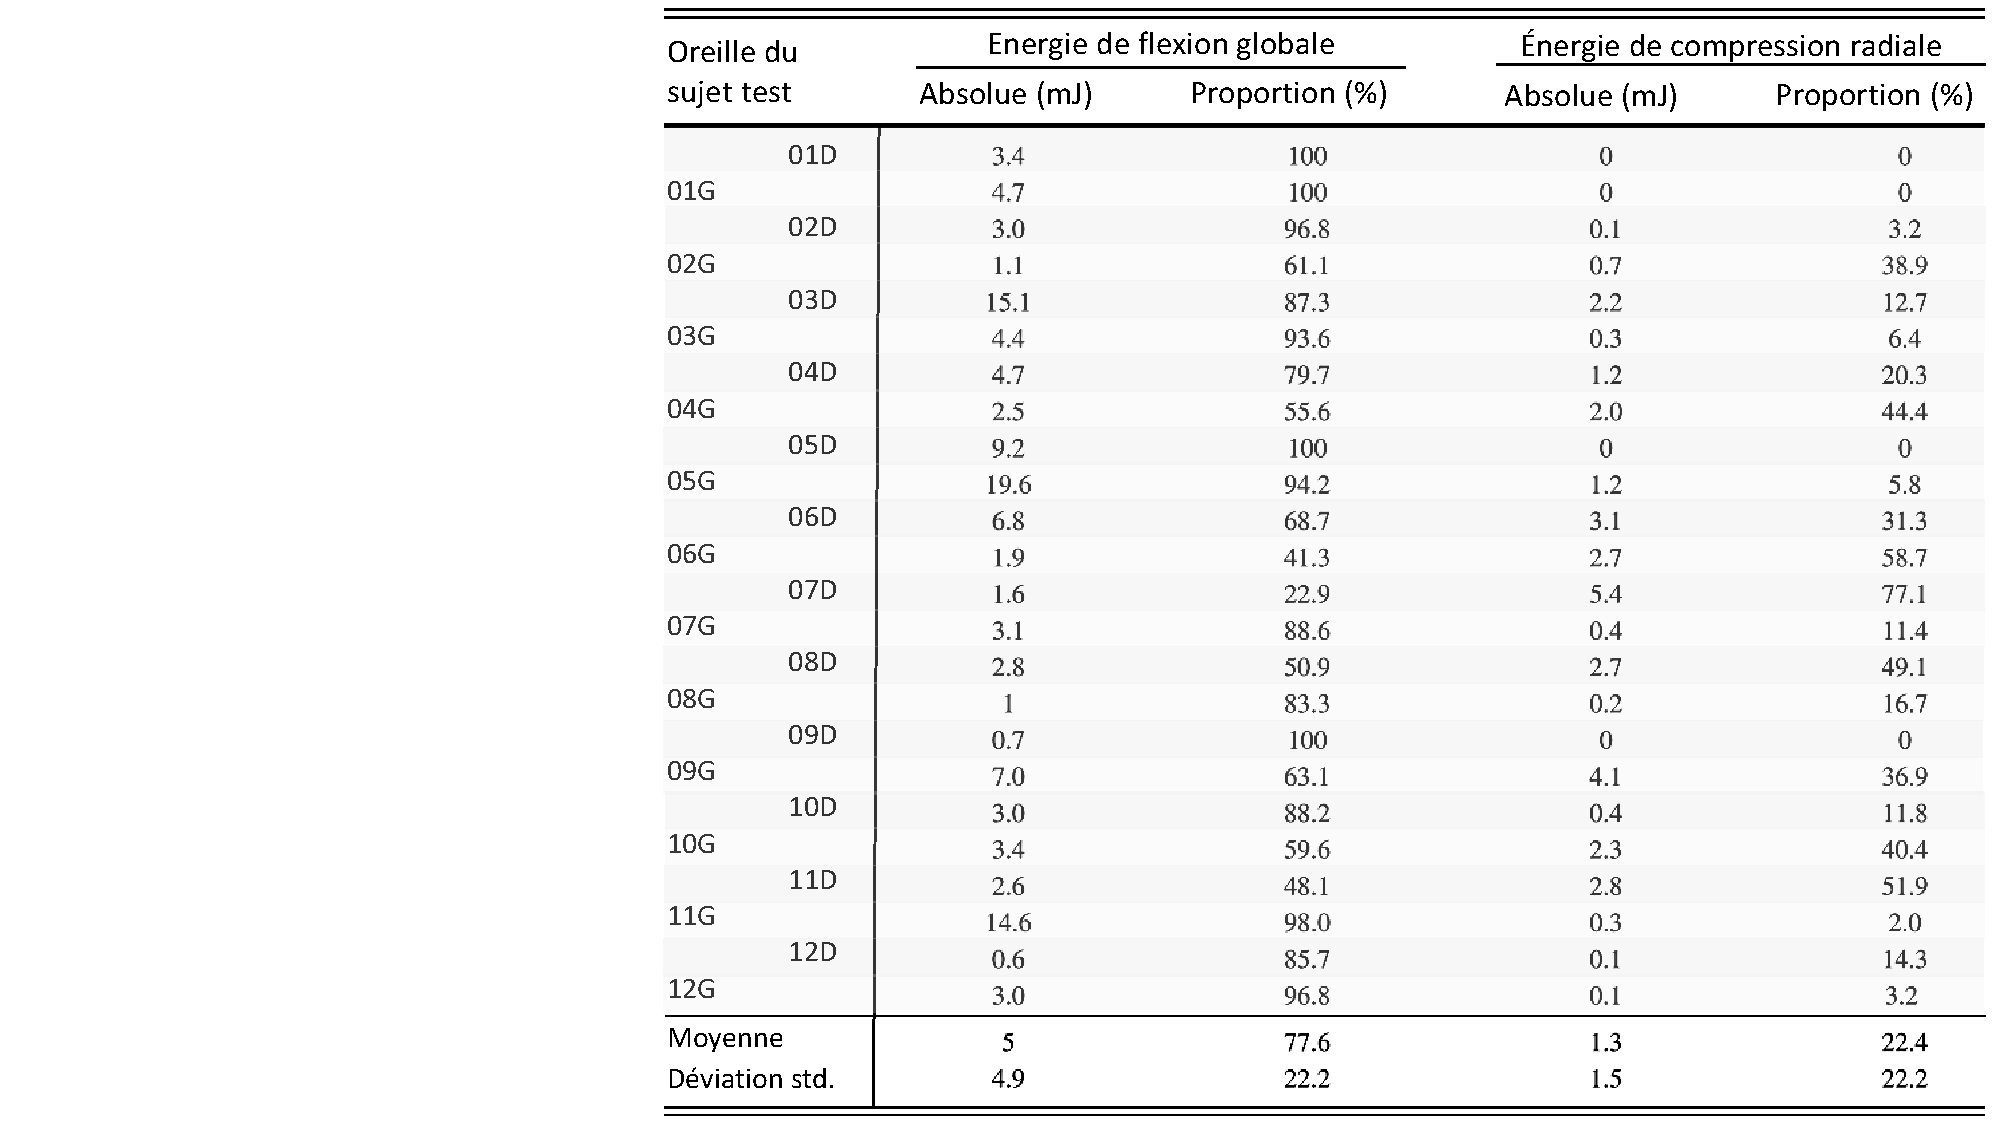
\includegraphics[trim={11cm 0cm 0cm 0cm},clip, width=0.8\textwidth]{../Chap2/Figure/earcanal_energie_estimation_subjects.pdf}
\end{tabular}
\caption{Énergie de flexion globale, de compression radiale et leurs proportions pour l'oreille gauche(G) et droite(D) pour 3 sujets femelle et 9 sujets mâle, âgés de 24 à 60 ans \cite{Carioli2016}.}
\label{tab:earcanal_energie_estimation_subjects}
\end{table} 
%%%%%%%%%%%%%%%%%%%%%%%%%%%%%%%%%%%%%%%%%%%

On relève une disparité notable entre les individus et même entre les deux oreilles d'un seul et même individu. L'énergie de compression est de surcroît absente chez certaines personnes. En faisant la moyenne sur les 24 oreilles testées, on s'aperçoit que le gisement d'énergie de flexion est 5 fois supérieur à celui de compression. Néanmoins, l'énergie récupérable grâce à l'un ou l'autre type de contrainte sera fortement dépendant de l'efficacité de conversion énergétique des dispositifs respectivement adaptés à chacun des deux types de sources. En effet, les tissus mous et le faible volume offert par le CA rendent complexe l'intégration in situ de la majorité des technologies conventionnelles de récupération d'énergie.

L'étude précédente prend seulement en compte la différence de volume du bouchon d'oreille moulé sur mesure dans les positions extrêmes de la mâchoire. En ce sens, il est supposé que le travail de la force générée par la pression du JTM sur le CA est capable de déformer le bouchon d'oreille depuis une position extrême à l'autre. En d'autres termes, l'oreille est considérée comme ayant une impédance mécanique infinie, ce que nous savons être inexact, car elle est composée de tissus mous du corps humain.
%%%%%%%%%%%%%%%%%%%%%%%%%
\begin{figure}[!htbp]
\begin{center}
	\begin{subfigure}[t]{0.66\textwidth}
    	\captionsetup{justification=centering}
		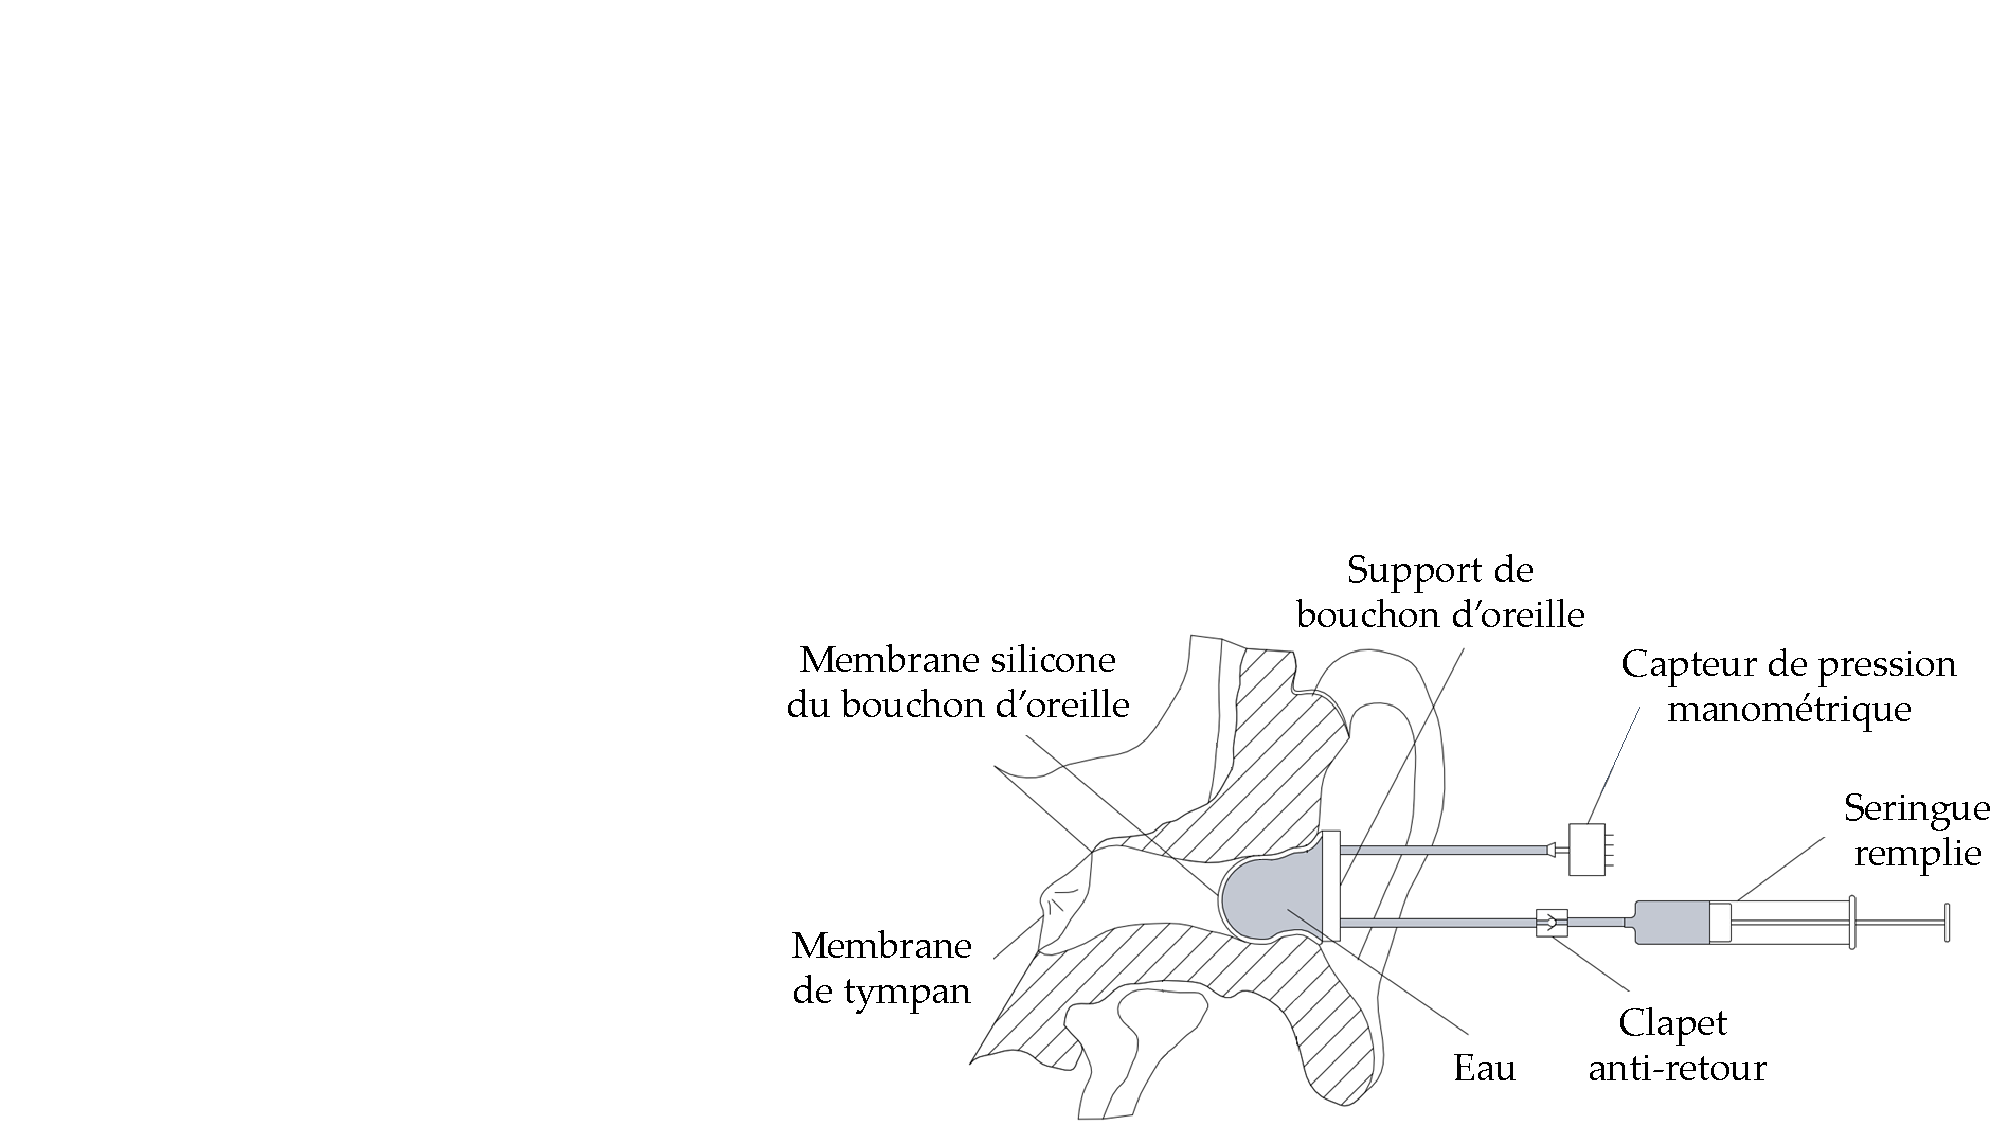
\includegraphics[trim={13.2cm 0cm 0cm 9.4cm},clip,width=\textwidth]{../Chap2/Figure/Bouchard_BDT.pdf}
		\caption{Remplissage du bouchon d'oreille}
		\label{fig:Bouchard_BDT}
	\end{subfigure}
\hfillx
	\begin{subfigure}[t]{0.28\textwidth}
    	\captionsetup{justification=centering}
		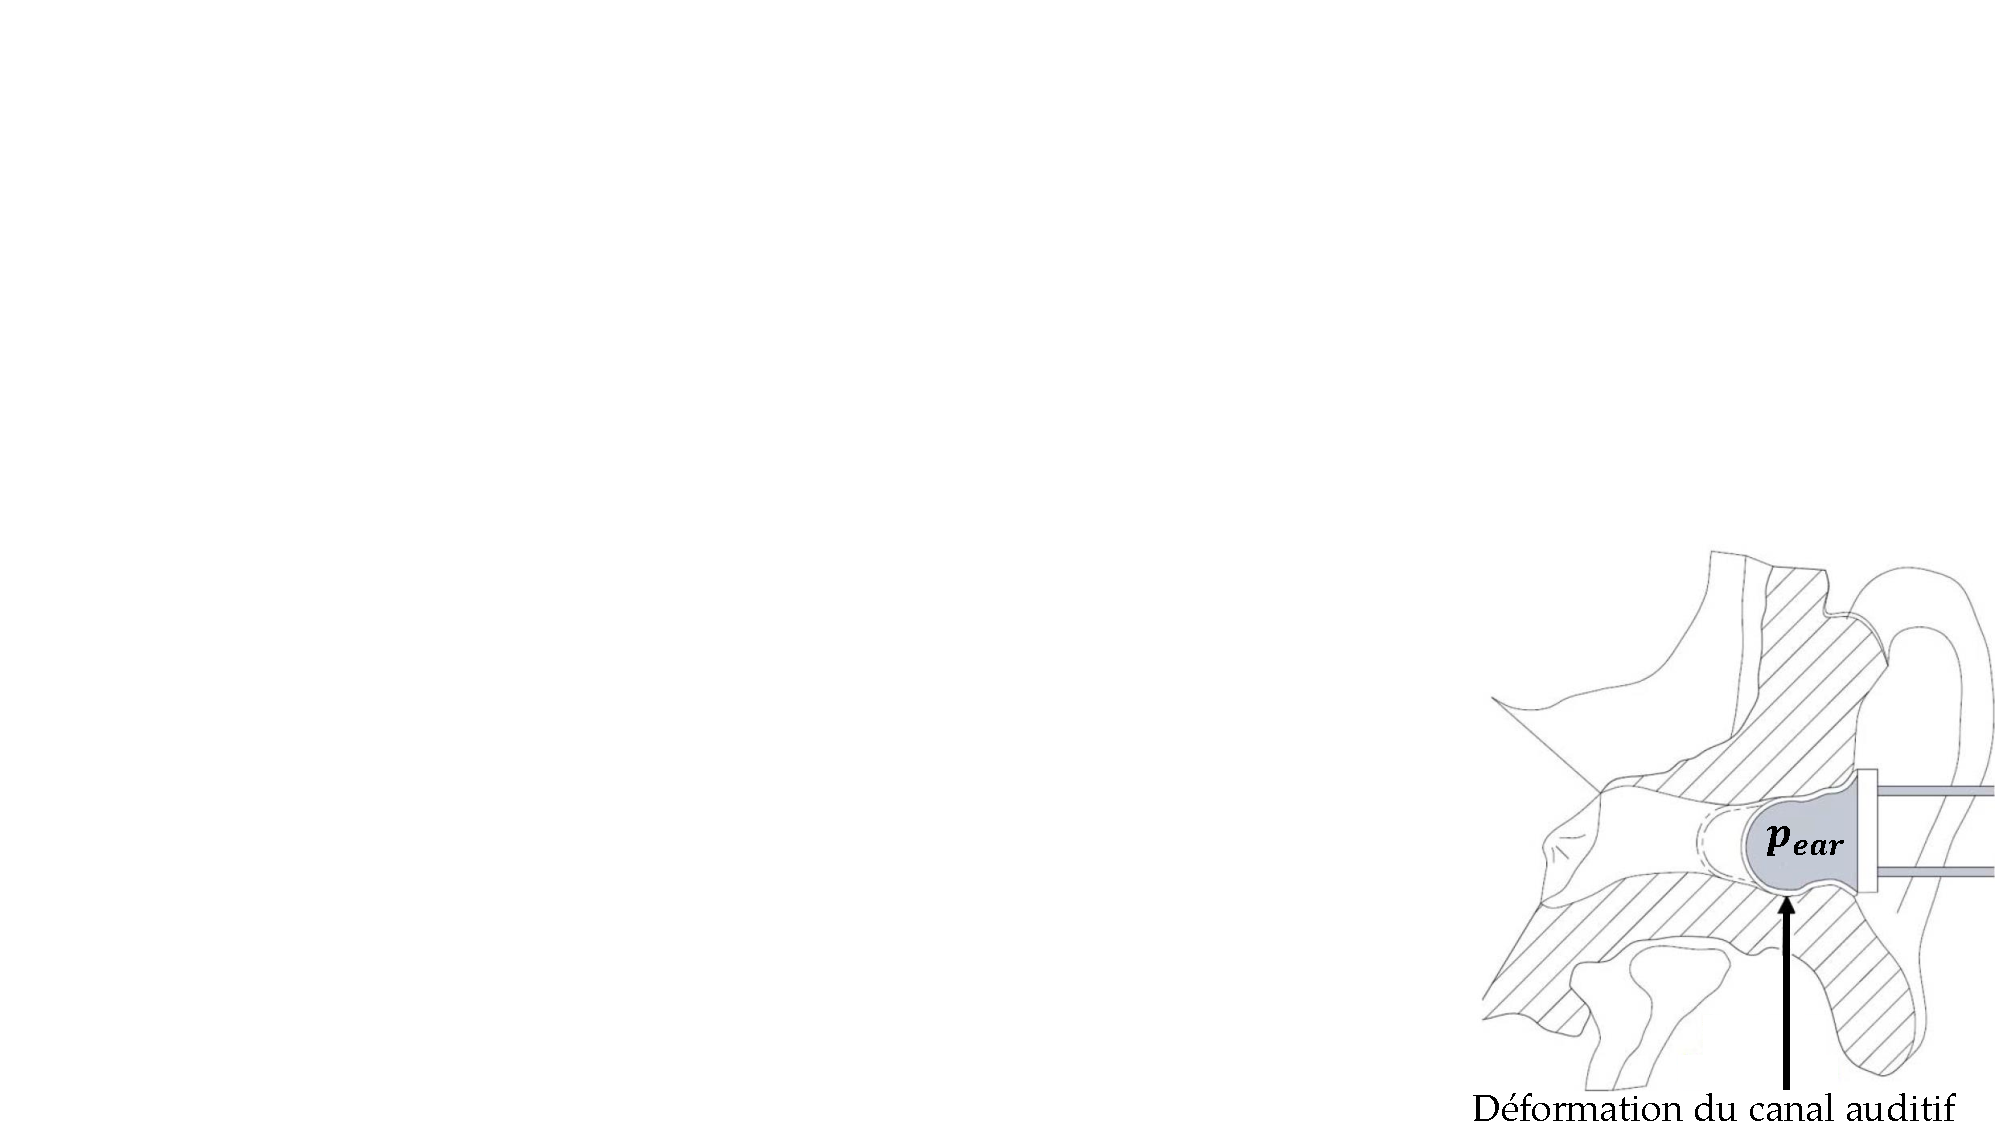
\includegraphics[trim={24.8cm 0cm 0cm 9cm},clip,width=\textwidth]{../Chap2/Figure/Bouchard_essais.pdf}
		\caption{Déformation du bouchon d'oreille durant la mastication}
		\label{fig:Bouchard_essais}  
	\end{subfigure}
	\caption{Essais de caractérisation du gisement énergétique de compression dans le CA \cite{Bouchard-Roy2020}.}
	\label{fig:Bouchard-Roy2020_gisement_compression}
\end{center}	
\end{figure} 
%%%%%%%%%%%%%%%%	

À cet effet, d'autres travaux ont suivi pour une meilleure caractérisation du gisement énergétique, en prenant cette fois-ci en compte l'impédance mécanique de la paroi du CA. L'énergie de compression a par exemple été davantage caractérisée par Bouchard \emph{et al.} par essais expérimentaux sur 6 sujets âgés de 20 à 35 ans \cite{Bouchard-Roy2020}. Pour ce faire, un bouchon d'oreille en silicone a été pressurisé à l'eau à une pression $p_{ear} = p_{gon}$, de façon à ce qu'il épouse correctement la paroi du CA. Un schéma du protocole de remplissage est présenté sur la figure \ref{fig:Bouchard_BDT}. La pression minimale nécessaire pour assurer le bon contact oreille/bouchon, a été évaluée à 14kPa d'après le brevet déposé sur le dispositif de remplissage \cite{TURCOT2011}. Le protocole d'essais consistait alors à mesurer l'évolution de la pression $p_{ear}$ durant la mastication avec le bouchon pressurisé. Les composants du circuit hydraulique ont été considérés infiniment rigides devant le bouchon d'oreille. Les essais ont été réalisés en circuit hydraulique ouvert, de sorte que la résistance rencontrée par l'oreille soit la seule rigidité du bouchon d'oreille qui se voit alors déformé selon le dessin de la figure \ref{fig:Bouchard_essais}. Les résultats de variation de $p_{ear}$ durant un repas, pour le sujet 1, sont alors présentés sur la figure \ref{fig:Bouchard_pression_puissance}.
%%%%%%%%%%%%%%%%%%%%%%%%%%%%%%%%%%%%%%
\begin{figure}[!htbp]
\begin{center}
    \captionsetup{justification=centering}
	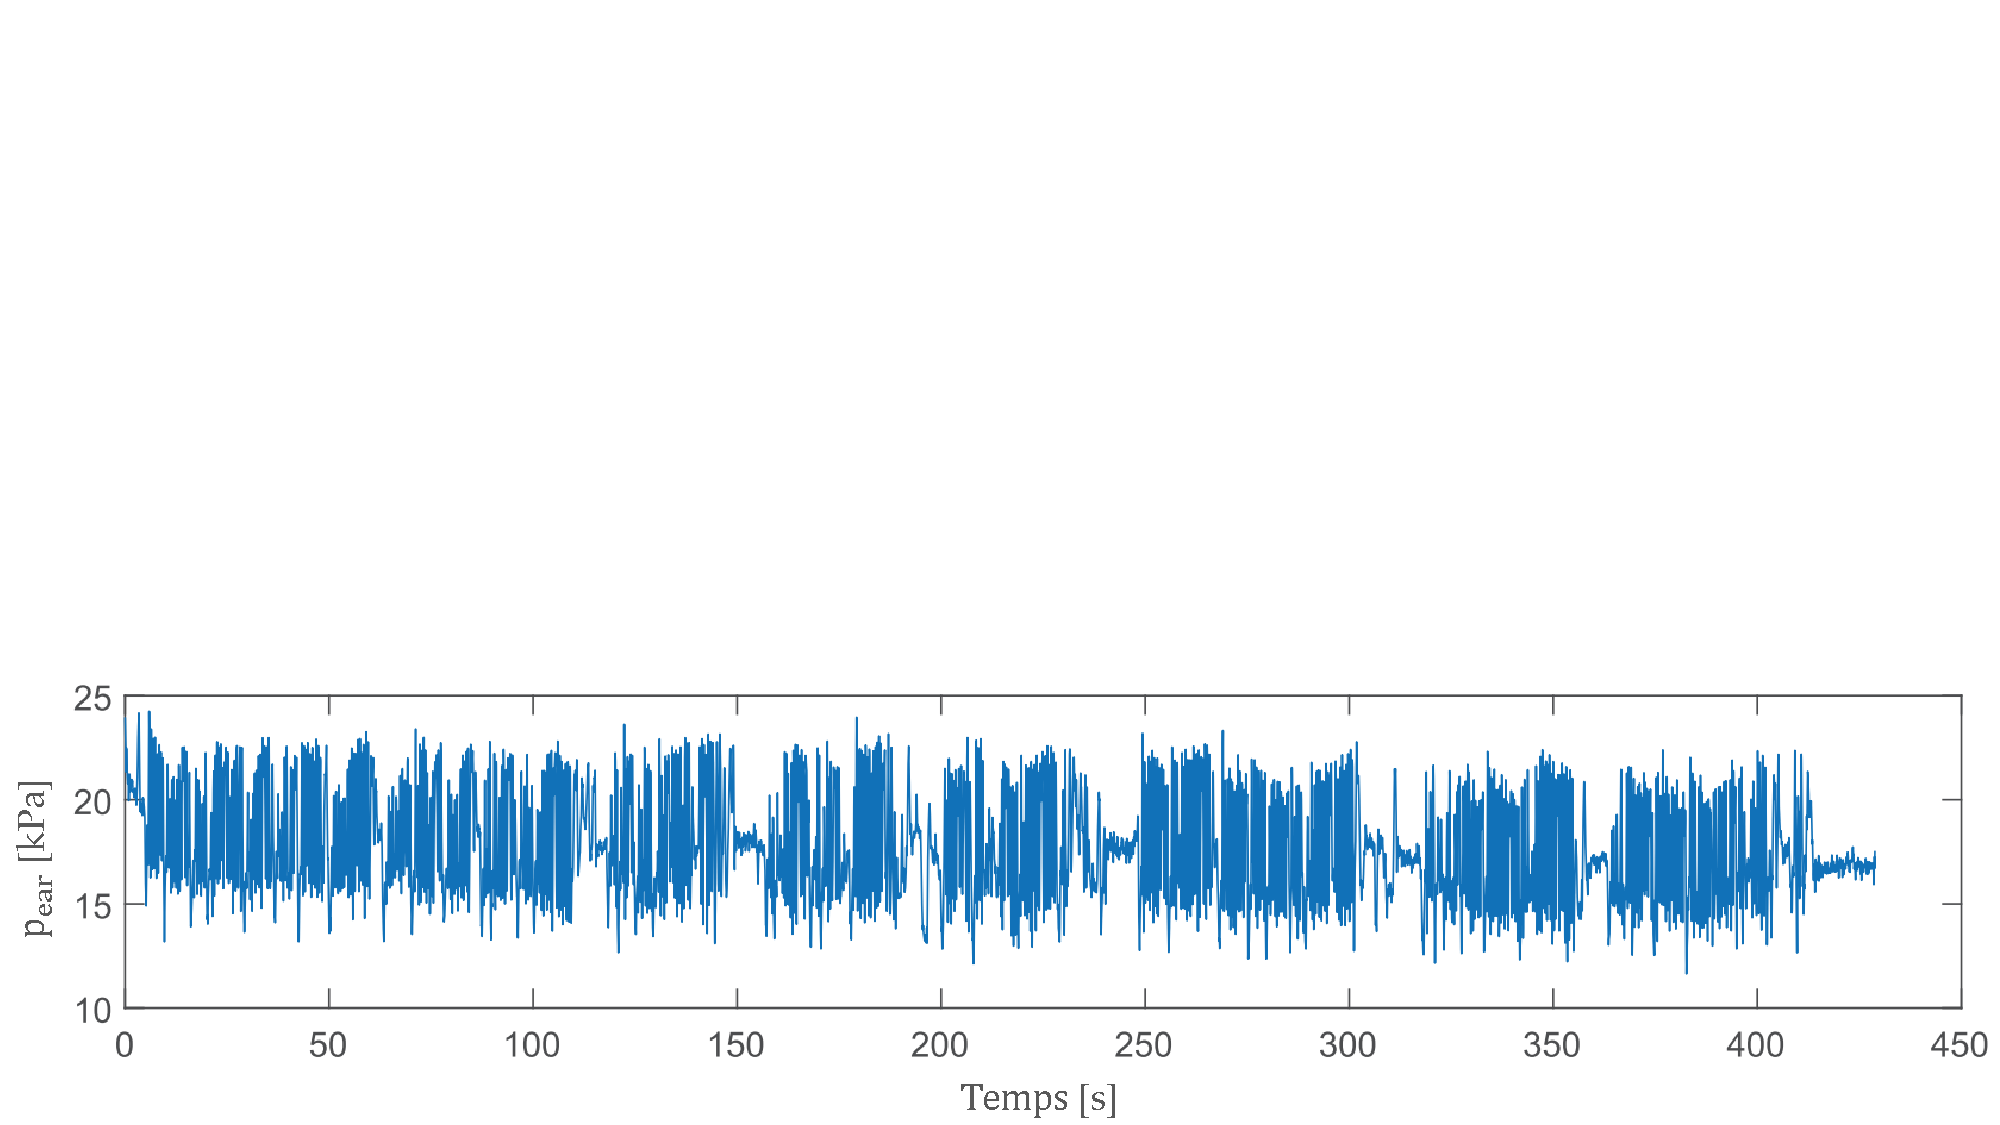
\includegraphics[trim={0cm 0cm 0cm 11cm},clip, width=\textwidth]{../Chap2/Figure/Bouchard_pression.pdf}
	\caption{Résultats de la variation de pression dans le bouchon d'oreille durant un repas pour le sujet \ang{n}1 \cite{Bouchard-Roy2020}.}
	\label{fig:Bouchard_pression_puissance}
\end{center}
\end{figure}
%%%%%%%%%%%%%%%%%%%%%%%%%%%%%%%%%%%%%%

La pression générant le travail de déformation mécanique sur le bouchon d'oreille est la variation $\Delta p_{ear}$ qui se produit durant les mouvements de la mâchoire. Celle-ci est fonction de la pression $p_{gon}$ initiale. Le tableau \ref{tab:Bouchard_deltaPmax} présente alors les résultats de la variation $\Delta p_{ear}$ observée sur un sujet en fonction du niveau de pressurisation initial du bouchon d'oreille. Ce jeu de données expérimentales ne prend pas en compte le volume de déformation, mais donne un ordre de grandeur des pressions atteignables en fonction du remplissage initial.
%%%%%%%%%%%%%%%%%
\begin{table}[!htbp]
	\centering
	\captionsetup{justification=centering}
	\rowcolors[]{2}{black!8}{}{
	\begin{tabular}{| c || c|c|c|c|c|c|}
\hline		 
\cellcolor{blue!10}{{\textbf{$p_{gon}~[kPa]$}}}
 &15.0 & 17.0 & 19.0 & 21.0 & 23.0 & 27.0 \\	\hline 
\cellcolor{blue!10}{{\textbf{$\Delta p_{ear}~[kPa]$}}}
 & 3.30 & 4.23 & 5.17 & 6.50 & 7.72 & 12.31 \\	\hline 
		\end{tabular}}
        \caption{Variations de pression $\Delta p_{ear}$ maximales en fonction de la \mbox{pressurisation initiale $p_{gon}$}}
        \label{tab:Bouchard_deltaPmax}
\end{table} 
%%%%%%%%%%%%%%%%%%%%%

Nous allons voir dans la suite trois exemples de dispositifs, visant à récupérer l'énergie de flexion et/ou de compression du JTM sur le CA. Nous allons alors tenter de mettre en évidence les défis rencontrés pour la récupération de l'énergie de déformation du CA. Aussi nous proposerons une nouvelle architecture de dispositif qui vise à répondre aux défis posés en maximisant le rendement de conversion d'énergie.
    %/////////////////////////////////////////////
	\subsection{État de l'art sur les récupérateurs existants}
	\label{subsec:1.4.3_Etat de l art sur les recuperateurs existants}
	%////////////////////////////////////////////
L'énergie exploitable dans l'oreille doit nécessairement être captée au travers d'une interface mécanique, les parois d'un bouchon d'oreille dans notre cas. La question se pose ensuite de convertir cette énergie mécanique en électrique en minimisant les pertes. La littérature propose à ce jour 2 stratégies principales pour la récupération d'énergie issue de la déformation du CA. La première est d'utiliser un polymère piézoélectrique enroulé autour d'un bouchon d'oreille moulé sur mesure \cite{Delnavaz2013}. La figure \ref{fig:conversion_critias_pvdf} illustre la chaîne de conversion énergétique depuis l'oreille jusqu'à l'unité de stockage pour cette solution.
%%%%%%%%%%%%%%%%%%%%%%%%%%%%%%%%%%%%%%
\begin{figure}[!htbp]
\begin{center}
    \captionsetup{justification=centering}
	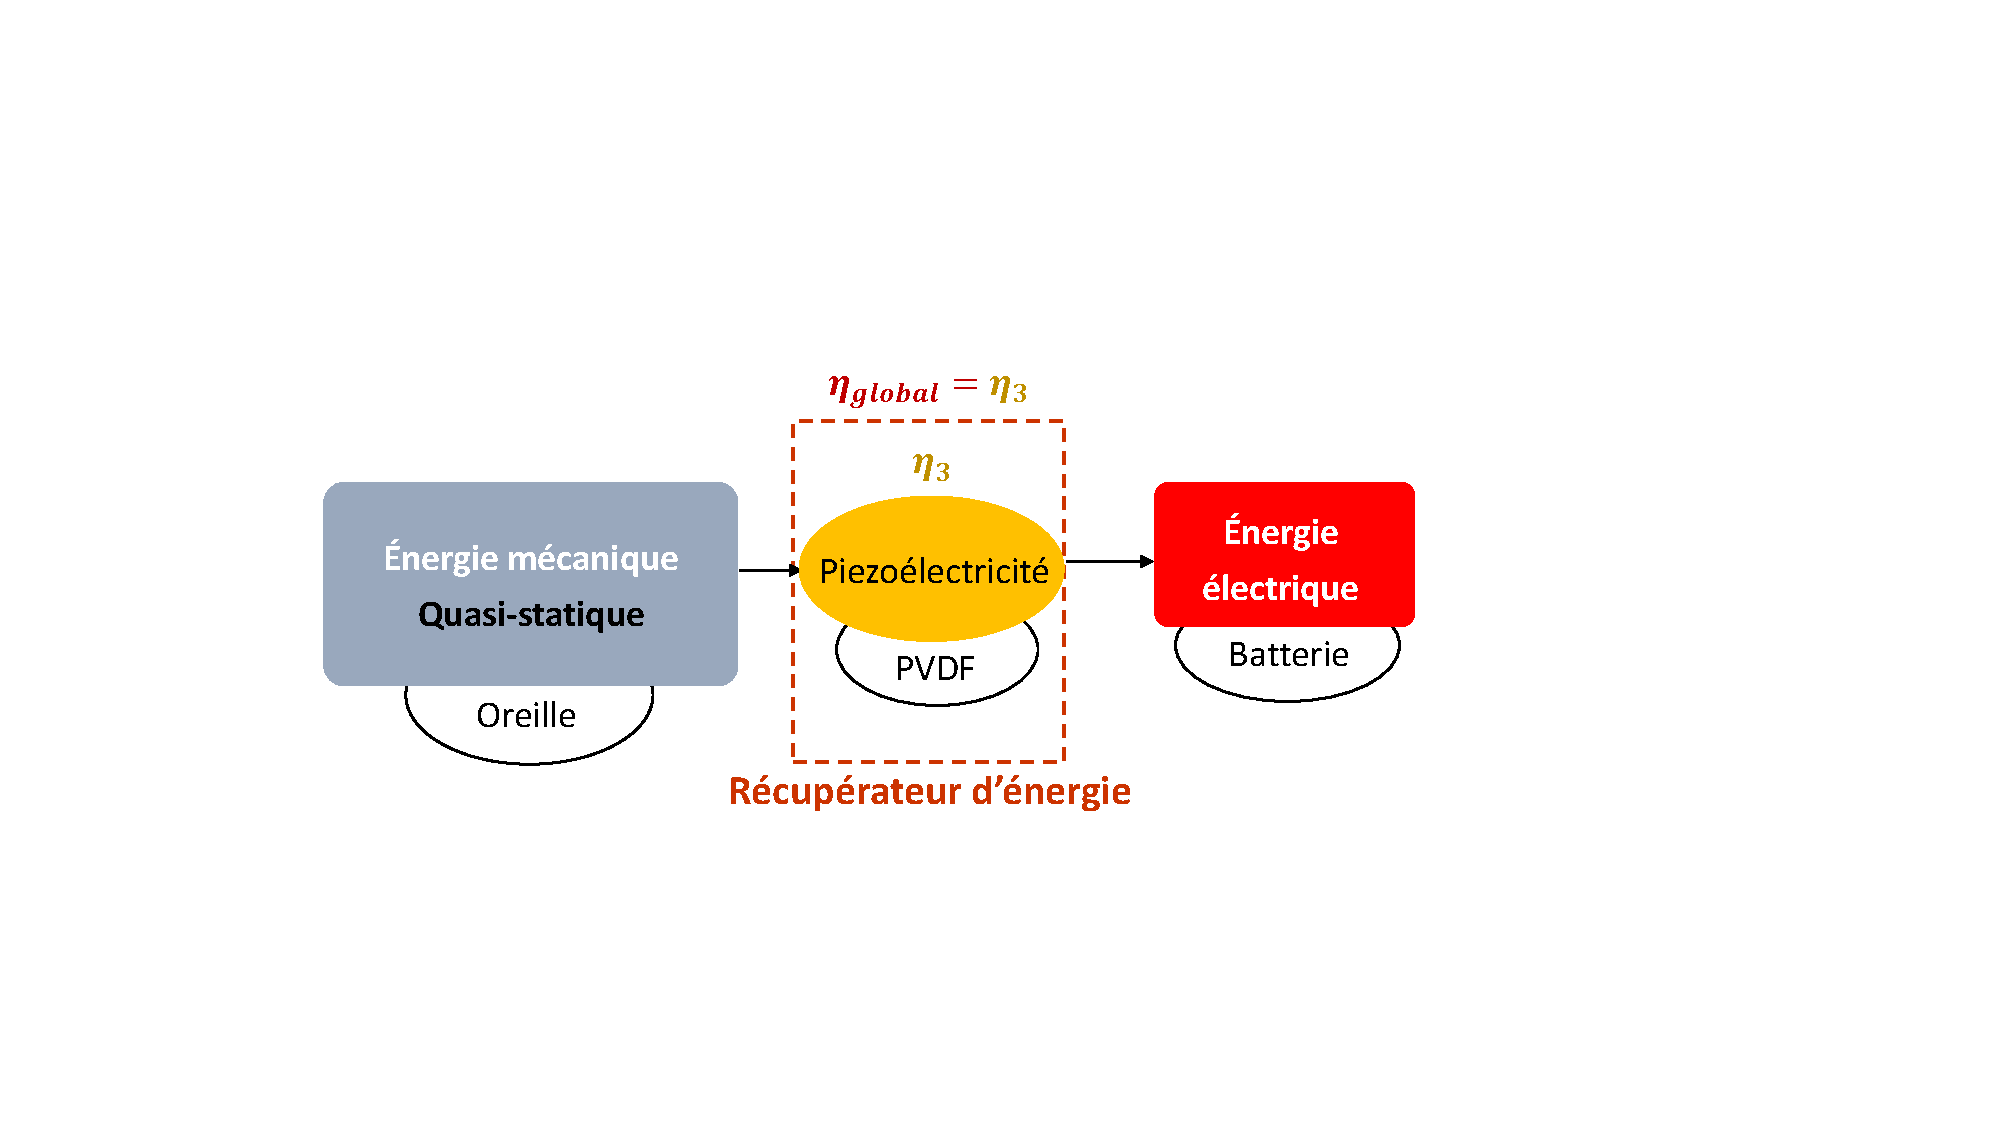
\includegraphics[trim={5cm 5cm 7cm 6cm},clip, width=0.7\textwidth]{../Chap2/Figure/conversion_critias_pvdf.pdf}
	\caption{Chaîne de conversion énergétique pour la solution piézoélectrique de \mbox{Delnavaz \& Voix \cite{Delnavaz2013}}}
	\label{fig:conversion_critias_pvdf}
\end{center}
\end{figure}
%%%%%%%%%%%%%%%%%%%%%%%%%%%%%%%%%%%%%%
\begin{figure}[!htbp]
\begin{center}
    \captionsetup{justification=centering}
	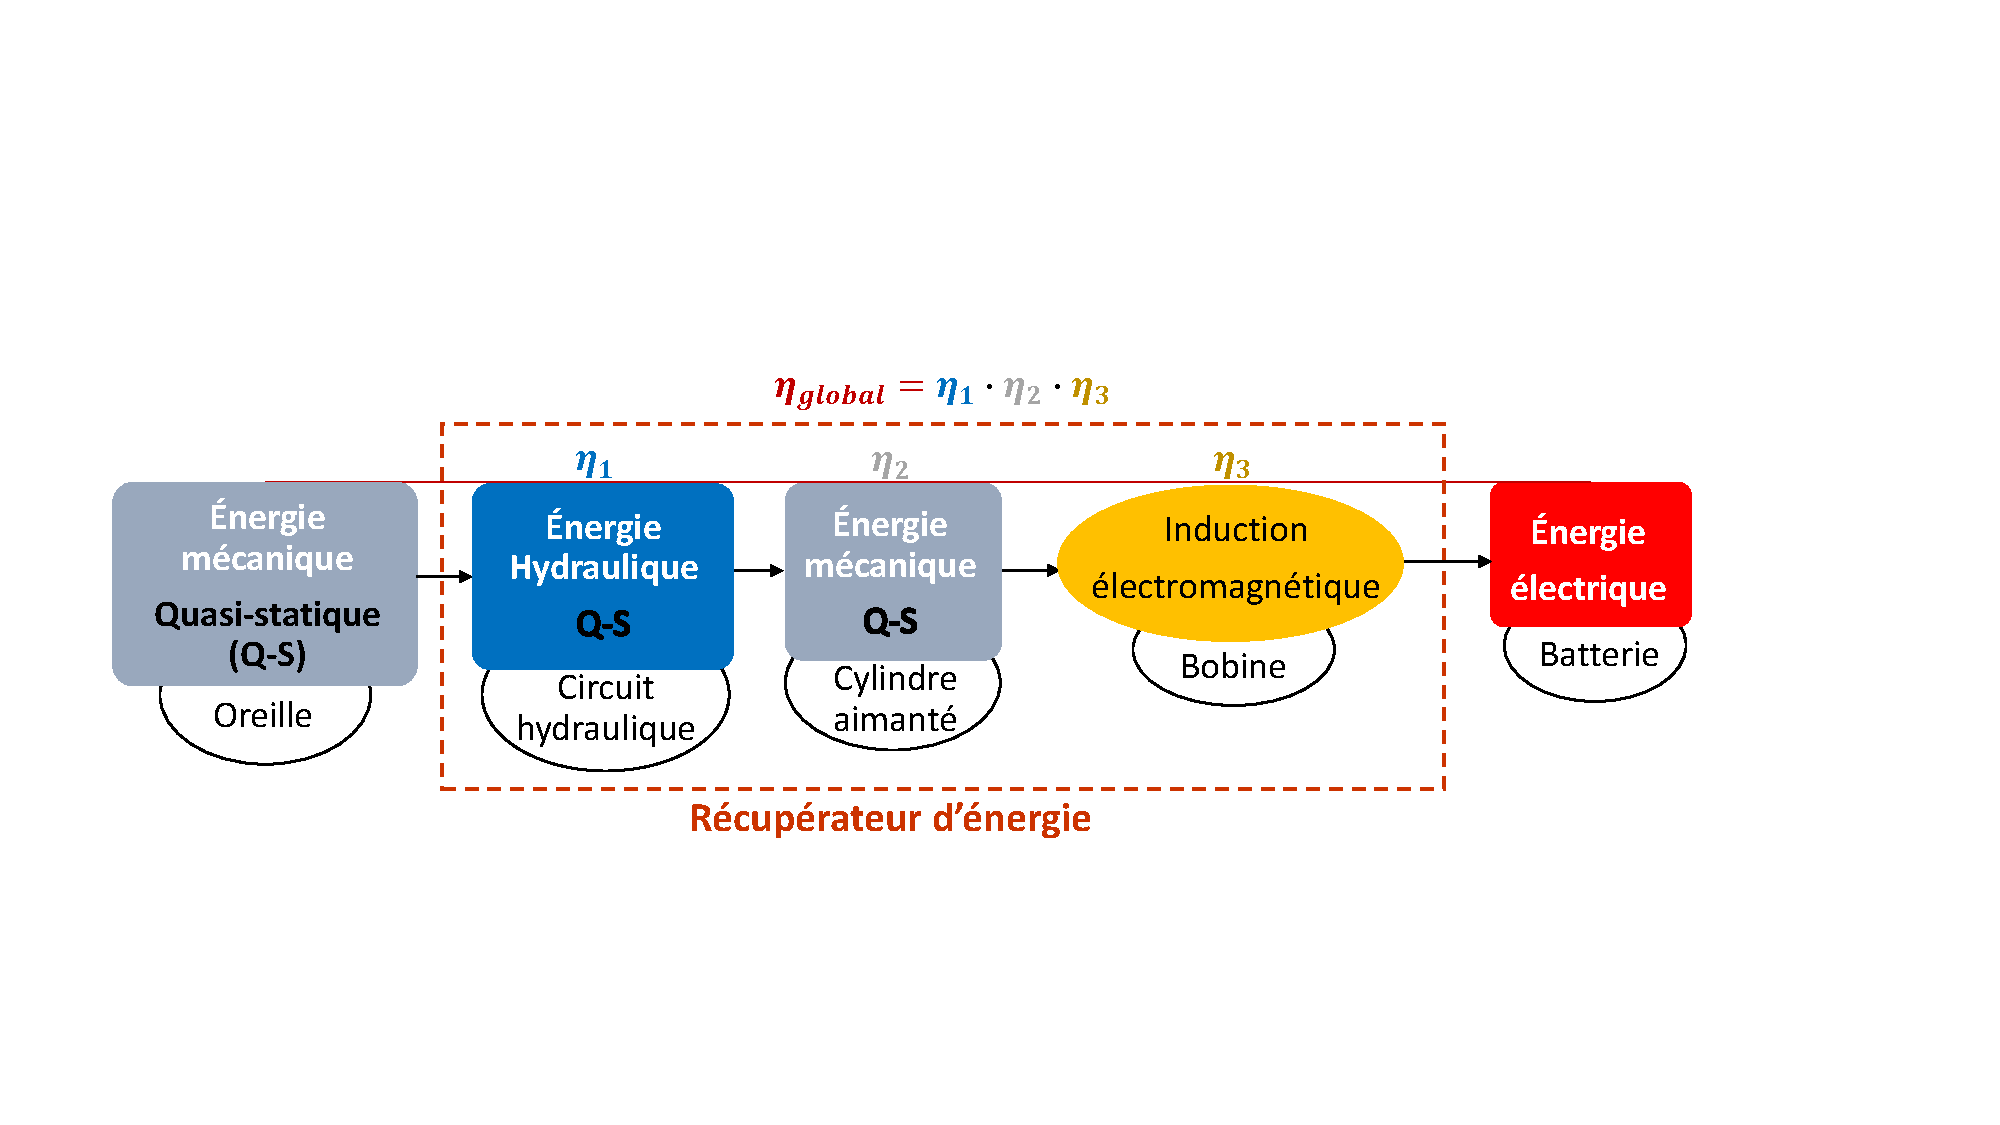
\includegraphics[trim={1cm 4.5cm 1cm 6cm},clip, width=\textwidth]{../Chap2/Figure/conversion_critias_electromag.pdf}
	\caption{Chaîne de conversion énergétique pour la solution électromagnétique de \mbox{Delnavaz \& Voix \cite{Delnavaz2014}}}
	\label{fig:conversion_critias_electromag}
\end{center}
\end{figure}
%%%%%%%%%%%%%%%%%%%%%%%%%%%%%%%%%%%%%%

Ce choix présente l'avantage de minimiser les étages de conversion, transformant ainsi la déformation mécanique du CA directement en énergie électrique au travers du phénomène de piézoélectricité. Le prototype ainsi fabriqué a été capable de récupérer 44µJ par cycle d'ouverture+fermeture de mâchoire. Il est cependant difficile d'établir un rendement de conversion pour le prototype, car l'énergie d'entrée n'a pas été quantifié. Néanmoins, nous avons vu que le coefficient de couplage électromécanique des polymères piézoélectriques est faible comparé à d'autres matériaux piézoélectriques plus rigides tels que les céramiques. Ces derniers présentent cependant le désavantage d'une impédance mécanique trop élevée pour être compatible avec un couplage direct efficace avec les tissus relativement mous du CA.

La seconde méthode, développée par la même équipe de chercheurs, consiste à exploiter un bouchon d'oreille rempli d'un fluide incompressible à l'instar d'une micro-pompe caractérisable par sa cylindrée $V_{ear}$ et sa pression $P_{ear}$. La cylindrée est définie comme le volume balayé dans le bouchon d'oreille pour un mouvement de mâchoire. La figure \ref{fig:Critias_electromag_schema} montre une vue schématisée de cette configuration de récupérateur. On établit la chaîne de conversion énergétique pour cette solution sur la figure \ref{fig:conversion_critias_electromag}.
%%%%%%%%%%%%%%%%%%%%%%%%%%%%%%%%%%%%%%
\begin{figure}[!htbp]
\begin{center}
    \captionsetup{justification=centering}
	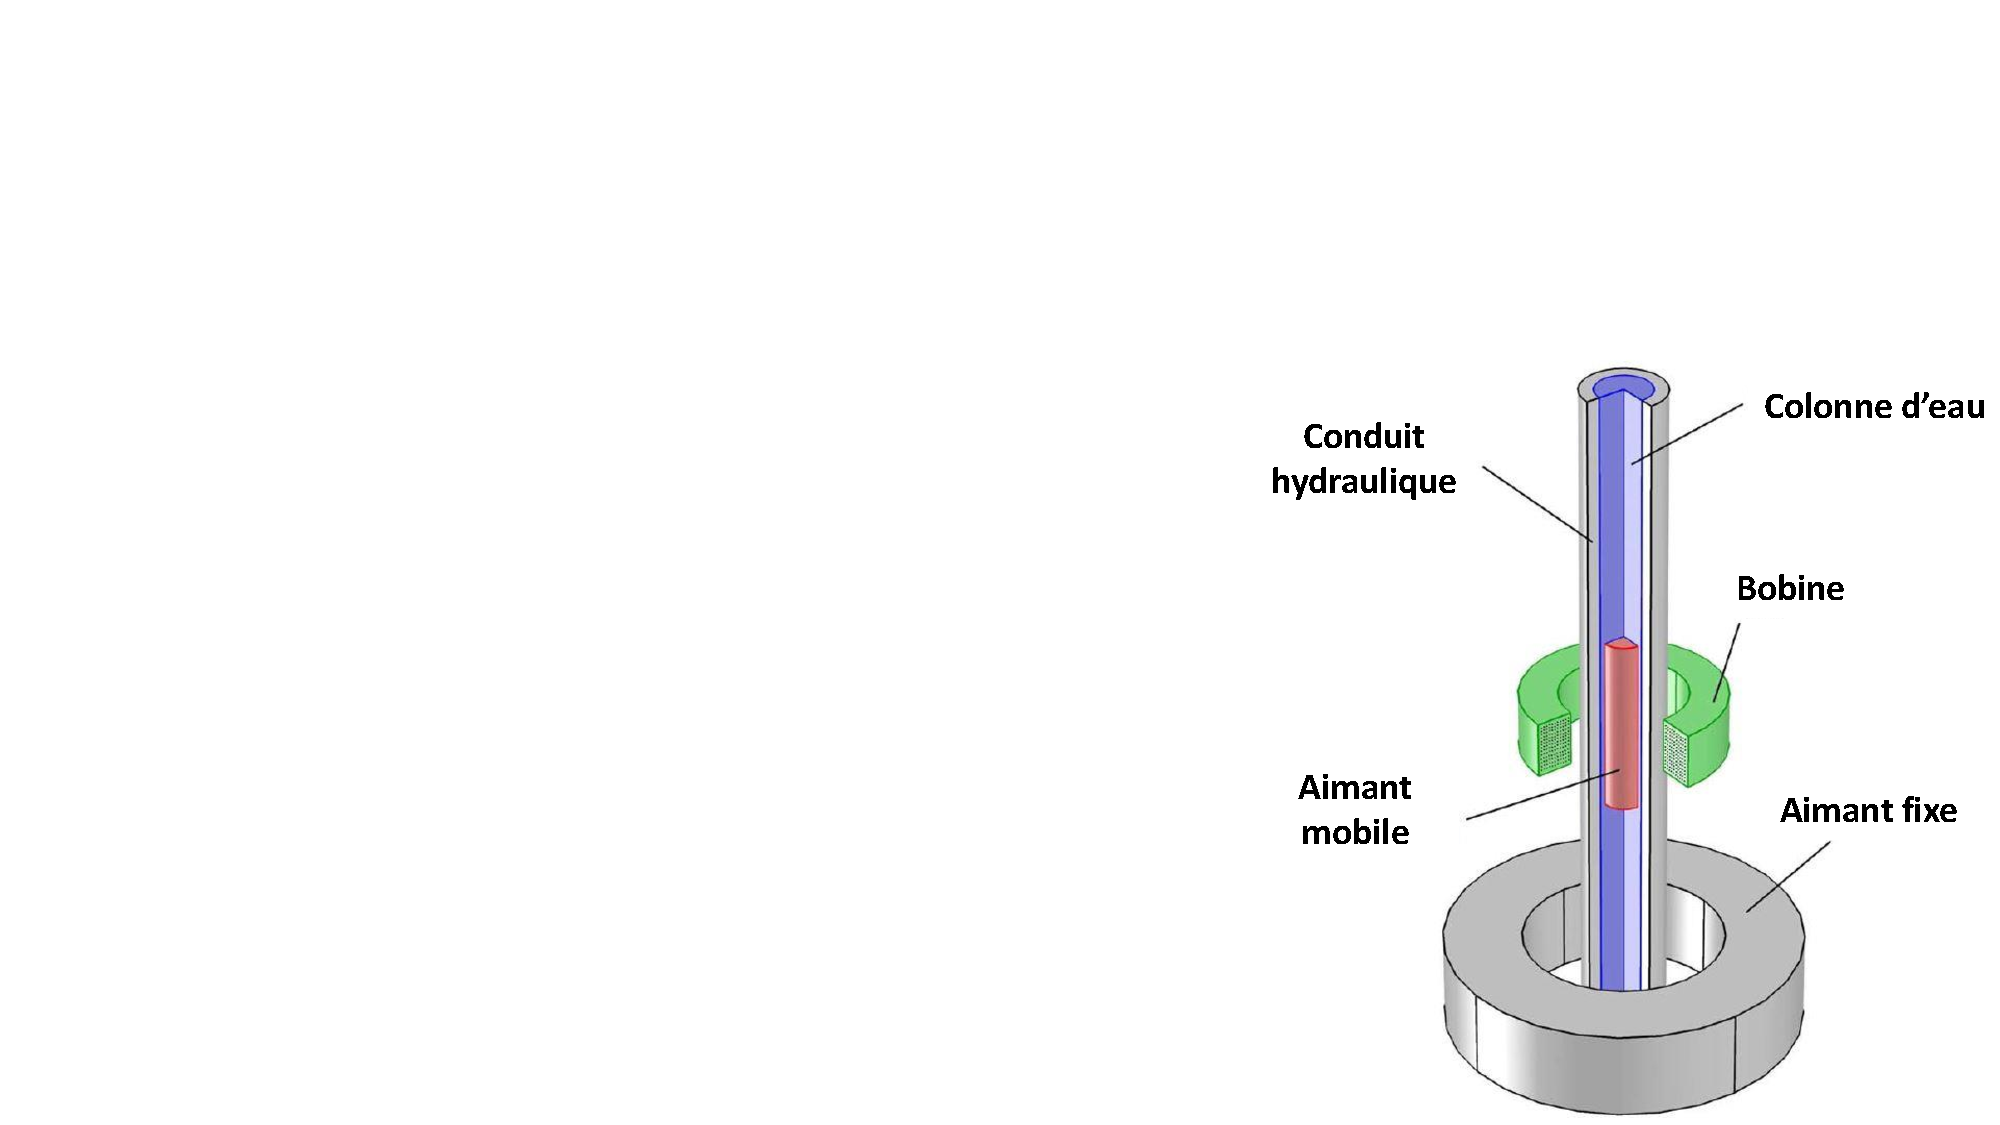
\includegraphics[trim={21cm 0cm 0cm 6cm},clip, width=0.3\textwidth]{../Chap2/Figure/Critias_electromag.pdf}
	\caption{Schéma du récupérateur d'énergie intra-auriculaire hydro-électromagnétique de \mbox{Delnavaz \& Voix \cite{Delnavaz2014}}}
	\label{fig:Critias_electromag_schema}
\end{center}
\end{figure}
%%%%%%%%%%%%%%%%%%%%%%%%%%%%%%%%%%%%%%

L'énergie de déformation mécanique du CA est d'abord transmise par la paroi interne de l'oreille au bouchon d'oreille. Ce transfert est possible par le maintien en position du bouchon contre le CA. À cet effet, le bouchon est moulé sur mesure et pressurisé après la pose afin d'épouser au mieux le CA. Le bouchon rempli de fluide transmet cette énergie au travers d'un circuit hydraulique à un cylindre magnétique qui agit comme un piston hydraulique. Une partie de cette énergie est ensuite dissipée par frottement lors du mouvement de l'aimant mobile et une autre partie est convertie par induction dans une bobine. Depuis la même source d'énergie que celle utilisée précédemment avec le récupérateur piézoélectrique, le prototype hydro-électromagnétique a été capable de récupérer 0.5$\micro$J par cycle d'ouverture + fermeture de mâchoire. Étant toujours difficile à quantifier, car dépendant de la source d'énergie en entrée du système, le rendement du convertisseur électromagnétique semble être nettement inférieur à celui du prototype piézoélectrique. Pour comprendre cela, nous pouvons nous appuyer sur la théorie de l'induction électromagnétique. En effet, la loi de Faraday montre que la puissance générée par induction électromagnétique est directement proportionnelle au carré de la vitesse de variation du flux magnétique qui la génère (éq. \ref{puissance_electromag}). Dans ce cas-ci, cette vitesse est celle de l'aimant mis en mouvement par le déplacement d'un volume de fluide, créant ainsi un champ magnétique variable dans la bobine.
\begin{equation}
	U_b = -N_b\biggl(\frac{d\Phi}{dt} \biggr)\\
	\label{faraday}
\end{equation}
	$U_b$ : Tension induite dans la bobine [$V$]\\
	$N_b$ : Nombre de tours de la bobine []\\
	$\Phi$ : Flux magnétique variable de l'aimant déplaceur [$Wb$]\\
	$t$ : Temps [$s$]\\
\begin{equation}
	P_{ch} = \frac{{U_b}^2}{R_{ch}}
	\label{puissance_UR}
\end{equation}	
	$R_{ch}$ : Résistance de charge [$\Omega$]\\
\begin{equation}
	P_{ch} = \biggl( \frac{{N_b}}{R_{ch}} \biggr)^2
			 \biggl( \frac{d\Phi}{dt} \biggr)^2
	\label{puissance_electromag}
\end{equation}	
	$P_{ch}$ : Puissance dissipée dans la résistance de charge [$W$]\\
\begin{figure}[!htbp]
\begin{center}
    \captionsetup{justification=centering}
	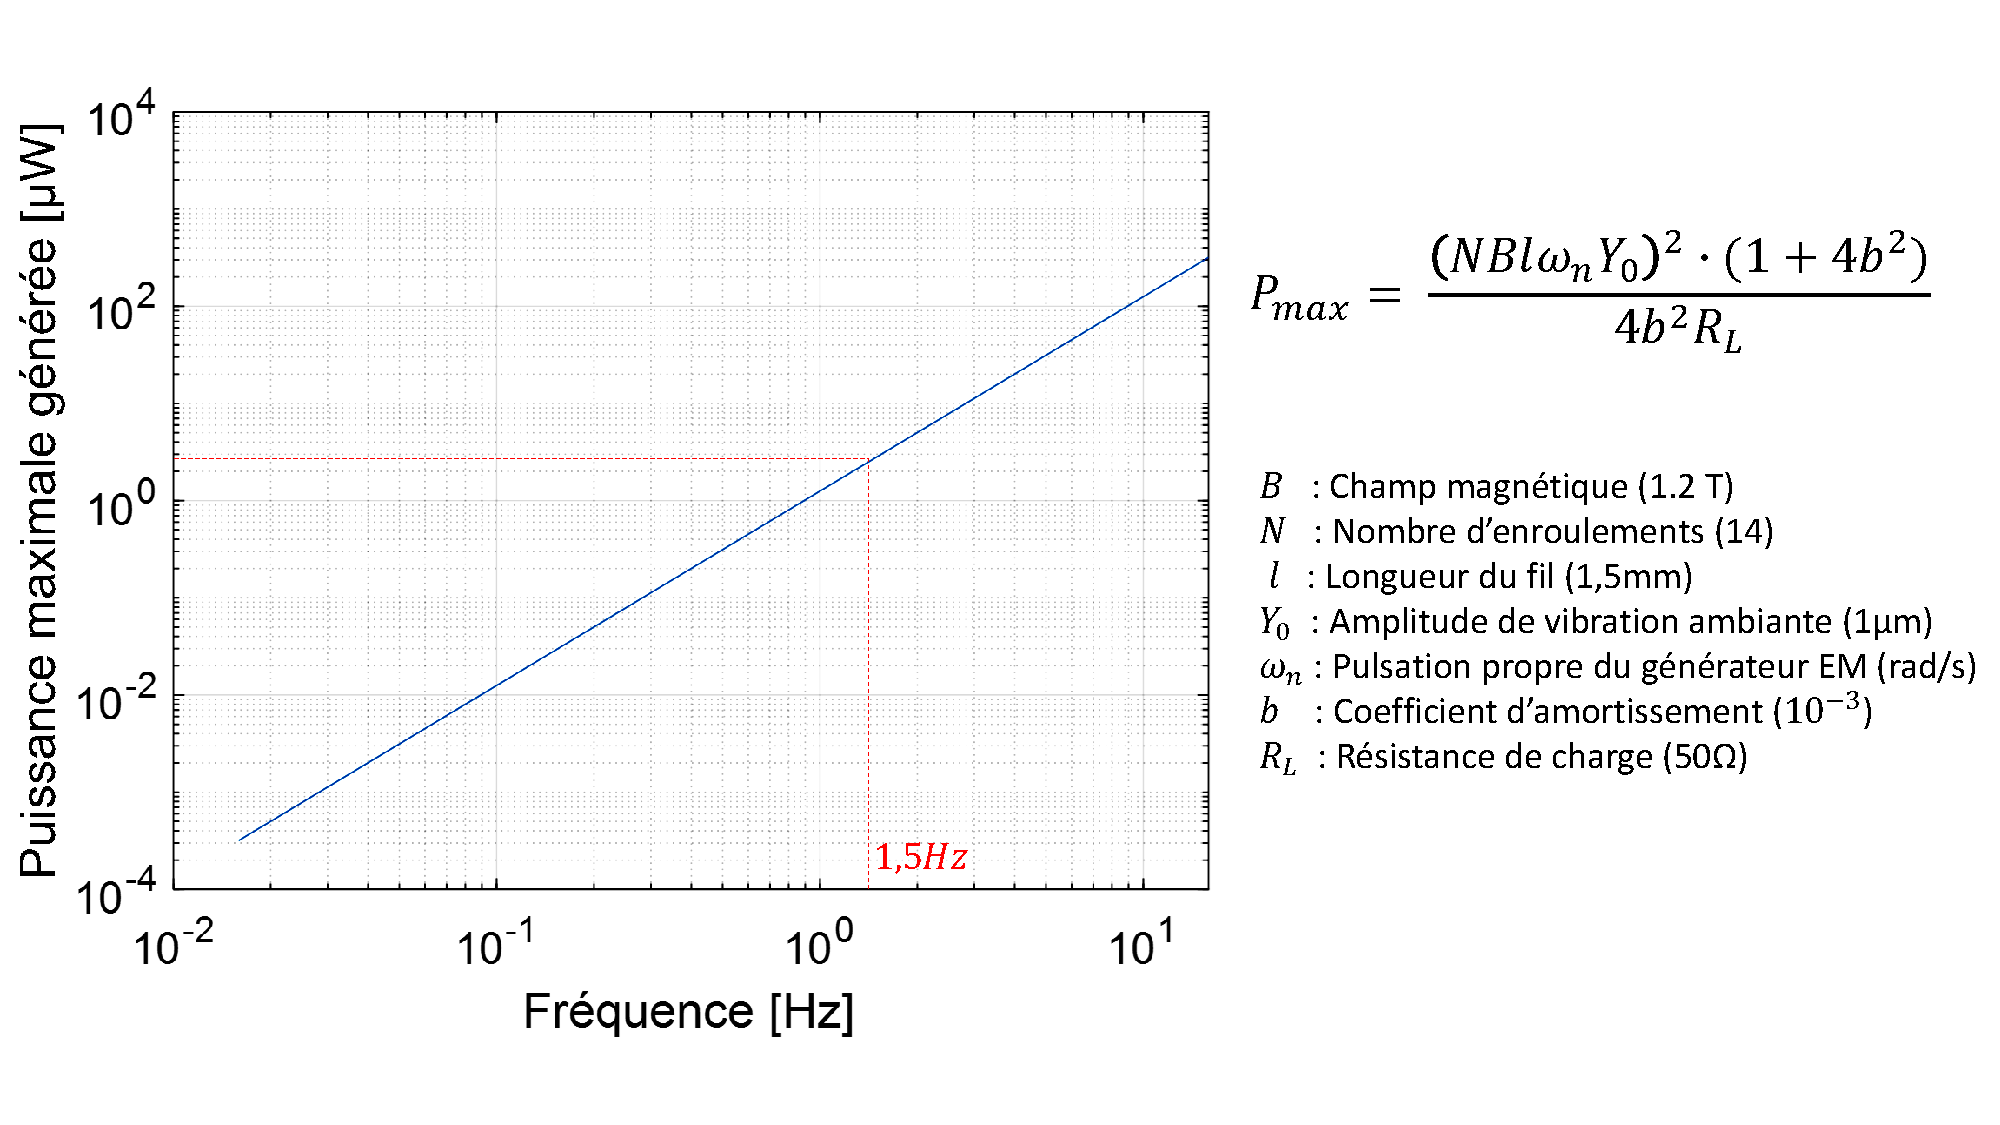
\includegraphics[trim={0cm 1cm 0cm 1cm},clip, width=0.8\textwidth]{../Chap2/Figure/puissance-frequence_electromag.pdf}
	\caption{Puissance électrique maximale d'un générateur EM pour différentes fréquences de fonctionnement \cite{Kulah2008}}
	\label{fig:puissance-frequence_electromag}
\end{center}
\end{figure}

La variation de flux magnétique est directement proportionnelle à la vitesse de déplacement de l'aimant permanent en mouvement, et donc à la fréquence de mastication de 1.57Hz. Cette-dernière est minimisée dans la configuration présente sur la figure \ref{fig:Critias_electromag_schema}. La figure \ref{fig:puissance-frequence_electromag} montre en effet la puissance maximale atteignable par un générateur électromagnétique (EM) en fonction de la fréquence de l'énergie d'excitation. Cette courbe suppose que la fréquence propre du générateur EM correspond à celle de l'excitation externe, et que la résistance interne de la bobine est négligeable devant la résistance de charge. Elle montre que la puissance maximale récupérable par un générateur EM est en théorie d'autant plus faible que sa fréquence d'excitation externe est basse. De plus, la fréquence propre du récupérateur hydro-électromagnétique de Delnavaz \emph{et al.} (fig. \ref{fig:Critias_electromag_schema}) n'a pas été adaptée à la fréquence de 1.57Hz de la mâchoire, ce qui minimise d'autant plus la puissance générée.

Par ailleurs, les dimensions d'un récupérateur d'énergie intra-auriculaire restent dans l'ordre de grandeur millimétrique. Cette contrainte amène plusieurs limitations qui peuvent baisser le rendement de conversion. Premièrement, cela limite la taille de la bobine induite intégrable et donc le nombre de spires, ainsi que la longueur de fil associée. Deuxièmement, on sait que la puissance récupérée est proportionnelle au carré de l'amplitude du déplacement de l'aimant mobile en regardant la figure \ref{fig:puissance-frequence_electromag}. En cherchant à augmenter celle-ci, il faut naturellement diminuer le diamètre du conduit hydraulique afin, que pour le même volume balayé, la course du cylindre soit plus importante. Cependant, les pertes de charges traduisant la dissipation d'énergie hydraulique (sec. \ref{sec:2.4_Modelisation du circuit hydraulique}) seront d'autant plus importantes que le diamètre du conduit sera faible. De plus, la densité de puissance d'un aimant permanent est directement proportionnelle au carré de son volume qui ici s'en retrouvera aussi diminué \cite{Priya2017}. Cette stratégie de récupération permet néanmoins de transférer l'énergie à l'extérieur du CA afin de tirer profit de méthodes de transduction différentes qui auraient été plus complexes, voire impossibles à intégrer dans l'oreille par souci d'encombrement.

Des travaux comme ceux de Priya \emph{et al.} ont visé à estimer l'impact de la réduction d'échelle pour les dispositifs de récupération d'énergie \cite{Marin2011}. En effet, il en résulte que la puissance produite est directement proportionnelle au volume effectif $V_m$ du matériau de conversion électromécanique. En prenant en considération les équations respectives de chacune des méthodes de transduction, la puissance électromagnétique générée est proportionnelle à ${V_m}^2$; tandis que la puissance piézoélectrique est elle proportionnelle à ${V_m}^{\frac{3}{4}}$. Cela implique, qu'avec la réduction d'échelle, la transduction piézoélectrique devient plus efficace que l'électromagnétique. En regardant alors la figure \ref{fig:puissance-volume} établie dans les travaux de Marin \cite{Marin2011}, on peut tracer une droite de régression linéaire pour estimer la tendance de l'évolution de la puissance produite en fonction du volume effectif du dispositif.
%%%%%%%%%%%%%%%%%%%%%%%
\begin{figure}[!htbp]
\begin{center}
    \captionsetup{justification=centering}
	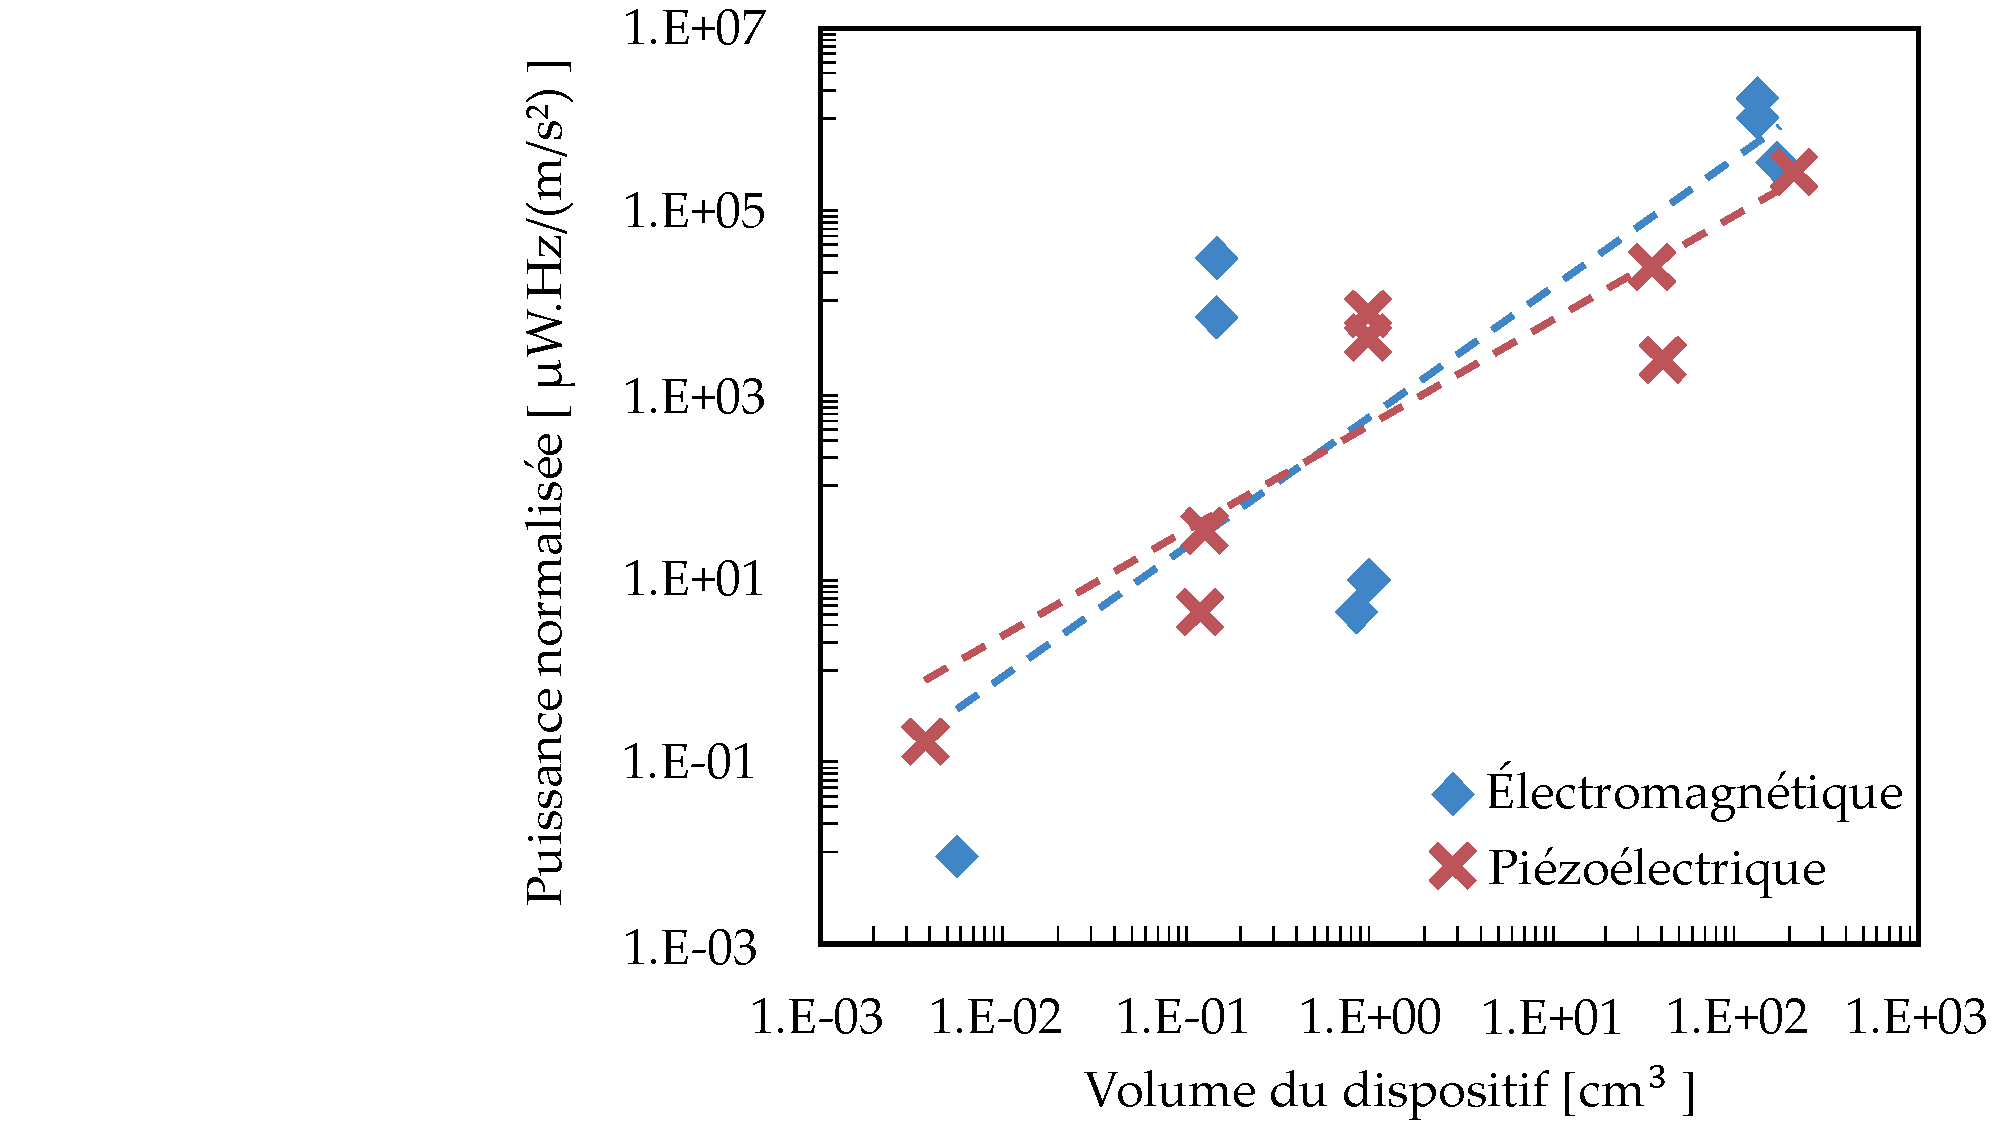
\includegraphics[trim={8cm 0cm 0cm 0cm},clip,width=0.7\textwidth]{../Chap2/Figure/puissance-volume.pdf}
	\caption{Puissance générée en fonction du volume effectif du matériau pour les mécanismes de récupération d'énergie par vibration piézoélectrique et électromagnétique. Puissance de sortie normalisée par l'accélération et multipliée par la fréquence en fonction du volume effectif du matériau de transduction considéré pour divers récupérateurs d'énergie trouvés dans la littérature et dans le commerce. \cite{Priya2017}}
	\label{fig:puissance-volume}
\end{center}
\end{figure}
%%%%%%%%%%%%%%%%%%%%%%%

On relève alors qu'à partir d'un volume critique d'environ $0.5$cm$^3$ la conversion piézoélectrique devient plus efficace que la conversion électromagnétique pour le même volume effectif de matériau respectif. Les dispositifs de récupération d'énergie développés en vue d'exploiter l'énergie de déformation du CA sont d'après la littérature en deçà de cette limite (tab. \ref{tab:volume_protos_critias}). Il sera donc pertinent de privilégier la piézoélectricité pour notre application.\\
%%%%%%%%%%%%%%%%%
\begin{table}[!htbp]
	\centering
	\captionsetup{justification=centering}
	\rowcolors[]{2}{black!8}{}{
		\begin{tabular}{ m{0.3\textwidth} c c }
			\rowcolor{blue!10}
			\toprule
			\textbf{Dispositif}                         & \textbf{Volume [cm$^3$]} & \textbf{Puissance moyenne [$\micro$W]} \\
			\midrule
			Anneau piézoélectrique  \cite{Delnavaz2013} & $5\cdot10^{-2}$                     & 70                                     \\
			Patch piézoélectrique   \cite{Carioli2018}  & $5.5\cdot10^{-3}$                    & 0.2                                    \\
			Hydro-électromagnétique	\cite{Delnavaz2014} & $6.5\cdot10^{-3}$                    & 0.3                                    \\
			\bottomrule
		\end{tabular}}
	\caption{Volume de matériau effectif pour les dispositifs développés pour l'exploitation de l'énergie dissipée par la mastication d'après la littérature}
	\label{tab:volume_protos_critias}
\end{table}
%%%%%%%%%%%%%%%%%%%%%      
%%%%%%%%%%%%%%%%%%%%%%%
\begin{figure}[!htbp]
\begin{center}
    \captionsetup{justification=centering}
	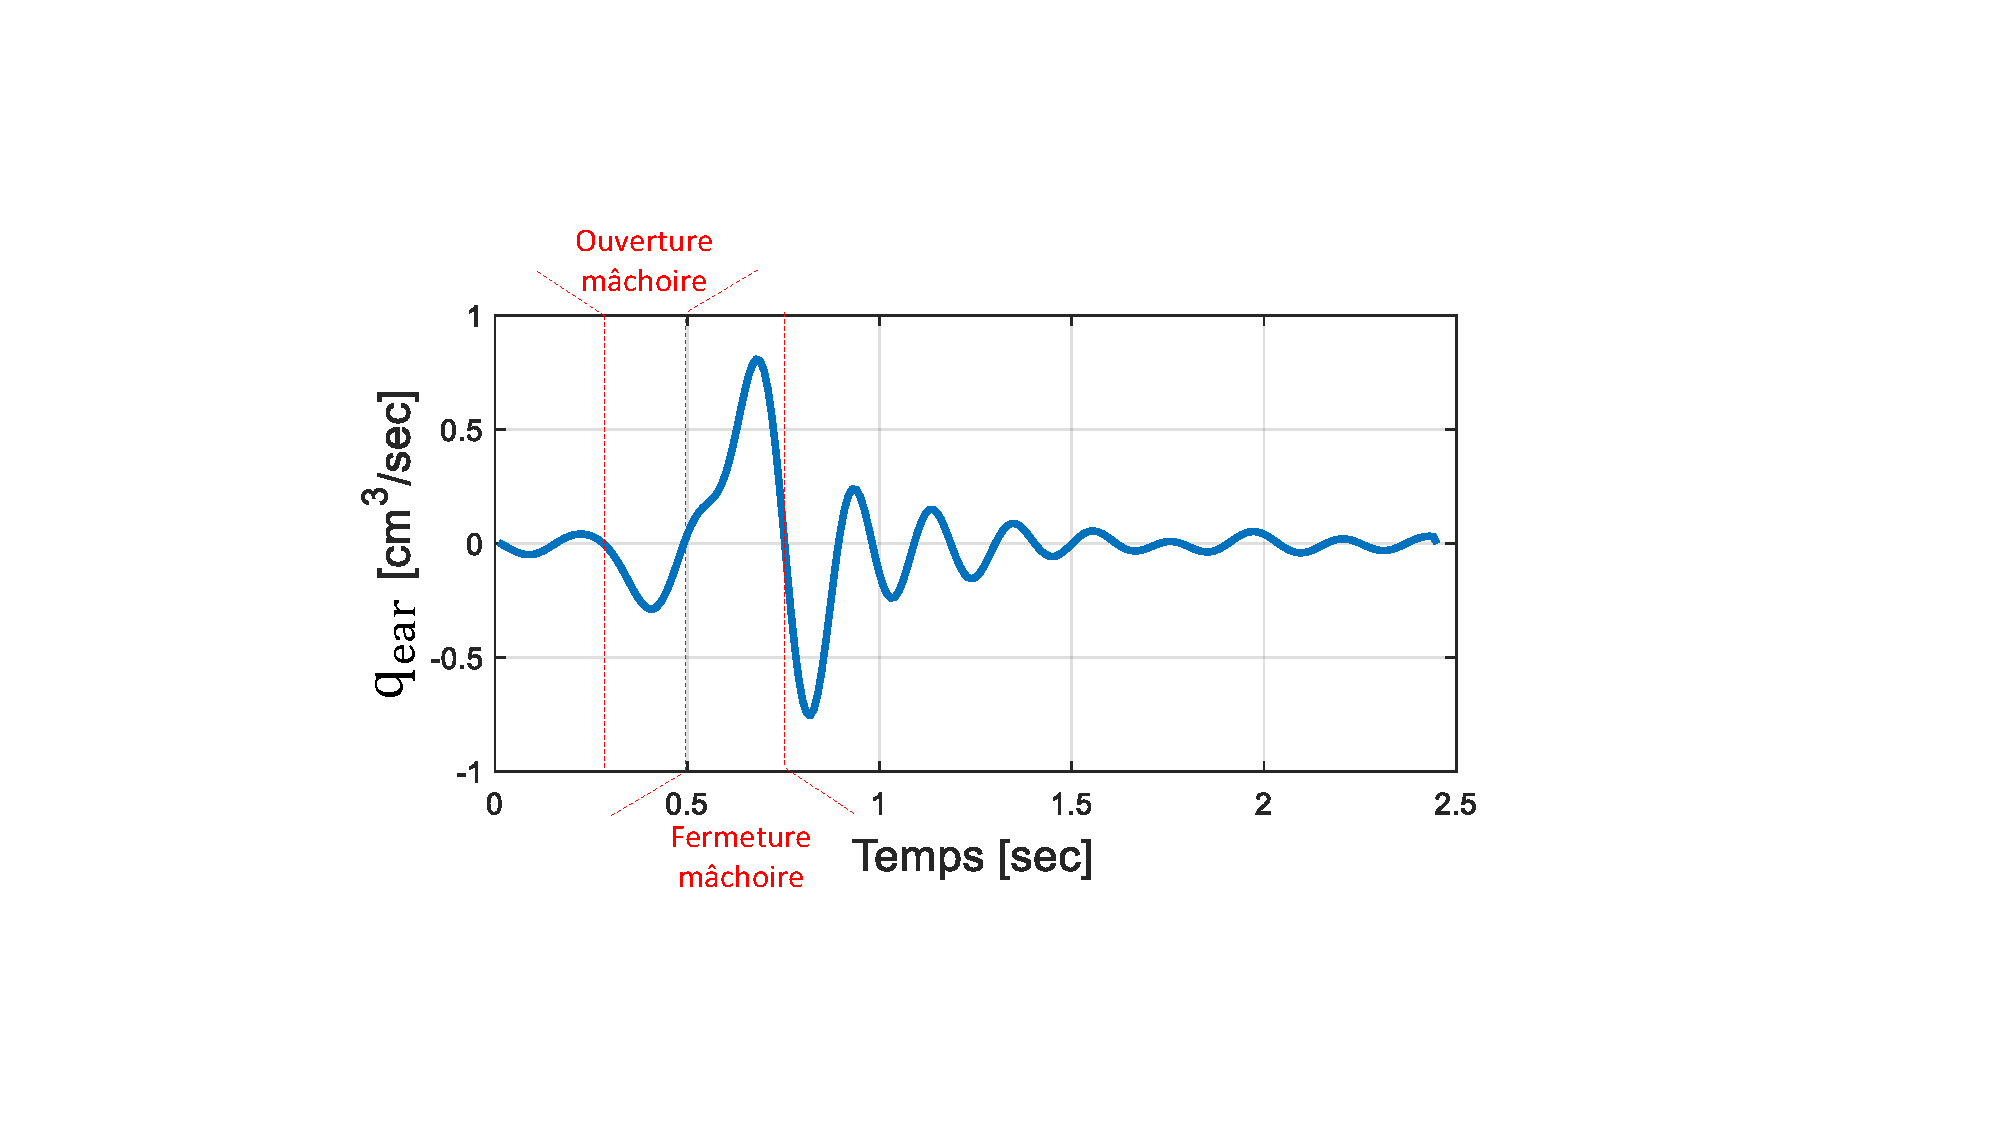
\includegraphics[trim={6cm 3.5cm 8.5cm 3.5cm},clip,width=0.5\textwidth]{../Chap2/Figure/debit.pdf}
	\caption{Débit de fluide depuis le bouchon d'oreille sur 1 cycle de mastication \cite{Delnavaz2012}}
	\label{fig:debit_ear}
\end{center}
\end{figure}
%%%%%%%%%%%%%%%%%%%%%%%

On sait par ailleurs que l'étage hydraulique amène des pertes supplémentaires par rapport à une solution de type bouchon d'oreille PVDF. Ces pertes peuvent être de deux natures : les pertes mécaniques par frottement et les pertes de charges hydrauliques. Le premier type de pertes découle de la conversion hydromécanique qui nécessite d'avoir une pièce en mouvement, généralement un piston hydraulique, poussée par la pression du fluide. Le joint d'étanchéité qui y est intégré induit des pertes par frottement mécanique entre le piston et la chambre du piston. Le second type de pertes est lié à la baisse de pression se produisant le long d'un écoulement dans une conduite. Celle-ci résulte du frottement du fluide contre la paroi du conduit et peut aussi être la cause de singularités géométriques tels qu'un coude ou un changement de section dans ce même conduit. Ces pertes hydrauliques sont directement proportionnelles au débit de l'écoulement et dépendent du nombre de Reynolds $Re$ défini à l'équation \ref{eq:Reynolds}.
\begin{equation}
	Re = \dfrac{4\ \rho\ q_{ear}}{\pi\ \mu\ D}
\label{eq:Reynolds}
\end{equation}
$\rho$ : Masse volumique du fluide [kg/m$^3$]\\
$D$ :   Diamètre du conduit [m] \\
$\mu$ :  Viscosité dynamique du fluide [Pa.s] \\
$q_{ear}$ : Débit sortant du bouchon d'oreille [m$^3$/s]\\

Elles sont d'autant plus importantes que le nombre de Reynolds augmente \cite{Fady1988}. En nous basant sur les données expérimentales de Delnavaz \emph{et al.}, on peut tracer l'évolution du débit sortant du bouchon d'oreille, précédemment introduit pour la solution hydro-électromagnétique, sur la figure \ref{fig:debit_ear}. Avec les dimensions du dispositif illustré sur la figure \ref{fig:Critias_electromag_schema}, Re=510. On considère que l'écoulement est laminaire (Re<2000) et que les pertes de charges sont par conséquent faibles. Pour le même débit maximal, l'écoulement serait turbulent (Re>2000) si $D<0.5mm$. Le détail de la modélisation de ces pertes énergétiques sera détaillé dans la suite lors de la modélisation du circuit hydraulique. Ce que nous retenons avec l'estimation de Re est que les pertes hydrauliques en écoulement laminaire seront modérées si on reste dans l'ordre de grandeur millimétrique pour le diamètre du circuit. Par ailleurs, les pertes de charges singulières font aussi partie des dissipations hydrauliques. Clles-ci sont générées par les irrégularités dans la géométrie du circuit hydraulique et sont probablement prépondérantes pour une telle application. Elles doivent donc être quantifiées pour être minimisés devant l'énergie disponible.
    %/////////////////////////////////////////////
	\subsection{Conclusion sur la récupération d'énergie dans le CA}
	\label{subsec:1.4.4_onclusion sur la recuperation d energie dans le CA}
	%////////////////////////////////////////////
La littérature nous guide dans les choix technologiques pouvant aider à maximiser l'énergie exploitable depuis la déformation mécanique du CA.\\
Voici les éléments sur lesquels nous nous appuyons pour établir une proposition de récupérateur optimale d'après les informations disponibles dans la littérature à ce jour :
\begin{enumerate}
\item %$$$$$$$$$$$$$
Il est intéressant d'exploiter une source d'énergie hydraulique quasi-statique (QS) pour deux raisons majeures : 
\begin{itemize}[label=$\circ$]
	\item \emph{Limiter les pertes énergétiques par transport} grâce aux débits faibles en jeu dans le bouchon d'oreille (figure \ref{fig:debit_ear})
		\item \emph{Tirer profit d'un volume de travail disponible plus important} en transférant la source d'énergie hors du CA.
\end{itemize}	
\item %$$$$$$$$$$$$$
La transduction piézoélectrique est à privilégier pour des sources d'énergie basse fréquence (<10Hz) avec des contraintes d'encombrement imposant des dispositifs à faibles volumes. De plus, l'implémentation de structures en céramiques piézoélectriques maximiserait le coefficient de couplage électromécaniques du système.
\item %$$$$$$$$$$$$$
La conversion \emph{frequency-up} au moyen de structures mécaniques oscillantes est un moyen efficace pour amplifier la fréquence de la source d'énergie et ainsi augmenter les puissances de sortie des récupérateurs.
\end{enumerate}	  
%/!\/!\/!\/!\/!\/!\/!\/!\/!\/!\/!\/!\/!\/!\/!\/!\/!\/!\/!\/!\/!\/!\/!\/!\%
\section{Présentation des travaux de thèse}
\label{sec:1.5}
%/!\/!\/!\/!\/!\/!\/!\/!\/!\/!\/!\/!\/!\/!\/!\/!\/!\/!\/!\/!\/!\/!\/!\/!\%
Cette thèse propose une architecture innovante qui répond aux besoins primordiaux d'un système de valorisation de l'énergie de déformation mécanique du CA, à savoir : respecter le confort de l'utilisateur, s'adapter au volume restreint du CA, maximiser la transmission d'efforts depuis les tissus mous du corps humain et s'adapter à la faible fréquence de la source.

Le chapitre \ref{ch:2_Modelisation et simulation du systeme} présente l'architecture de récupérateur, spécialement conçue et dimensionnée pour l'application. Celle-ci tend à maximiser le rendement de conversion à l'aide des solutions proposées dans la littérature. Une modélisation multiphysique du système hydro-piézoélectrique amplifié est alors proposée et un nouveau concept de valve hydraulique y est introduit.
Le chapitre \ref{ch:3_Conception et fabrication du convertisseur electromecanique : OB + GPA} se concentre ensuite autour de la caractérisation expérimentale du convertisseur électromécanique HF composé d'un oscillateur bistable et d'un flextenseur associé à un empilement de céramiques piézoélectriques. Le chapitre \ref{ch:4_Valves hydrauliques a base de tubes flexibles flambes} présente la caractérisation expérimentale des valves hydrauliques introduites précédemment, puis le chapitre \ref{ch:5_Approche theorique pour la modelisation des VH} proposant une modélisation du comportement théorique de ces derniers. Enfin, le chapitre \ref{ch:6_Comportement du systeme de recuperation d’energie intra-auriculaire avec les composants caracterises experimentalement} montre la corrélation modèle-essais générale avec les éléments caractérisés expérimentalement. L'influence des différents paramètres sur les performances du système sont discutés et des pistes d'améliorations sont proposées.









% Le corps humain génère en effet une multitude de signaux biophysiques (température, biopotentiel, motricité) et biochimiques (électrolytes, métabolites) qui définissent son état de fonctionnement. Des dispositifs actifs et passifs permettent alors de mesurer, et dans certains cas, de réguler ces derniers afin de les garder dans leurs intervalles de tolérances respectifs.


%Ce dernier se base sur l'arrachement d'électrons au sein de la matrice du matériau semi-conducteur par l'énergie apportée par un photon. Une différence de potentiel se crée alors entre les deux faces, permettant ainsi la génération de tension comme dans une pile à combustible.

% De conception similaire aux piles à combustible, ces réacteurs génèrent de l’électricité à partir des réactions d’oxydo-réduction impliquées dans la dégradation de molécules organiques par les bactéries, aboutissant à la libération de protons et d’électrons qui peuvent être transférés aux électrodes.

% %%%%%%%%%%%%%%%%%%%%%%%%%%%%%%%%%%%%%%
% \begin{table}[!htbp]
% 	\centering
% 	\resizebox{\textwidth}{!}{%
% 	\begin{tabular}{ c c c c }
% 	\toprule
% 	\multicolumn{2}{c}{\textbf{Source d'énergie}} 	& 	& 	\\
% 	\cmidrule[0.3pt]{1-2}
% 	\multicolumn{1}{c}{\textbf{Nature}} & \multicolumn{1}{c}{\textbf{Source}}
% 	&	\multicolumn{1}{c}{\multirow{-2}{*}{\textbf{Méthode de transduction}}}								
% 	&	\multicolumn{1}{c}{\multirow{-2}{*}{\textbf{Références}}}	\\ 						 	
% 	\cmidrule[2pt]{1-4}
% 	%%%%%%%%%%
% 	&&	Thermoélectricité				&	\\	\cmidrule[0.3pt]{3-4}
% 	\multirow{-2}{*}{Thermique}			&	\multirow{-2}{*}{Chaleur corporelle}	
% 	&	Pyroélectricité					&	\\	\hline
% 	%%%%%%%%%%
% 	&&	Photovoltaïque					& \cite{Zhao2020}	\\	\cmidrule[0.3pt]{3-4}
% 	\multirow{-2}{*}{Lumière}			&	\multirow{-2}{*}{Soleil}
% 	&	Photoélectricité				&	\\	\hline		
% 	%%%%%%%%%%
% 	Radiofréquence						&	Rayonnement cellulaire	
% 	& Antenne redresseuse				&	\\	\hline		
% 	%%%%%%%%%%	
% 	Chimique							&	Chimie cellulaire	
% 	& Piles à combustible microbiennes	&	\\	\hline
% 	%%%%%%%%%%
% 	&&	Induction électromagnétique		&	\\	\cline{3-4}
% 	&&	Piézoélectricité				&	\\	\cmidrule[0.3pt]{3-4}
% 	&&	Électro statisme				&	\\	\cmidrule[0.3pt]{3-4}
% 	\multirow{-4}{*}{Mécanique}			&	\multirow{-4}{*}{Mouvement ou déformation}	
% 	&	Triboélectricité				&	\\	
% 	%%%%%%%%%%
% 	\bottomrule
% 	\end{tabular}}
% 	\caption{Technologies de récupération d'énergie sur le corps humain}
% 	\label{tab:Technologies de recuperation d'energie sur le corps humain}
% 	\end{table} 
% 	%%%%%%%%%%%%%%%%%%%%%%%%%%%%%%%%%%%%%%%